\documentclass[11pt]{scrreprt}
\usepackage[sexy]{evan}
\renewcommand{\figurename}{Image}
\numberwithin{figure}{chapter}

\begin{document}
\title{The 55th International Mathematical Olympiad}
\subtitle{Cape Town, South Africa}
\author{Evan Chen}
\date{July 2014}
\maketitle

\tableofcontents

\chapter{Problems}
It appears that the protocol for 1, 2, 4, 5 being distinct subjects is still in effect.
Unfortunately, this has forced the inclusion of Problem 5 as a fake N which is really C, making this an
IMO with three combinatorics problems.
\section{Day 1}
\begin{problem}
  Let $a_0 < a_1 < a_2 \ldots$ be an infinite sequence of positive integers. Prove that there exists a unique integer $n\geq 1$ such that \[a_n < \frac{a_0+a_1+a_2+\cdots+a_n}{n} \leq a_{n+1}.\]
\end{problem}
\begin{problem}
  Let $n \ge 2$ be an integer. Consider an $n \times n$ chessboard consisting of $n^2$ unit squares. A configuration of $n$ rooks on this board is \emph{peaceful} if every row and every column contains exactly one rook. Find the greatest positive integer $k$ such that, for each peaceful configuration of $n$ rooks, there is a $k \times k$ square which does not contain a rook on any of its $k^2$ unit squares.
\end{problem}
\begin{problem}
  Convex quadrilateral $ABCD$ has $\angle ABC = \angle CDA = 90^{\circ}$. Point $H$ is the foot of the perpendicular from $A$ to $BD$. Points $S$ and $T$ lie on sides $AB$ and $AD$, respectively, such that $H$ lies inside triangle $SCT$ and \[
\angle CHS - \angle CSB = 90^{\circ}, \quad \angle THC - \angle DTC = 90^{\circ}. \] Prove that line $BD$ is tangent to the circumcircle of triangle $TSH$.
\end{problem}

\section{Day 2}
\begin{problem}
  Let $P$ and $Q$ be on segment $BC$ of an acute triangle $ABC$ such that $\angle PAB=\angle BCA$ and $\angle CAQ=\angle ABC$. Let $M$ and $N$ be the points on $AP$ and $AQ$, respectively, such that $P$ is the midpoint of $AM$ and $Q$ is the midpoint of $AN$. Prove that the intersection of $BM$ and $CN$ is on the circumference of triangle $ABC$.
\end{problem}
\begin{problem}
  For every positive integer $n$, the Bank of Cape Town issues coins of denomination $\frac 1n$.
  Given a finite collection of such coins (of not necessarily different denominations) with total value at most $99 + \half$, prove that it is possible to split this collection into $100$ or fewer groups, such that each group has total value at most $1$.
\end{problem}
\begin{problem}
  A set of lines in the plane is in \emph{general position} if no two are parallel and no three pass through the same point. A set of lines in general position cuts the plane into regions, some of which have finite area; we call these its \emph{finite regions}.
  Prove that for all sufficiently large $n$, in any set of $n$ lines in general position it is possible to colour at least $\sqrt{n}$ lines blue in such a way that none of its finite regions has a completely blue boundary.

  \emph{Note:} Results with $\sqrt{n}$ replaced by $c\sqrt{n}$ will be awarded points depending on the value of the constant $c$.
\end{problem}


\chapter{Results}
Taiwan ranks $3$rd with a total of $192$ and awards GGBBGG.
One point ahead is the United States, and with $203$ points is China.
This is one of the strongest results Taiwan has obtained.

The cutoffs were 16 for Bronze, 22 for Silver, 29 for Gold.

Presented below are the full names and results of the Taiwan IMO team.

\begin{table}[ht]
  \centering
  \begin{tabular}[h]{|l|l|c|rrrrrr|cl|}
    \hline \multicolumn{2}{|l|}%
    {Name}                 & Code &P1 &P2 &P3 &P4 &P5 &P6 & $\Sigma$ & Awards \\ \hline
    Chao Ting-Wei & 趙庭偉 & TWN1 & 7 & 6 & 7 & 7 & 6 & 5 & 38 & Gold, 7th  \\ \hline
    Chen Evan     & 陳誼廷 & TWN2 & 7 & 7 & 7 & 7 & 7 & 1 & 36 & Gold, 12th  \\ \hline
    Chen Po-Rui   & 陳柏叡 & TWN3 & 7 & 5 & 0 & 7 & 2 & 0 & 21 & Bronze, 163rd \\ \hline
    Wu Pang-Cheng & 吳邦誠 & TWN4 & 7 & 6 & 0 & 7 & 0 & 0 & 20 & Bronze, 200th  \\ \hline
    Wu Po-Sheng   & 吳博生 & TWN5 & 7 & 7 & 7 & 7 & 7 & 7 & 42 & Gold, 1st \\ \hline
    Yu Hung-Hsun  & 余竑勳 & TWN6 & 7 & 7 & 7 & 7 & 7 & 0 & 35 & Gold, 15th \\ \hline
  \end{tabular}
  \caption{IMO Results for Taiwan 2014.}
\end{table}


Roger Lin is team leader and Sen-Peng Eu is Observer A.
John Meng Kai Hong is deputy leader; Wen-Liang Hung and Cheng-Der Fuh are Observer B's.
My parents think it is a good idea to crash the trip and are effectively Observer C during the last few days.

There are three perfect scores in total. It's reported that Po-Sheng is also the third Taiwan student
to obtain a perfect score.

\section{Predicted Scores}
For comparison, here are the rumors and claims that I picked up throughout the event.

Taiwan gave the following 0/7 binary estimates, excepting the last problem with the strange markup scheme.
\begin{enumerate}[\bfseries TWN1.]
  \ii 777773
  \ii 777772
  \ii 770700
  \ii 770700
  \ii 777777
  \ii 777770
\end{enumerate}

USA estimated $6$, $6$, $4-2\epsilon$, $6$, $4$, $2+\epsilon$ solves on each of the problems.
It seems that Taiwan has had a superior performance on Problem 3, as China allegedly had fewer than $4$ (I hear $3$ somewhere and $2$ from USA)
and Vietnam also had $2$.


\chapter{Solutions and Contest Analysis}
\label{ch:solnsketch}
During the actual contest, I wrote my solutions in English.
I could have written them in Chinese if I wanted to, but writing in English makes
the coordination faster, giving my leader more time to coordinate the other
solutions from my team.
\section{Problem 1}
Trivial enough that I won't bother writing it out.
Basically if you assume that no such $n$ exists, then you get $a_m < \frac{a_0+a_1+ \dots + a_m}{m}$ for all $m$. But
\[ a_m < \frac{a_0+ \dots + a_m}{m} \le \frac{a_0+a_1 + (m-1)a_m}{m} \]
which breaks the strictly increasing condition.
Then, once you find a minimal working $n$, just show that no other $n$ work.

\section{Problem 2}
The answer is $n = \left\lfloor \sqrt{k-1} \right\rfloor$.

It's straightforward to show that if $n \ge m^2+1$ then we can find an empty $m \times m$ square; just consider a rook in the uppermost column and $m$ squares below it; there are at most $m-1$ other rooks.

Now for the construction for $n=m^2$. I wrote this out explicitly in my script but basically it's just this
(thanks Brian Chen for the image).

\begin{center}
  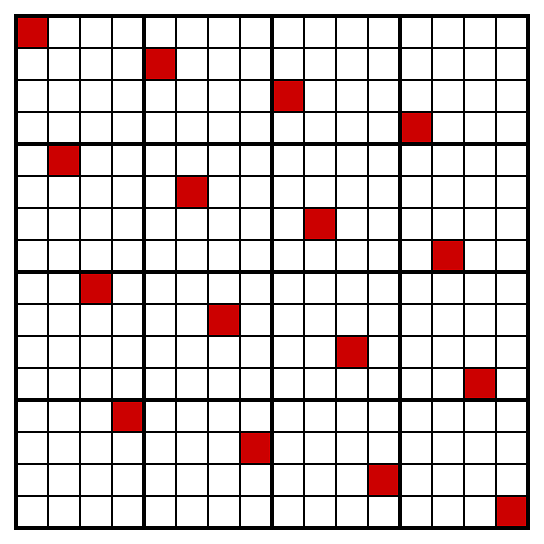
\includegraphics[width=7cm]{media/rooks.png}
\end{center}

To show that this works, consider for each rook drawing an $m \times m$ square of $X$'s whose bottom-right hand corner is the rook (these may go off the board). These indicate positions where one cannot place the upper-left hand corner of any square. It's easy to see that these cover the entire board, except parts of the last $m-1$ columns, which don't matter anyways.

Finally, to hit $n \le m^2$, just delete a row/column, and then if necessary place a rook in the unique position that fills the gap.


\section{Problem 3}
\begin{center}
\begin{asy}
pair A = dir(110);
pair B = dir(200);
pair D = dir(-20);
pair C = -A;
pair H = foot(A, B, D);
pair Cs = -C+2*foot(origin, H, C);
pair As = -A+2*foot(origin, A, H);

filldraw(unitcircle, opacity(0.1)+lightcyan, lightblue);
draw(A--B--C--D--cycle, lightblue);

pair M = midpoint(B--As);
pair N = midpoint(D--As);

pair U = IP(Cs--N, circumcircle(D, H, As));
pair V = IP(Cs--M, circumcircle(B, H, As));
pair Ss = D+As-U;
pair Ts = B+As-V;
pair T = extension(Ts, H, A, D);
pair S = extension(Ss, H, A, B);

pair O_D = circumcenter(C, H, T);

filldraw(circumcircle(C, H, T), opacity(0.1)+yellow, red);
pair P = extension(A, H, O_D, midpoint(T--H));
draw(A--H, lightblue);
draw(B--D, lightblue);

draw(H--C--T--cycle, red);
draw(H--O_D, lightblue);
draw(P--O_D, heavygreen);

dot("$A$", A, dir(A));
dot("$B$", B, dir(B));
dot("$D$", D, dir(D));
dot("$C$", C, dir(C));
dot("$H$", H, dir(H));
dot("$T$", T, dir(80));
dot("$S$", S, dir(S));
dot("$O_D$", O_D, dir(45));
dot("$P$", P, dir(45));
\end{asy}
\end{center}

First by angle chasing one can show that $\angle ATH = \angle TCH + 90^{\circ}$, so the tangent to $(CHT)$ at $T$ is perpendicular to $\ol{AD}$.
Thus the circumcenter $O$ of $\triangle TCH$ lies on $\ol{AD}$.

Let the perpendicular bisector of $\ol{TH}$ meet $\ol{AH}$ at $P$ now.
It suffices to show that $\frac{AP}{PH}$ is symmetric in $b = AD$ and $d=AB$, because then $P$ will be the circumcenter of $\triangle
TSH$. To do this, set $AH = \frac{bd}{2R}$ and $AC=2R$.
Use the Law of Cosines on $\triangle ACO$ and $\triangle AHO$, using variables $x=AO$ and $r=HO$.  We get that
\[ r^2 = x^2 + AH^2 - 2x \cdot AH \cdot \frac{d}{2R} = x^2 + (2R)^2 - 2bx. \]
By the Angle Bisector Theorem, $\frac{AP}{PH} = \frac{AO}{HO}$. Hence we just need to show $\frac{r^2}{x^2}$ is symmetric in $b$ and $d$.

Notice that \[ r^2 - x^2 = h^2 - 2xh \cdot \frac{d}{2R} = (2R)^2 - 2bx \] where $h = AH = \frac{bd}{2R}$, whence \[
x = \frac{(2R)^2-h^2}{2b - 2h \cdot \frac{d}{2R}}.
\] Moreover, \[
  \frac{1}{2} \left(  \frac{r^2}{x^2}-1 \right) = \frac{1}{x} \left( \frac 2x R^2 - b \right).
\]
Now, if we plug in the $x$ in the right-hand side of the above, we obtain
\[ \frac{2b-2h \cdot \frac{d}{2R}}{4R^2-h^2}
  \left( \frac{2b-2h \cdot \frac{d}{2R}}{4R^2-h^2} \cdot 2R^2 - b\right)
  = \frac{2h}{(4R^2-h^2)^2}
  \left( b- h \cdot \frac{d}{2R} \right)
  \left( -2hdR + bh^2  \right). \]
Pulling out a factor of $-2Rh$ from the rightmost term, we get something that is symmetric in $b$ and $d$, as required.



\section{Problem 4}
Since $PB = c^2/a$ we have $P = (0 : a^2-c^2 : c^2)$, so $M = (-a^2 : {--} : 2c^2)$. Similarly $N = (-a^2 : 2b^2 : {--})$. Thus
\[ \overline{BM} \cap \overline{CN} = (-a^2 : 2b^2 : 2c^2) \]
which clearly lies on the circumcircle.


\section{Problem 5}
We'll prove the result for at most $k - \tfrac 12$ with $k$ groups.
First, perform the following optimizations.
\begin{itemize}
  \ii If any coin of size $\frac{1}{2m}$ appears twice, then replace it with a single coin of size $\frac{1}{m}$.
  \ii If any coin of size $\frac{1}{2m+1}$ appears $2m+1$ times, group it into a single group and induct downwards.
\end{itemize}
Apply this operation repeatedly until it cannot be done anymore.

Now construct boxes $B_0$, $B_1$, \dots, $B_{k-1}$.  In box $B_0$ put any coins of size $\tfrac 12$ (clearly there is at most one).
In the other boxes $B_m$, put coins of size $\frac{1}{2m+1}$ and $\frac{1}{2m+2}$ (at most $2m$ of the former and at most one of the latter).
Note that the total weight in the box is less than $1$.
Finally, place the remaining ``light'' coins of size at most $\frac{1}{2k+1}$ in a pile.

Then just toss coins from the pile into the boxes arbitrarily, other than the proviso that no box should have its weight exceed $1$.
We claim this uses up all coins in the pile. Assume not, and that some coin remains in the pile when all the boxes are saturated.
Then all the boxes must have at least $1 -\frac{1}{2k+1}$, meaning the total amount in the boxes is strictly greater than
\[ k \left( 1 - \frac{1}{2k+1} \right) > k - \tfrac 12 \]
which is a contradiction. This gets a stronger bound $k - \frac{k}{2k+1}$ than the requested $k-\tfrac 12$.

And dear IMO jury: THIS IS NOT A NUMBER THEORY PROBLEM.


\section{Problem 6}
Let $c = (6e)^{-\frac12}$. We'll show the bound $c \sqrt n$.

The main core of the proof is the following lemma.
\begin{lemma*}[Lovasz Local Lemma]
  Consider several events, each occurring with probability at most $p$, such that
  each event is depends on at most $d$ of the others. If \[ epd \le 1 \]
  then there is a nonzero probability that no events happen.
\end{lemma*}
Split the $n$ lines into $c \sqrt n$ groups of size $\frac{\sqrt n}{c}$ each, arbitrarily.
We are going to select one line from each of the groups at random to be blue.
For each of the regions $R_1$, $R_2$, \dots, $R_m$ we will consider an event $A_k$ meaning ``three of the lines bounding $R_k$ are blue'';
we designate these lines beforehand.
We will show there is a nonzero probability that no events occur.

The probability of $A_k$ is clearly at most $\left( \frac{c}{\sqrt n} \right)^3$.

For each $R_k$, we have three groups to consider. Each group consists of $\frac{\sqrt n}{c}$ lines. Each line is part of at most $2n-2$ regions.
Hence $A_k$ depends on at most $3 \cdot \frac{\sqrt n}{c} \cdot (2n-2)$ events.

Thus,
\[ e \left( \frac{c}{\sqrt n} \right)^3 \left( 3 \cdot \frac{\sqrt{n}}{c} \cdot (2n-2) \right)
  < 6ec^2 = 1 \]
and we are done by LLL.


\section{Day 1 Contest Analysis}
I start with Problem 3 for the first ten minutes and lament the nonexistent diagram. I don't get very far other than drawing an okay picture and figuring out that the ``tangent to $BD$'' is just fancy for ``the circumcenter is on $AH$''.
I consider complex numbers but it seems to messy.
Thus I decide it's a good time to use the restroom and get some water.

When I return I decide to begin working on \#2, the combinatorics.
I bash out the cases for $n=1,2,3,4,5,6,7$ before deciding that this is getting annoying.
During this time I realize (by doing $n=5$) that when $n=m^2+1$ it's trivial to find an $m \times m$ bound.

At the time I don't think much of it and decide to go kill \#1, because it's been half an hour and I feel like I should probably get something done.
Basically I write the first thing that comes to mind nicely, and it works, because of course it works, because it's a \#1. I almost flip inequalities
a bunch of times but after half an hour of scribbling and crossing things out the problem is dead and I'm like okay.
This was in retrospect sub-optimal and I should have looked at least one specific case.
Not a big deal though, \#1 is \#1.

I then return to \#2 and look at $n=5$ again, musing that the bound $k=2$ was quite weak.
Then I realize $n=4$ has answer $k=1$.
Immediately I become convinced that the answer was just $\left\lfloor \sqrt{n-1} \right\rfloor$ and that the problem was merely
finding the necessary construction when $n=m^2$, because this was a \#2 and rooks are weird so there are not that many ways
the problem can end.
It takes about half an hour of fooling around to find said configuration -- it is a helpful hint that the $m^2 \times m^2$ can be
divided into a bunch of $m \times m$ sub-squares which each necessarily have a rook in them.
Once I find the configuration I breathe a sigh of relief knowing that I have two problems, the ``didn't fail'' threshold.
I now have three hours left to address the third question.
I use this opportunity to use the restroom again.

Since this is a \#3 geometry I would like to be looking at a diagram for things to prove are true, but the condition is really rather annoying.
It takes me almost an hour to realize that in fact the circumcenter of $\triangle TCH$ lies on $AD$ -- I finally realized this when blindly
angle chasing and looking for things that are cyclic when I noticed that the tangent to $(TCH)$ at $T$ was a line perpendicular to $AD$.
Suddenly I can actually draw the diagram.

Except at this point I have the urge to bash. Specifically, I just have to show that the perpendicular bisector of $HT$ meets $AH$ in the same place, meaning I have to show $PH$ depends is symmetric in $b$, $d$, where $P$ was the intersection.
And FOR THE FIRST TIME IN FOREVER, the Law of Cosines looks like a good option.
I'm hesitant to use it since I have never ever used the Law of Cosines in an olympiad before, and the IMO is a sub-optimal time to try a technique for the first time.

But it just looked too nice: let $x=AO$, $h = AH$, $d=AB$, $b=AD$, $R = \half AC$, and $r=HO=CO=TO$, where $O$ is the circumcenter of $\triangle THC$.  Then
\[ r^2 = h^2 + x^2 - 2xh \frac{d}{2R}
  = (2R)^2 + x^2 - 2(2R)h \frac{b}{2R}. \]
Here $h = \frac{1}{2R} bd$. Subtracting the two equations cancels off the $r^2$ and $x^2$, giving us a linear equation to quickly find $x$.

I wasn't sure how to pin down $PH$, though. My first impression was to use $x$ to compute $r$, then find $AT = x-r$, and then do some computations. I had planned to use a homothety with ratio $2$ at $H$ to compute $P'$, the point on $AH$ such that $\angle P'TH = 90\dg$.
These computations quickly get hairy and I don't actually want to do them.
Most importantly, I really did not want to evaluate $\sqrt r$.

I spend another 30-60 minutes slogging around rather lost, constantly wavering between trying to find a better bash and going for the all-out slog with the time remaining,  until I finally realize that
\[ \frac{AP}{PH} = \frac{AH}{OH} = \frac{x}{r} \]
by the Angle Bisector Theorem. And so I just had to show this was symmetric, but
\[ \frac{r^2}{x^2} = 1 + \frac{(2R)^2}{x^2} - \frac{2bh}{x}. \]
You can tell by looking now that this should be really direct to compute. It shouldn't take more than 15 minutes by any contestant in the room, and shouldn't take more than 10 for a seasoned basher like me.
But the pressure of the IMO sets in around now, and I repeatedly miscomputed for the next while.

Sitting at the edge of getting an IMO3, I become so nervous that I begin visibly shaking.
I have around 70-90 minutes left, which I tell myself is more than enough.
I go to use the bathroom and come back no longer shaking -- standing up does wonders for this sort of thing.
I then re-start the bash from scratch and finish in 10 minutes.

Well\dots done with the IMO an hour early. What do you know?

I consider walking out early since I probably will never have a chance to say ``I walked out of the IMO early'' ever again, but decide against it since it's a rather mean to the other contestants.
I neatly collate my solutions and the scratch work into the problem folders. It probably was not necessary to include my failed diagrams and random wrong calculations in \#3, or any of the other problems for that matter, but I did it just in case anyways.
This inflated my four-page solution to \#3 to seventeen pages of script.

I eat a little bit of chocolate and then decide it's an excellent time to start drawing random pictures to add to the end of my solutions.
I draw a scene of a large chessboard with rooks and peace signs hanging out in distinct rows and columns, and then another picture of a dinosaur labelled $a_{2014}$ chasing after some other terms of the sequence $(a_n)$, and so on.
One of the invigilators notices me doing this and laughs.

Well, whatever. Just have to stay calm for Day 2.

\section{Day 2 Contest Analysis}
First I incinerate \#4 with barycentric coordinates.  Cool.

Then I get stuck on \#5 for three hours. It is really very slippery; there are too many things to try that do not work.
The greedy algorithm in fact fails if applied directly and some optimization is needed.
I begin the problem with an optimization of switching $\frac{1}{km} \times k$ with $\frac{1}{m}$, limiting the number of times each coin appears,
and in particular making even-numbered coins appear at most once.
I also remove any $1$'s that show up as this occurs, since one can just induct down ($99$ is just a random number, clearly\dots).
But it takes forever and a half until I find the construction; I finally noticed it while staring at the row of numbers
\[ \half \qquad \frac 13 \times 2 \quad \frac 14 \qquad \frac 15 \times 4 \quad \frac 1 6 \qquad \dots \]
and realizing I could get $k$ bins and a bunch of small $\frac{1}{2k}$ coins.
I had been playing with the $\frac{1}{2k}$ coins idea but had approached it from the wrong angle of a stronger induction hypothesis.

So anyways I end up with just about an hour for the final problem.
Miraculously fooling around with LLL gets me a $c>0$. Well. Okay.

GCC'ed again!

\chapter{Diary of Events}
\section{July 5 -- The Airplane Ride}
I'm designated the official camera-wielder for the trip based on my prolific picture-taking during the camps.

\begin{figure}[ht]
  \centering
  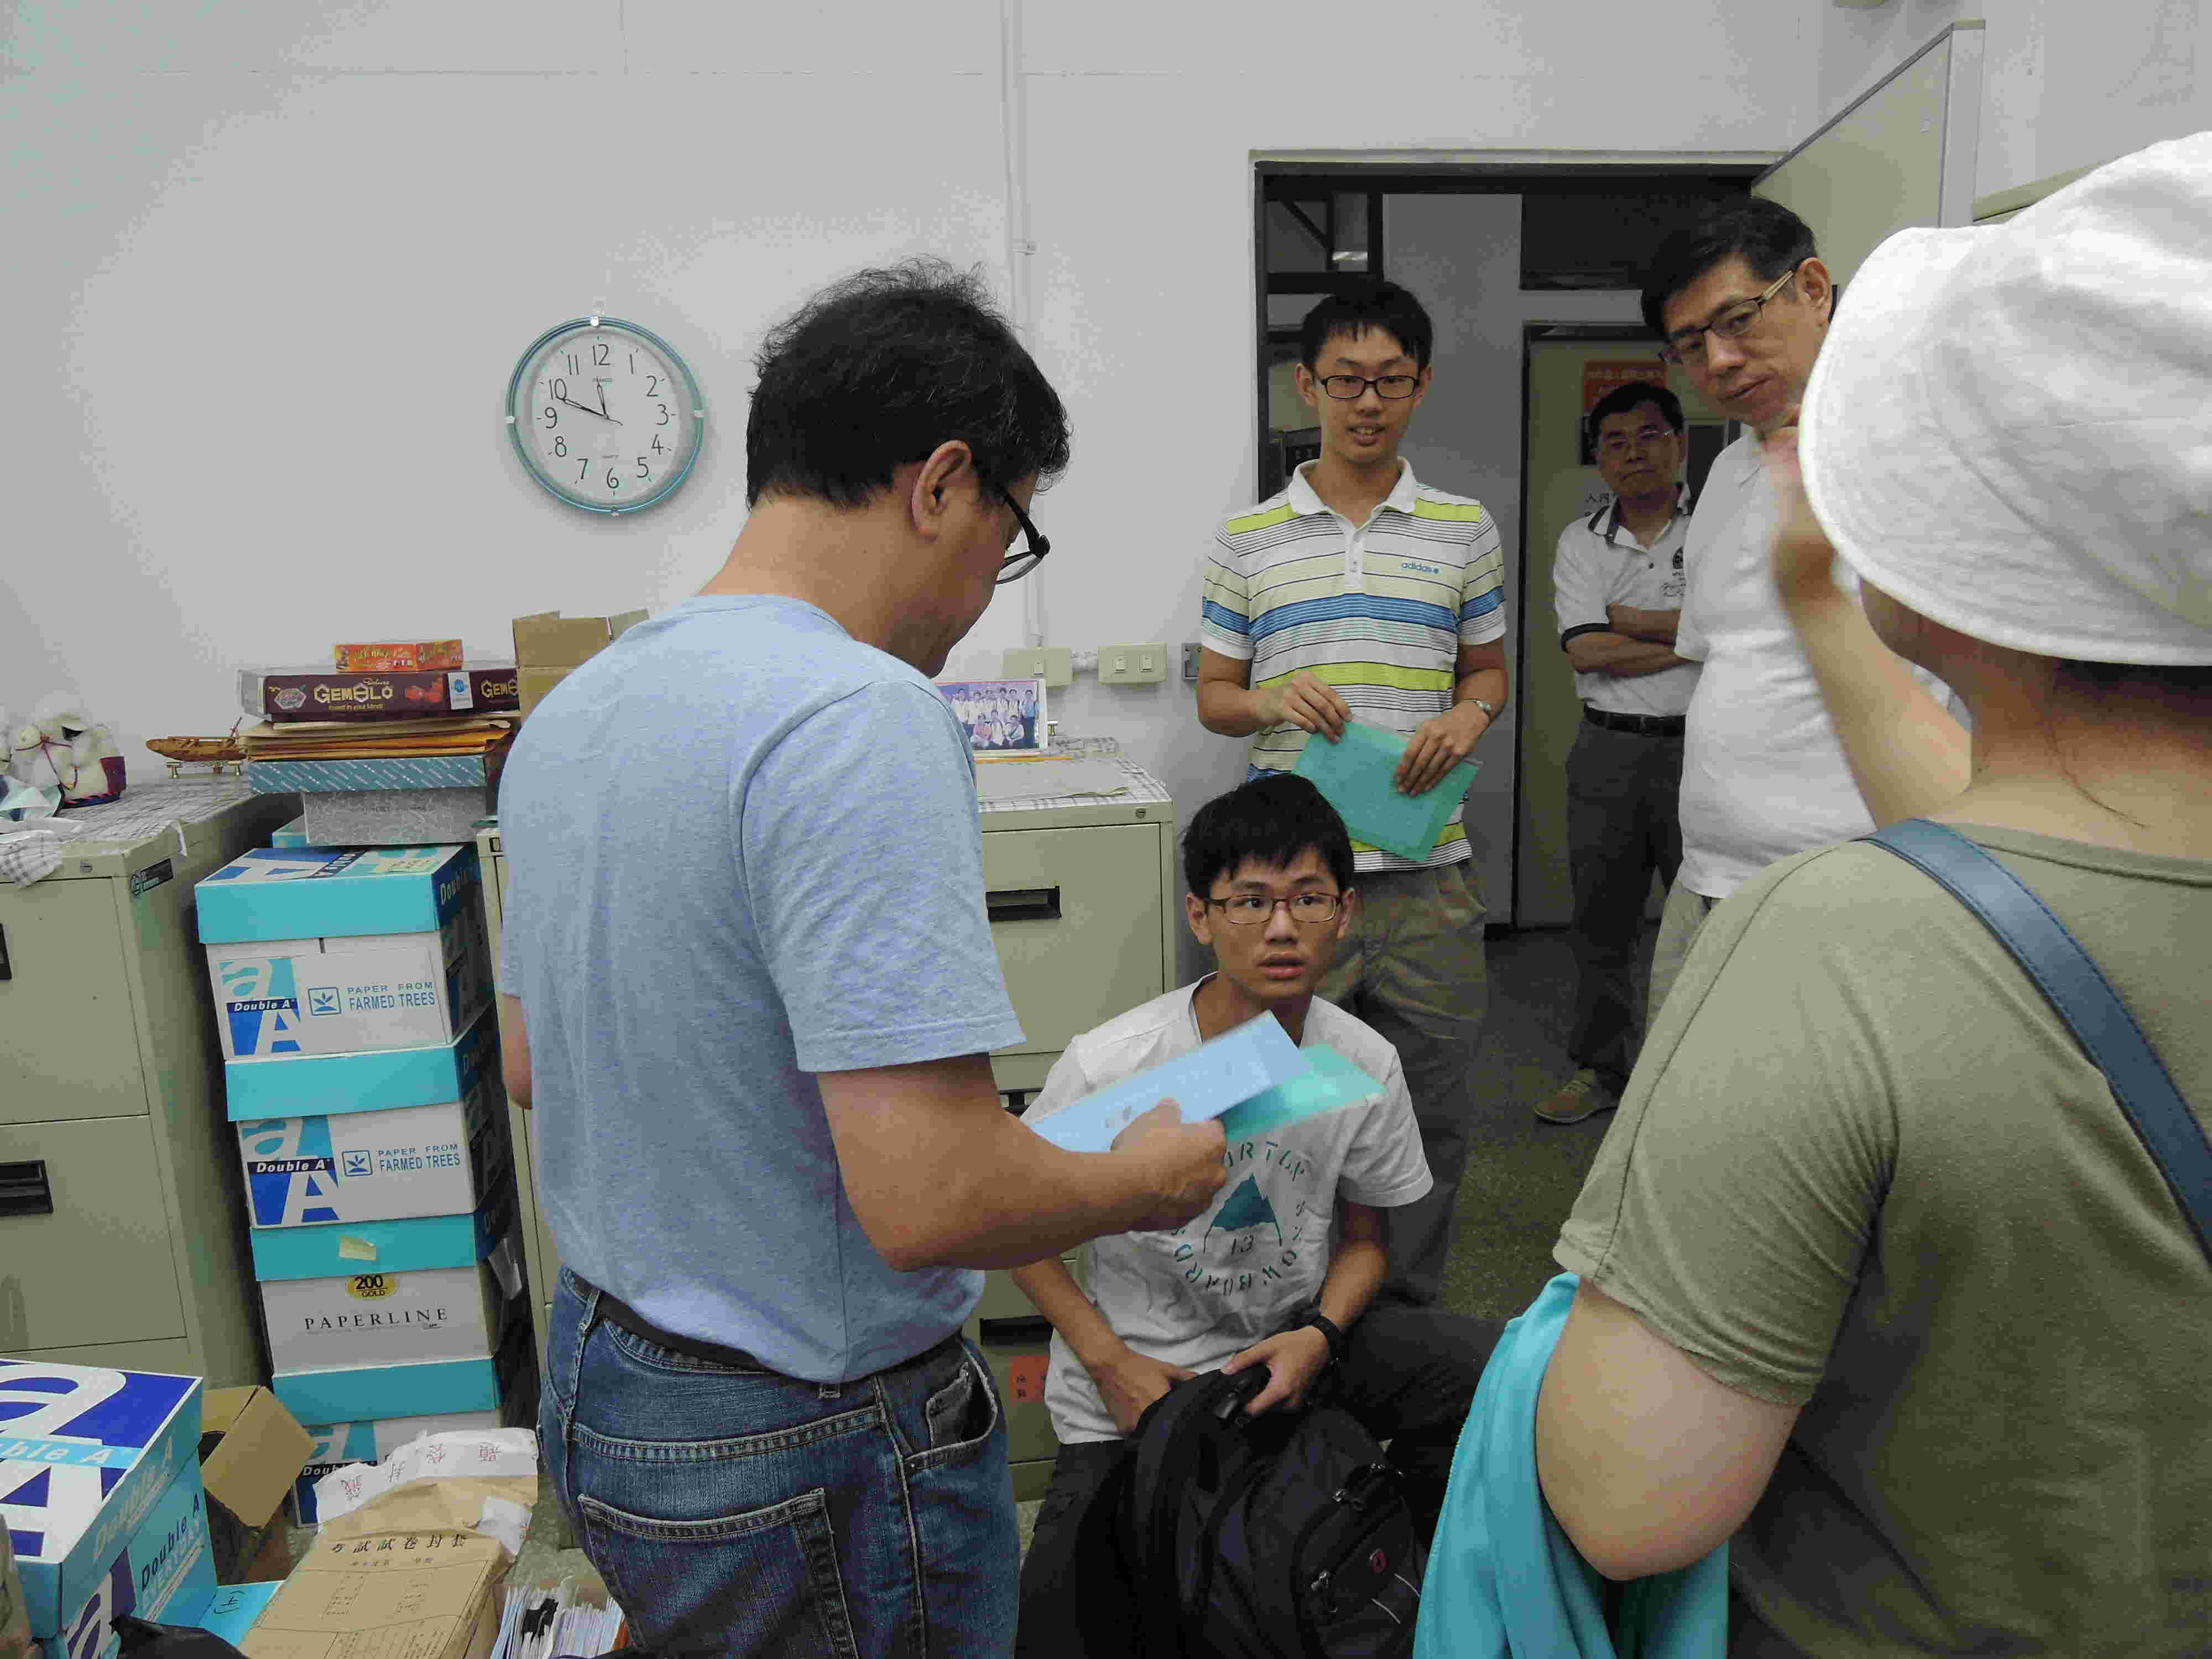
\includegraphics[width=0.5\textwidth]{media/first.jpg}
  \caption{Inaugural camera photo.}
\end{figure}

Over the ride to the IMO, we take great pleasure in ``discussing'' inequalities:
\begin{quote}
  甲:移過去就直接炸啊 \\
  乙:炸完再怎樣 \\
  甲:就 SOS 啊
\end{quote}
(The Chinese equivalent of ``bash'' is 「炸」, which means ``bomb'', so we were mostly making fun of airport security).

I mostly sleep through both plane rides. CBD spends the time watching Black Bullet, which I made the mistake of almost
finishing the couple days before the trip; this probably explains why I slept as much as I did.
During the layover at Singapore we see the China, Japan, Philippine, and Singapore teams, and get pictures with
the former two. I remember distinctly that during the picture with the China, one of the Taiwan members told another that
``picture-taking is part of the international experience'', to which one of the Chinese team members joked ``you mean
intra-national, right?''. Most of us (including me) laugh it off but it surprised me how politics was still well
and alive here.

I'm also amused by a large ``T2'' terminal number that shows up.

\begin{figure}[ht]
  \centering
  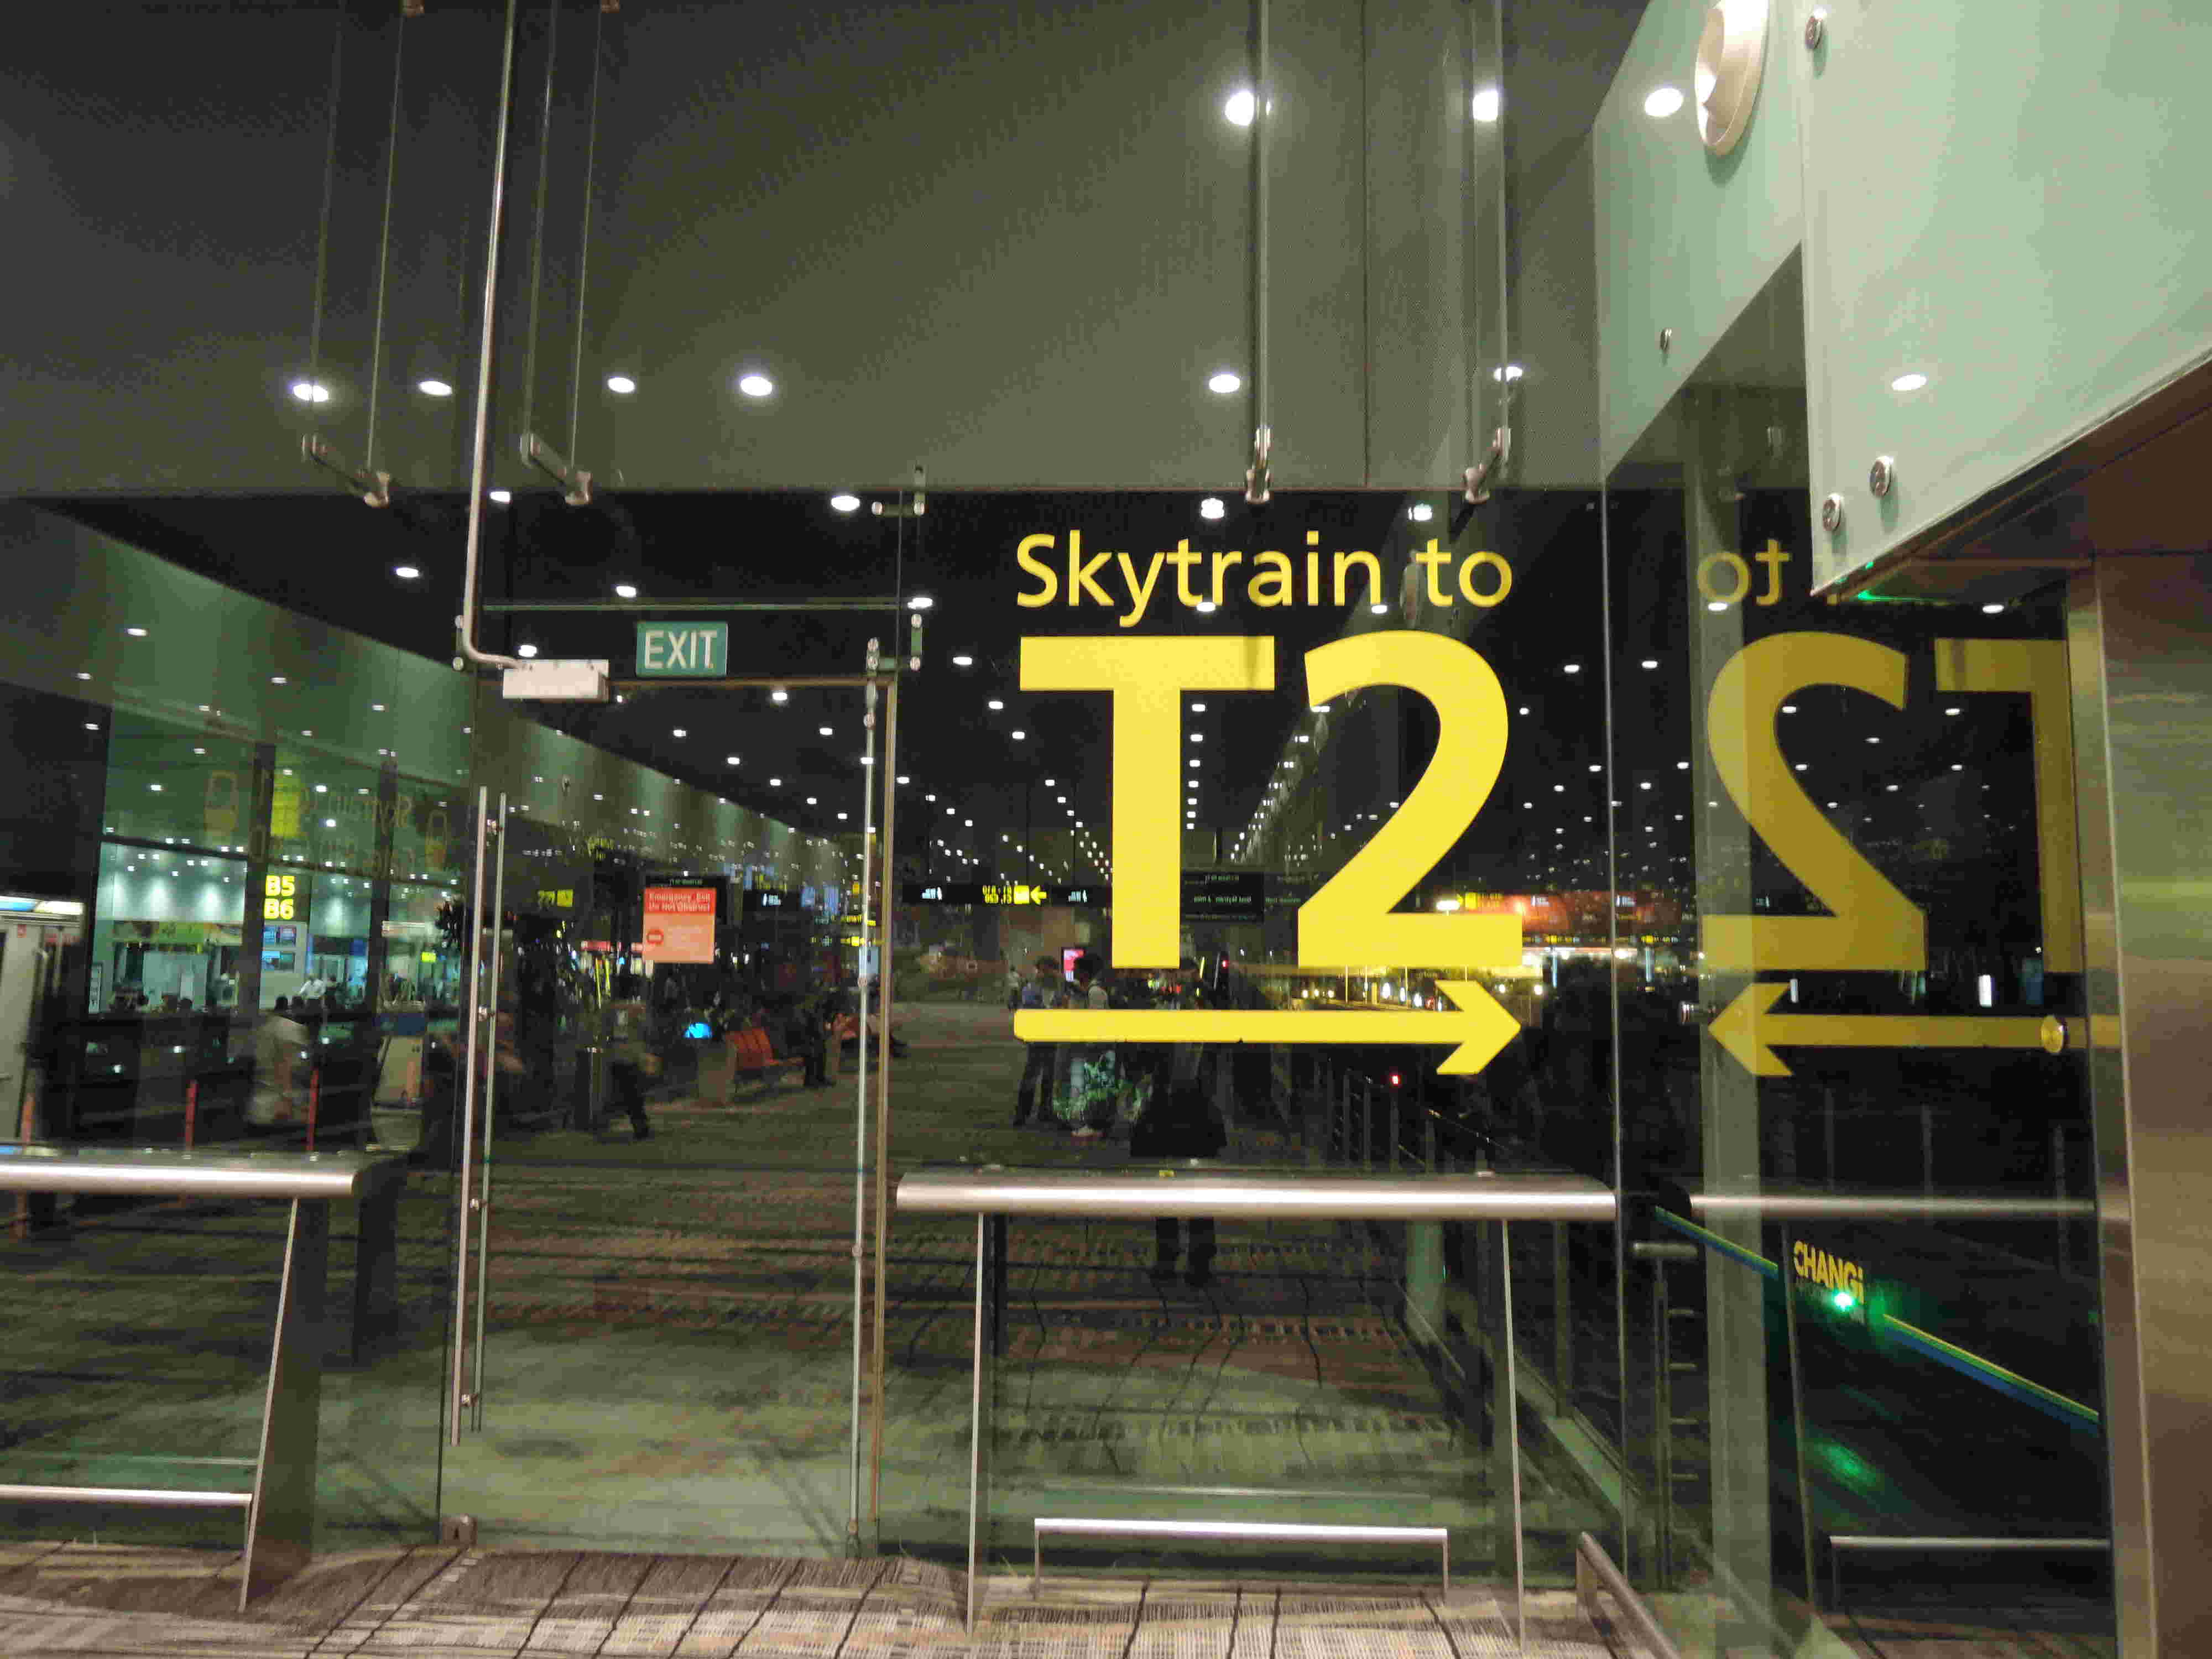
\includegraphics[width=0.5\textwidth]{media/T2.jpg}
  \caption{The Titu Terminal.}
\end{figure}


\section{July 6 -- Arrival}
We arrive at the Cape Town airport and Ting-Wei immediately tries to obtain Wi-Fi.
I am highly amused to find that the Wi-Fi registration requires email confirmation.
Someone has clearly never read Catch-22.

After passing customs are greeted by Amelia, our guide for the duration of the IMO.
It is odd to hear someone speaking English for the first time in roughly a month.
The rest of Taiwan tries to communicate to Amelia in rather broken English.
I become designated as the official translator for the team.

After a wait and the purchasing of several adapters, we board a bus.
During the bus ride, Ting-Wei and Hung-Hsun have a good time trolling some of the other bus
contestants with the following problems: fill in the blanks to form a math term.
\begin{enumerate}
  \ii \verb+*a*a*a*a+
  \ii \verb+*i*i*i*i*i**+
\end{enumerate}
They seem impressed when the Italian team responds within ten minutes.

\begin{figure}[ht]
  \centering
  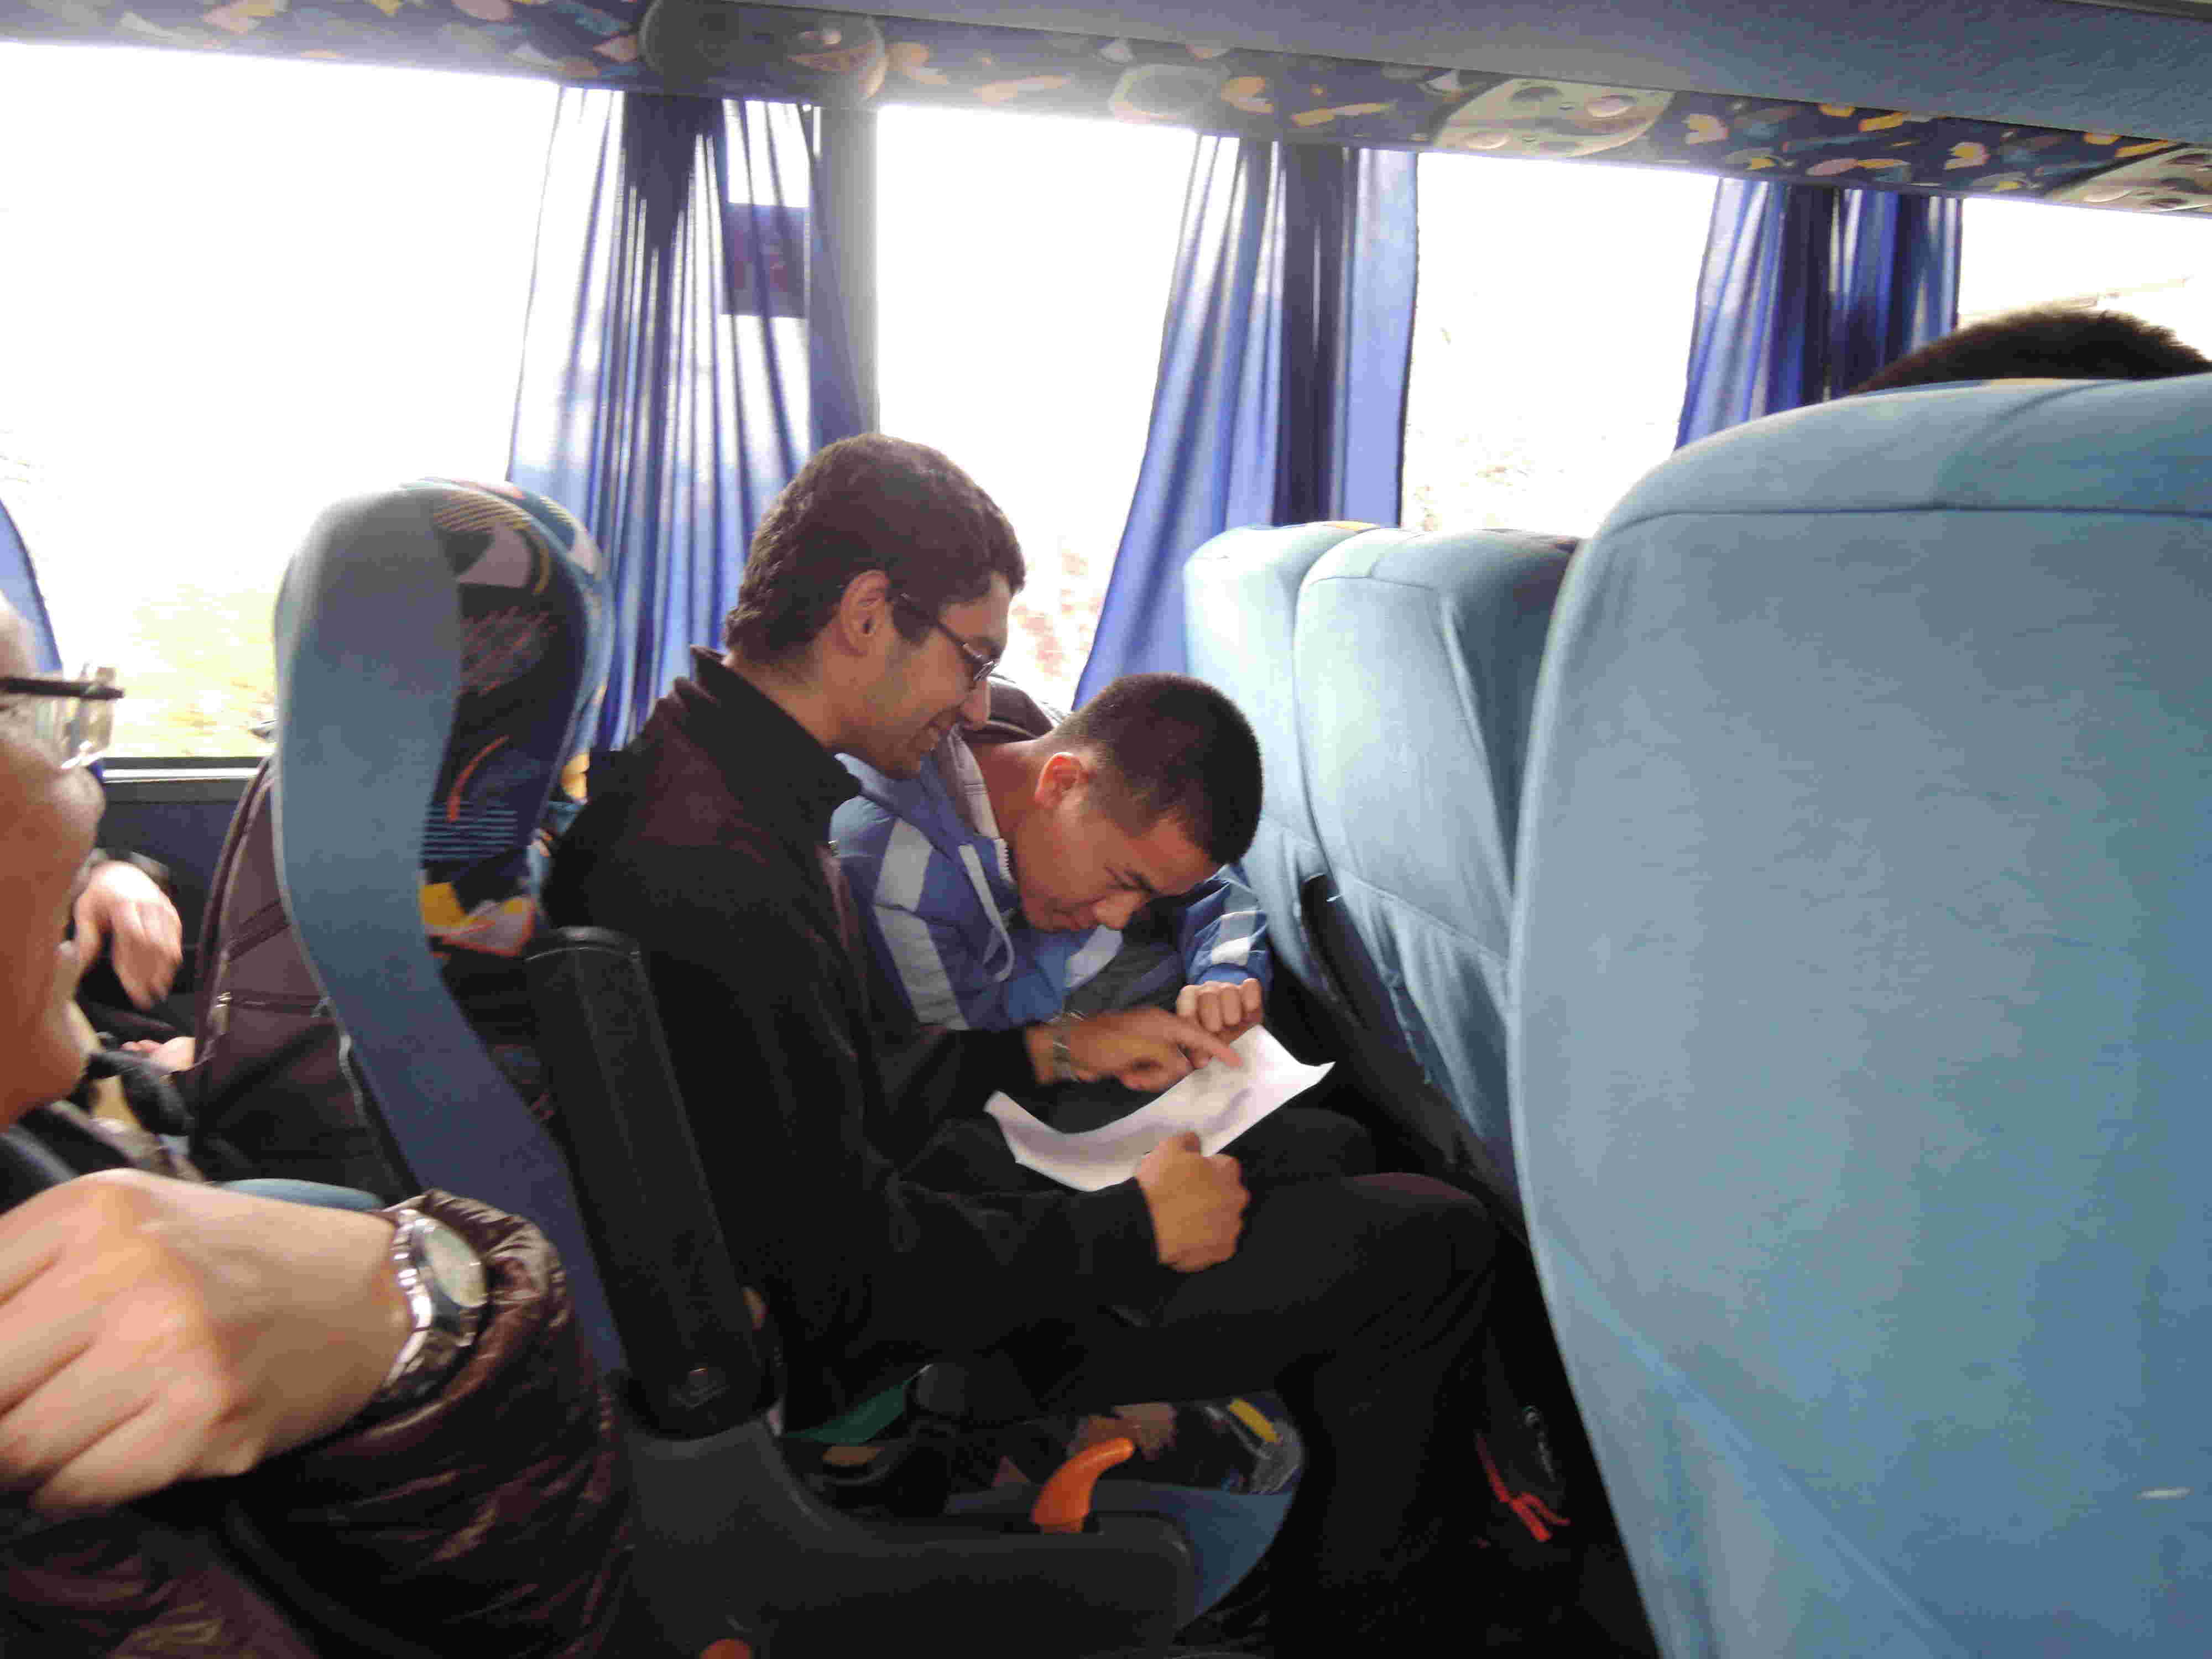
\includegraphics[width=0.5\textwidth]{media/bus_troll_problem.jpg}
  \caption{People work on filling in blanks.}
\end{figure}

Another wait rewards us with several hats, a jacket, and a bag with goodies inside.
We then head over to get back to our dorms, hoping for the promised WiFi, as none of us have had Internet
for many several hours. Our deputy leader tells us to be back by 12:40PM to go to lunch.

It's at this point that we get the first logistical troubles.
We get shoved into a small lobby with some other teams, and an imbecile is at a desk handing out keys.
The imbecile has two lists and insists to our tour guide that ``we are not in this building'' because we are
not one one of this lists, even though we are clearly on the other list, designated in Rooms 401-406, and
the keys are lying on the table. Nonetheless he refuses to give us the keys. Amelia calls for someone who
is apparently a superior in the IMO organization hierarchy, who comes and basically tells the imbecile he is an
idiot and to give us our keys. Unfortunately said superior takes his time to arrive, and so by the time the
imbecile hands us the keys it was 12:45. We hurry to our rooms, drop off our luggage, and rush down to find that
Dr.\ Hong is already waiting for us downstairs.

\begin{figure}[ht]
  \centering
  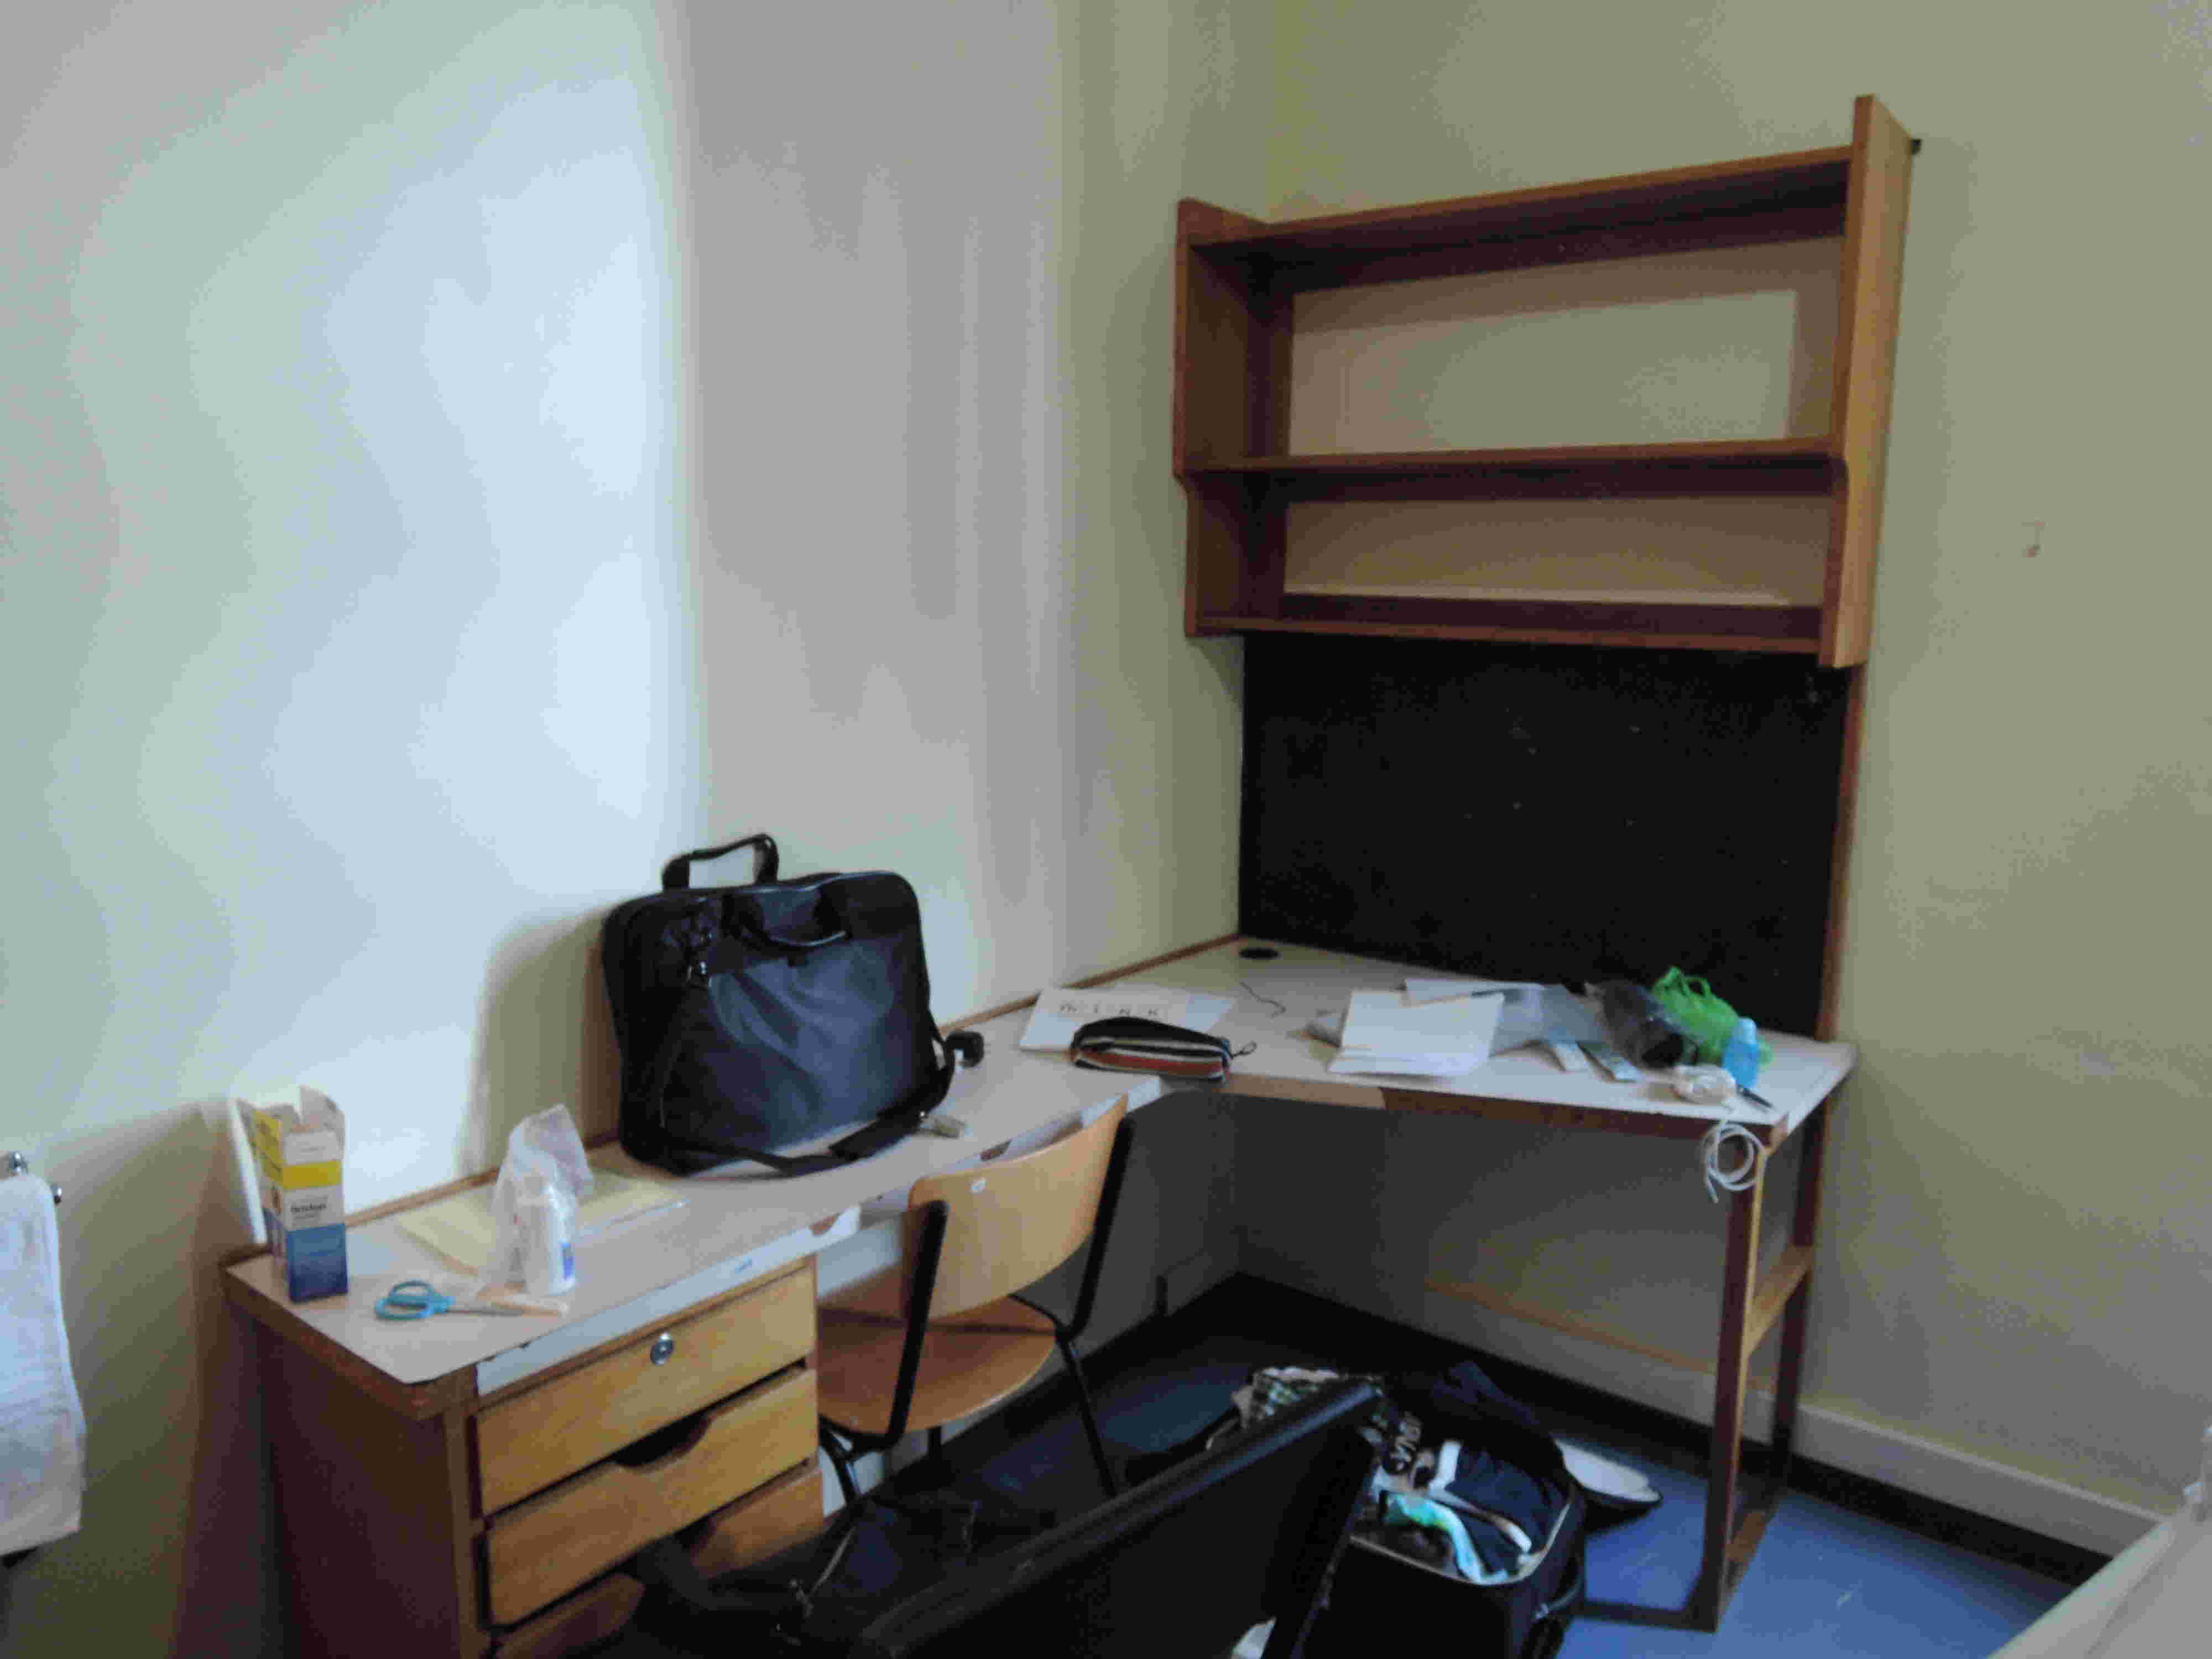
\includegraphics[width=0.5\textwidth]{media/room.jpg}
  \caption{My mess in Room 402.}
\end{figure}

After a totally forgettable lunch, we head with Dr.\ Hong and Dr.\ Hung to our rooms to properly asses the situation.
On the way back I briefly run into the Brazil team and wave to Victor Reis.
Upon returning to the dorm and beginning a proper observation,
\begin{enumerate}[(i)]
  \ii The rooms are in fact unheated, and only a single sheet has been provided.
  \ii None of the African adapters we brought work, and moreover the adapters we purchased at the airport
  successfully fit the Cape Town outlets on one end, but on the other end only accept European plugs.
  However, some of the Africa adapters we brought fit in the airport adapters, and so after much confusion
  the power issue is resolved in Room 406. As Room 406 is for some reason larger than the other rooms, we agree
  to all hang out in Room 406 whenever necessary.
  \ii There is no source of drinking water.
  \ii We cannot access WiFi (at least for the moment).
\end{enumerate}
It's also the case that the restrooms are external, like several college dorms.
There is a sink inside though, but the sink has two faucets, one which only dispenses hot water and one which
only dispenses cold water.  I bitterly remember that I will soon be stuck in a dorm in Boston as well.

Amelia goes to help us figure out the situation with the sheets.
Meanwhile, I am able to set up the adapters in my own room using toys that my dad had left me, and leave my
tablet and phone charging.
By this point it is about 2PM.
Po-Sheng indicates that last year the dorm situation was not this dismal.

CBD, Hung-Hsun, and Ting-Wei leave to obtain things for the supermarket with the teachers while the remaining IMO
contestants take a break in TWN6's room. I join them with my laptop (gradually running out of battery) and type
the first part of this report, while the Po-Sheng and Pang-Cheng play Candy Crush.
I then resort to playing Solitaire to pass the time.

The next several hours pass uneventfully, mostly consisting of me playing Solitaire while the rest of the Taiwan
team either does problems or plays Candy Crush. On the trip to dinner I run into a couple of people briefly,
namely the USA team, the Canada team, Livio Fetahu, and Victor Reis again.
The Canada team mentions their tap water is somewhat brown.

I finally manage to hijack Internet by borrowing a laptop plugged into a wired network and repeatedly ignoring password
prompts, so I respond to a buildup of emails and reminiscence of my times at MOP while the other contestants play Mao.
Finally at around 9PM our savior Amelia arrives with some rather thick blankets and tells us there is a game room in
the lobby that most of the other contestants are hanging out at. I resolve to check it out thoroughly the next day.
However, by this time I decide to retire to sleep.

\section{July 7 -- The Opening Ceremony}
I had planned to take a shower once the sun before we left for breakfast at 6:40AM, but find out the hard way
that the sun does not in fact rise until after 7AM.
So much for my shower.
Fortunately the bed had turned out to be sufficiently warm enough under three layers of thick blankets
while wearing sweatpants and my MIT jacket.

For breakfast I grab some muffin, cheese, and a bowl of cereal to which I add sugar.
After we eat breakfast, Amelia tells us that we will be going on a brief excursion at 9:00AM.
We decide to play some cards until excursion time.
Initially, Ting-Wei and Po-Sheng play an idiotic version of Yu-Gi-Oh crafted with playing cards.
We then decide to play less stupid games.
I am surprised to find that the rest of the Taiwan team in fact knows how to play Napoleon, albeit
with the following modifications:
\begin{itemize}
  \ii The two Jokers are included, one low Joker and one high Joker.
  They serve similar functions to the Secretary Card, in that they can be played at any time,
  are considered their own suit, and are higher than any other cards (other than the Sec card).
  However, they lose their powers after the first seven tricks.
  \ii As a result of the Jokers, the baggage now contains four cards.
  \ii The bids include the trump suit, in the style of Bridge.
  It is permissible to change the trump suit after seeing the Baggage at the cost
  of increasing the bid by $1$.
\end{itemize}
We also play Bridge and Big Two.

Our excursion takes us up to the top of a mountain, where I run into team USA again and converse
with them about the Shortlist. Evidently they felt that A6 was easy. Oops.
It's mentioned that Kevin Sun almost won Black MOP until he zero'd a day of the mock IMO consisting
of G2, A4, C6, which ironically I considered among the easiest problems in their corresponding categories.
The road to said mountain is quite steep and I nearly trip several times.

\begin{figure}[ht]
  \centering
  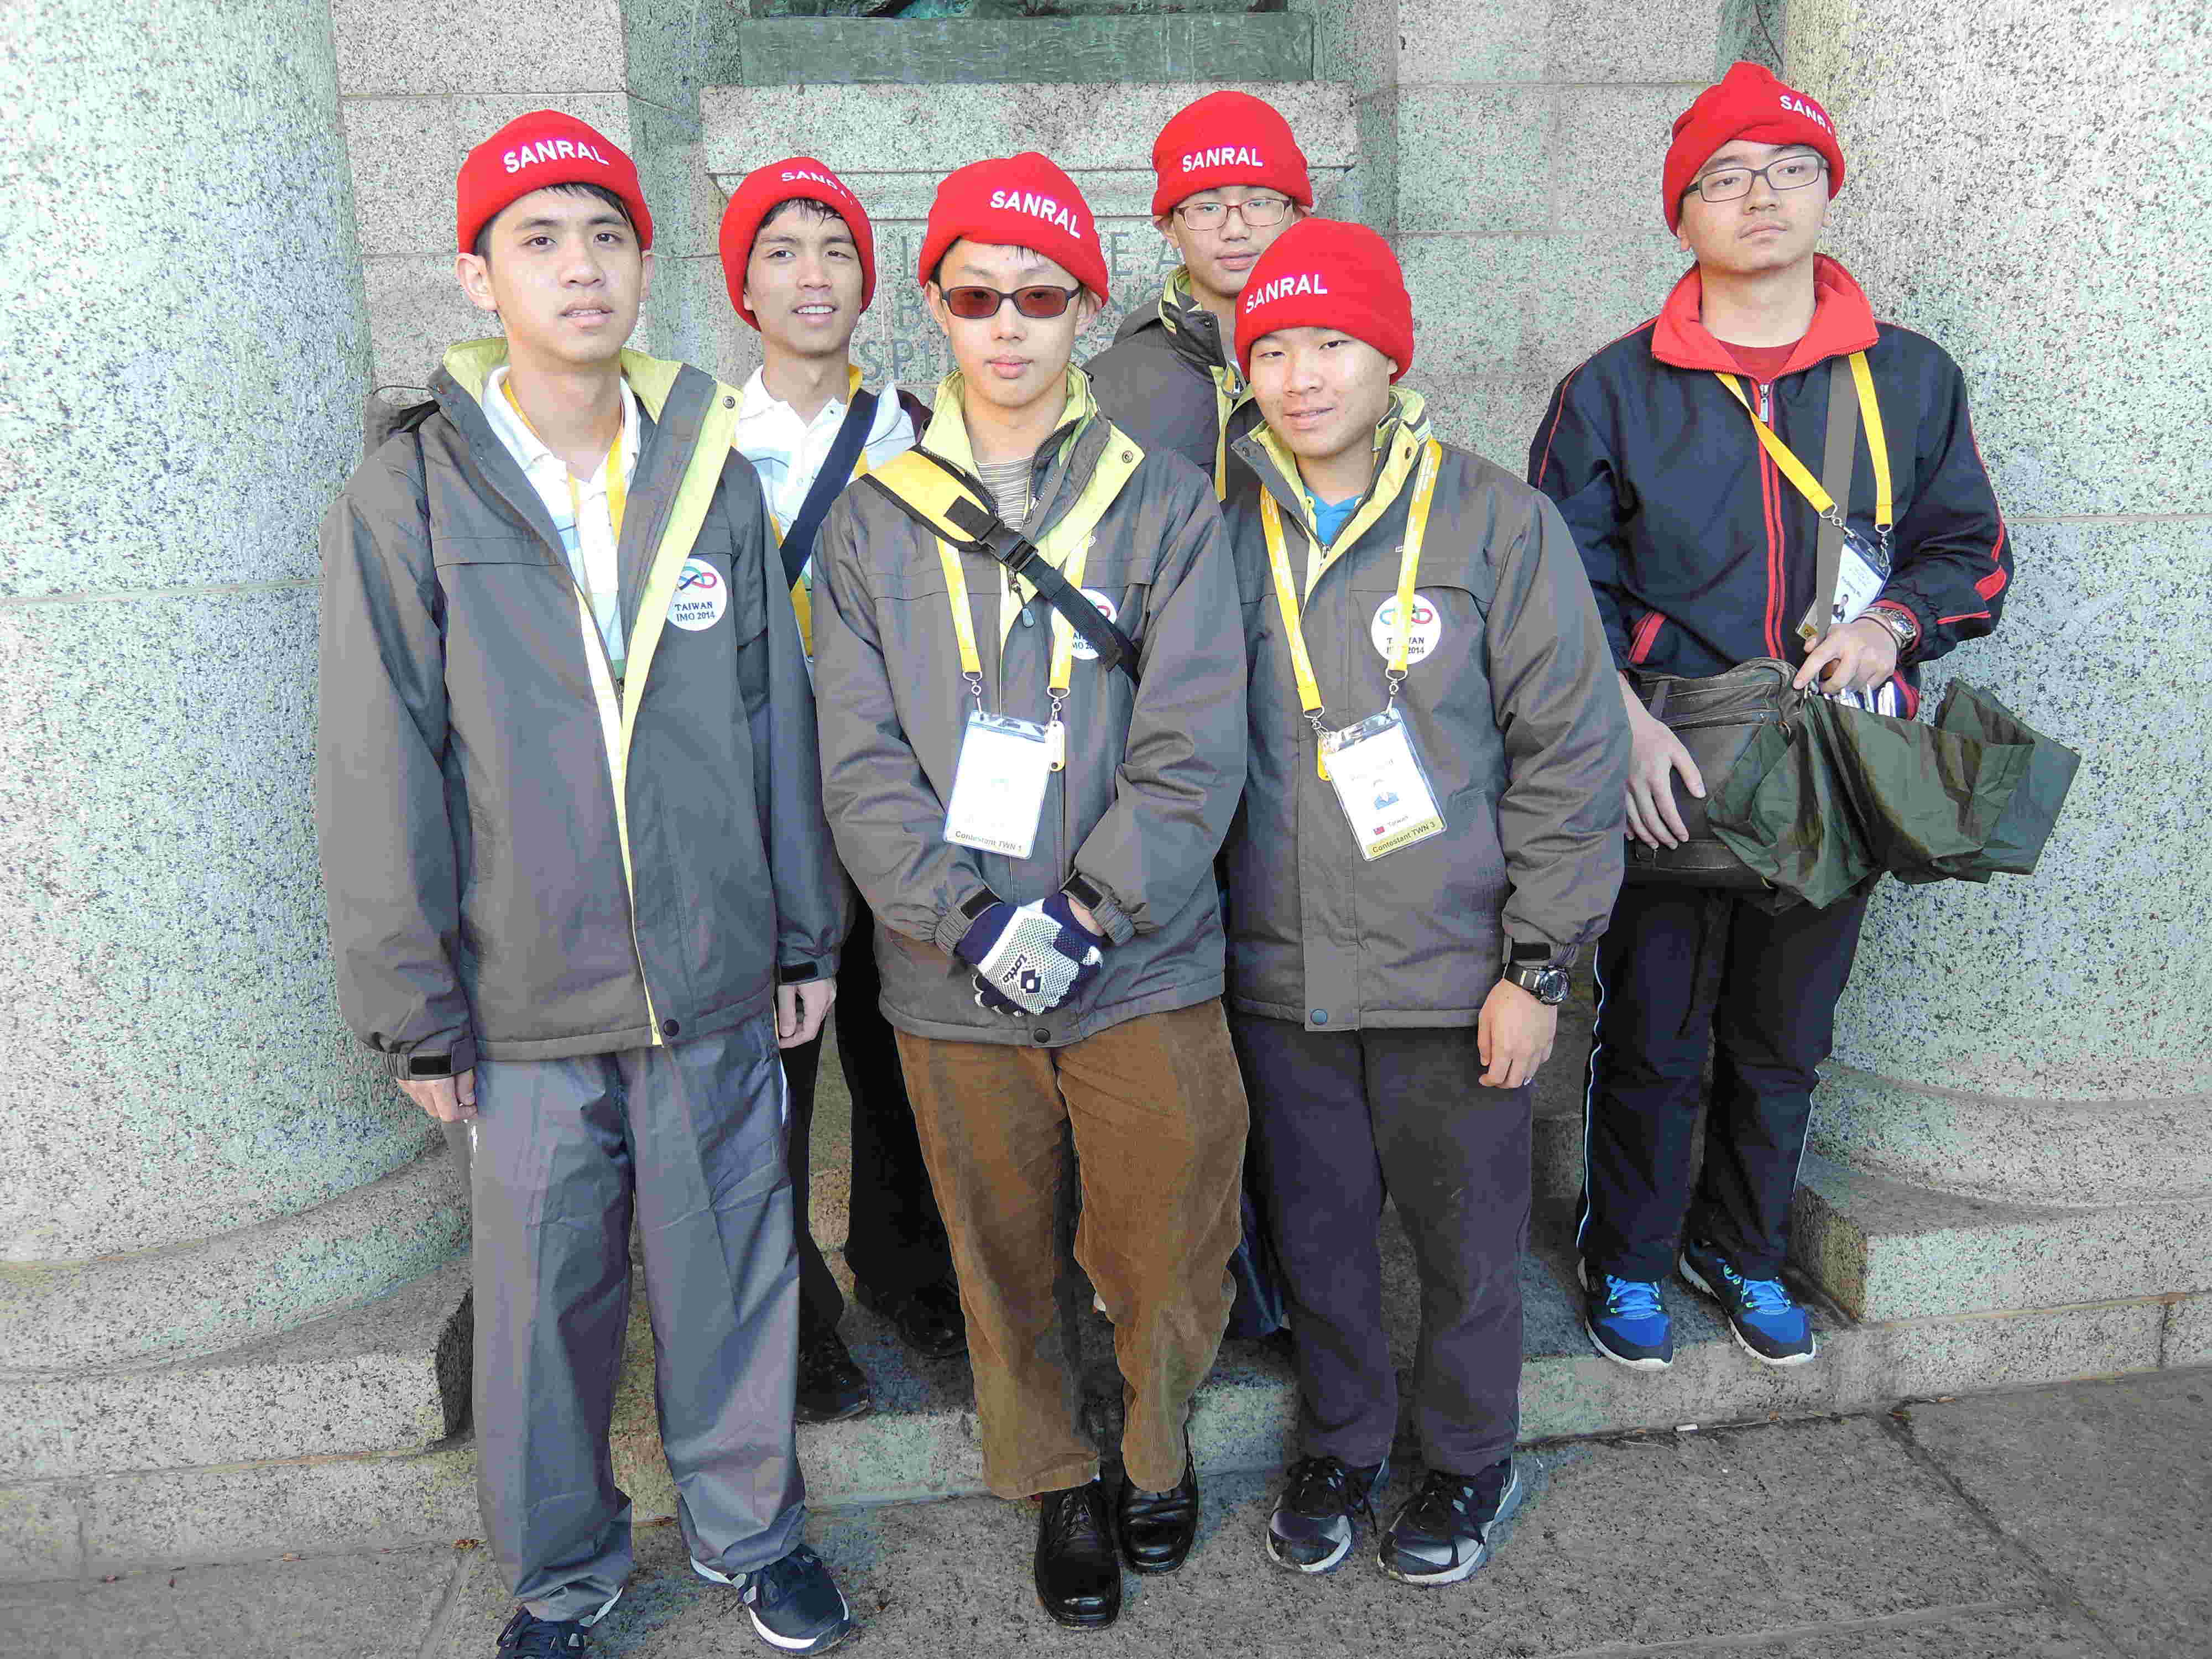
\includegraphics[width=0.5\textwidth]{media/mini_excursion.jpg}
  \caption{Near the top of the mountain.}
\end{figure}

We were planning to visit the city of Cape Town after the mountain, but the long waits for buses to take us
to various places throughout the campus lead us to decide to drop this part of the journey. Instead, Amelia
takes us to the site of the contest tomorrow -- a single large unheated gymnasium.
Seeing as there will be on the order of 500 students placed in one building tomorrow, I no longer feel
concerned about it being too cold.

Afterwards we return to the dining hall for lunch. Unlike the first dinner, the silverware has been properly
prepared this time. Moreover, we find that the butter is no longer wrapped but placed on a plastic-wrapped plate
in chunks, meaning that CBD will not mistake it for chocolate again. I take a tuna pasta dish.
After lunch we have a few hours to kill until the Opening Ceremony, so we play some games of Memory with the entire
54-card deck, which turns out to be very challenging, unless you happen to be the last player to move which essentially
gives you five or six pairs.
Then I teach the game Nertz, before the others decide it's a good idea to do more ELMO shortlist geometry.
I'm not in the mood for problems so I take out my laptop and update my diary up to that point.

The opening ceremony involves another bus ride -- quite unfortunate because the buses are clearly too small and we often have
to wait for a long period of time -- followed by waiting outside in the cold for approximately an hour. During this time we grab
a picture with the Hong Kong team, and witness a parade of team leaders who wave back towards the contestants. The team leaders
are quarantined from us until after the second day of the exam, so we will likely not see them again until then.
Ting-Wei remarks enthusiastically that Sen-Peng Eu and Roger Lin appear to be smiling, which means that we will do well.

\begin{figure}[ht]
  \centering
  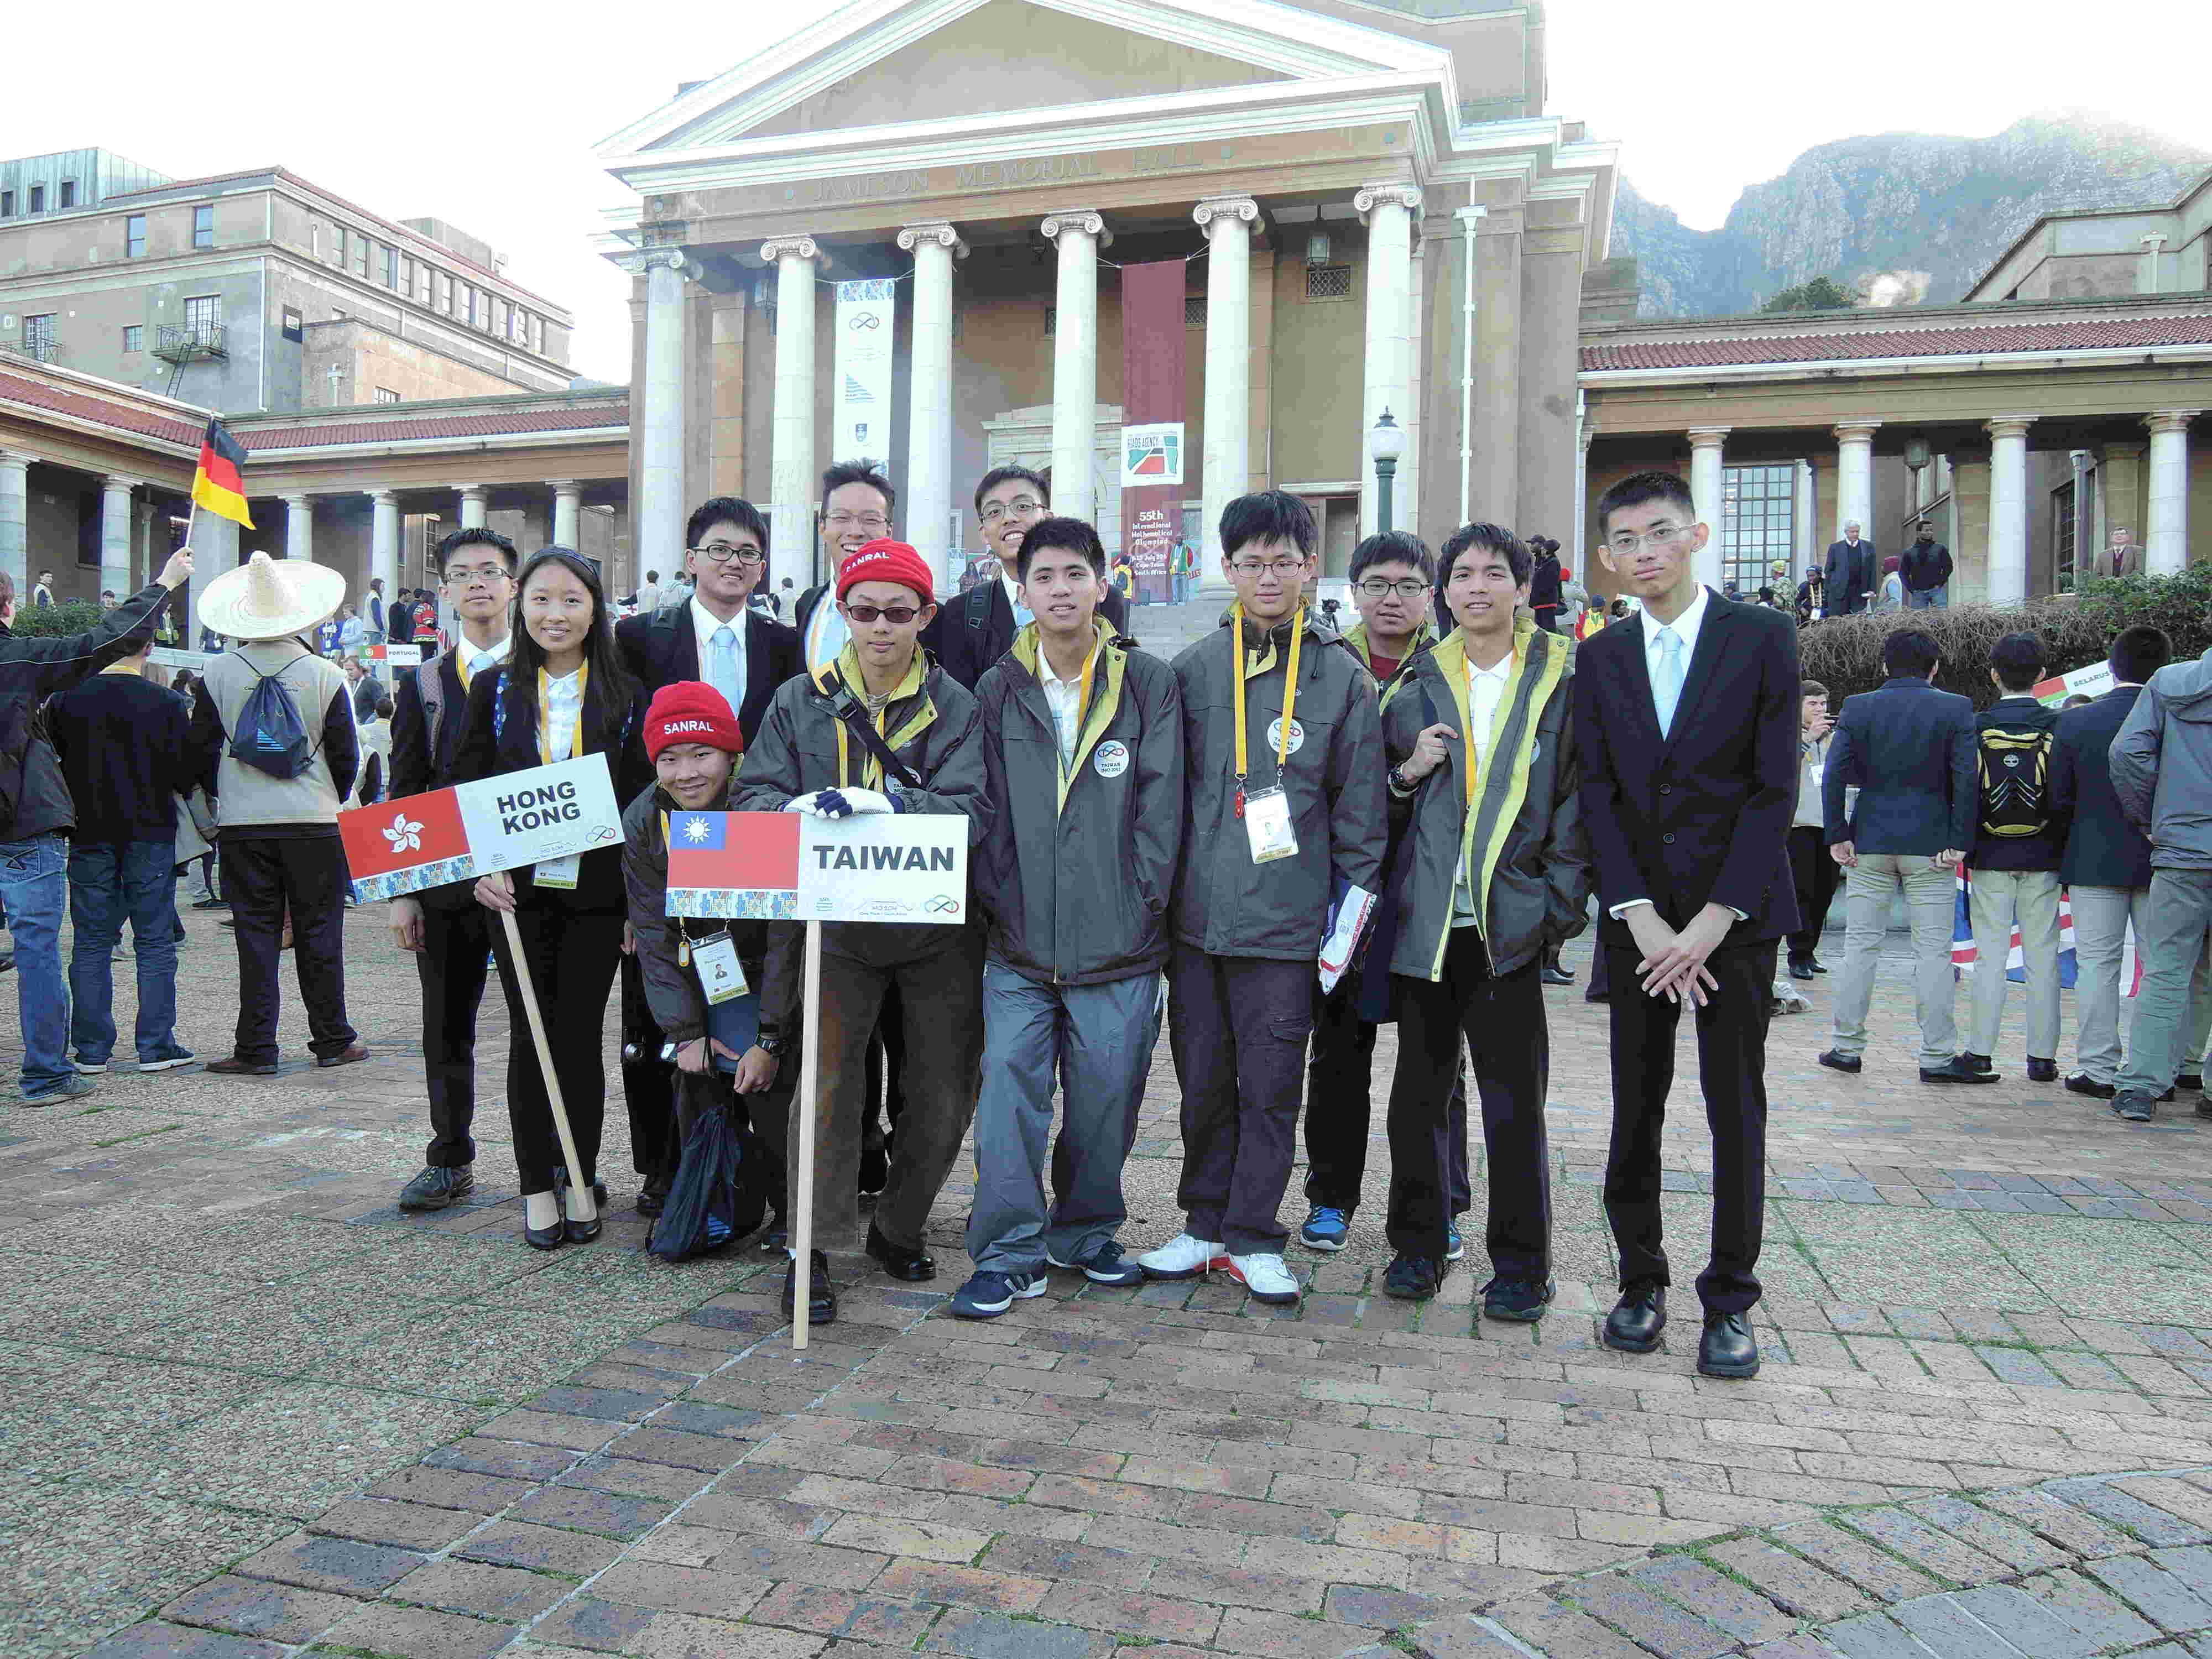
\includegraphics[width=0.5\textwidth]{media/hongkong_taiwan.jpg}
  \caption{Hong Kong and Taiwan teams.}
\end{figure}

For some reason the teams are gradually entered into the auditorium one by one; we are around 54th, just before South Africa,
so we enjoy some shivering in the cold for a while (about an hour) before we actually enter.
Quite unfortunately, we end up in the second-to-last row of the auditorium, where ``row'' refers to the rows of folding chairs
that were set up, making it quite impossible to actually see the stage.

The opening ceremony begins at 5:15 PM (15 minutes late)  with the national anthem, which is surprisingly long for a national anthem.
Then, the Vice Chancellor of the University of Cape Town (where the contest is hosted) makes a speech about how this is the
first time that the IMO has been held in Africa. He then goes on to make an ``Africa is not actually bad at math despite
what you might think'' style speech, going as far as to show us geological excavations which found a bone with 30 marks for
counting the days, and something else with parallel scratches on it, or something like that. The rest of the Taiwan team doesn't
actually understand what he is saying, meaning they are probably less bored than I am.

Similarly the minister of education makes his share of comments. I no longer remember what they are because around this point
a couple of birds decide to fly in through the back entrance and begin chirping, which thankfully provides some relief to speeches.
We then get a speech from someone from the Department of Roads (?) which I also no longer remember.

Subsequently, each of the countries goes up on the stage in the standard ritual, starting with Romania and proceeding in the order
that the countries joined the IMO. I end up translating a lot of the country names for CBD, who is sitting next to me.
The countries mostly stand and wave their flags, but some throw out goodies and one does a dance on the way.
A few countries have only one contestant, and the crowd gives massive applause to such countries (I'm not sure why).

In Taiwan's turn, we simply walk across the stage holding the flag. We are then immediately followed by South Africa, and
the host country makes a huge spectacle out of this with a band of percussion instruments for the next 20 minutes. Thankfully
this is the one time that we are in the front, having just gotten off the stage, so I can actually see what is happening.
The rhino from the airport joins the South African team in the parade.
Meanwhile, near the top of the ceiling some math formulae are projected.
I am dismayed to see the use of $^nC_k$ instead of $\binom nk$.

\begin{figure}[ht]
  \centering
  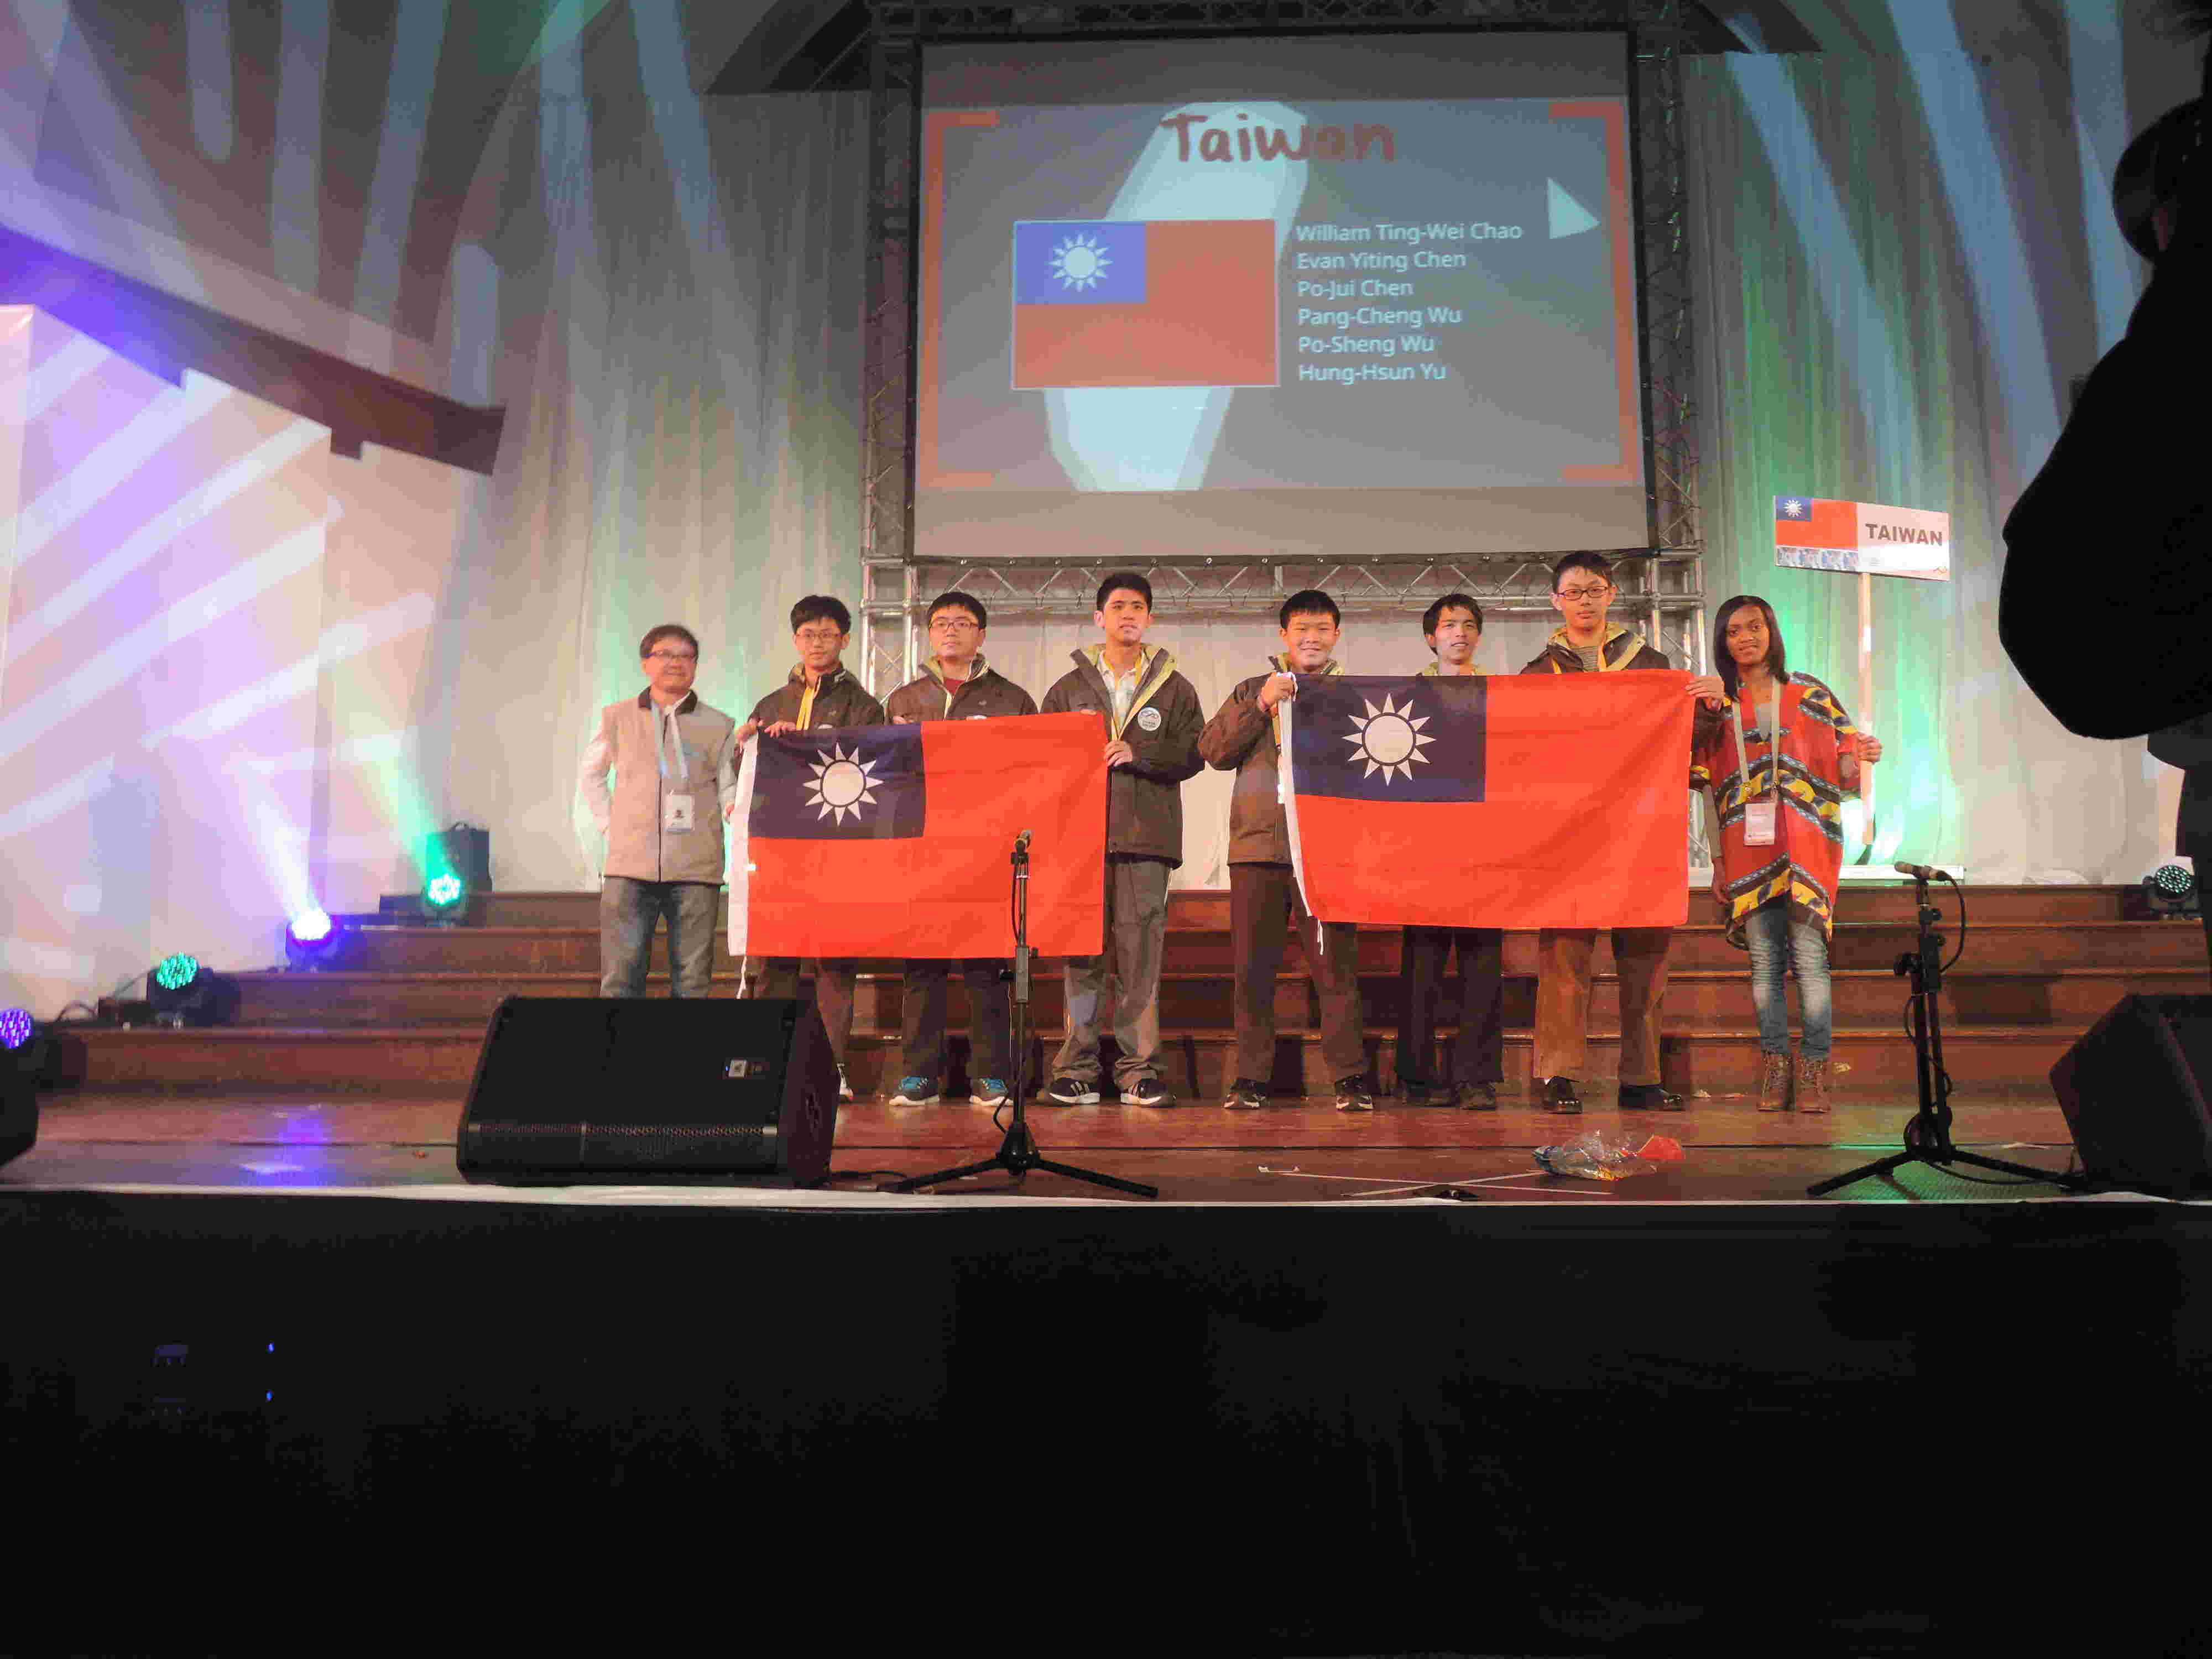
\includegraphics[width=0.5\textwidth]{media/opentaiwan.jpg}
  \caption{Taiwan at the opening ceremony.}
\end{figure}


After that we have the stage-walk for all the countries that joined after South Africa. We discover that the later a country joins,
the more difficulty CBD has figuring out what the Chinese translation for that country's name is.
% I'll leave the reader to guess why this might be the case.
We then have a performance from some (literal) clowns,
including a rather hilarious scene where two contestants (volunteers) of opposite genders
are selected to go on the stage and placed in rather awkward situations. I feel sorry for the volunteers.

Finally, at the end of the opening ceremony the organizers try to take a ``group picture'' in the auditorium from the balcony. Considering the number
of contestants, this goes about as well as you might think it would. By the time the ceremony ends, it is 7:30 PM, rather than the scheduled
7PM. Unfortunately, this is not good news in terms of dinner, which only lasts from 7PM to 9PM. Everyone rushes back, but as usual the buses
are too few in number and most people end up waiting for the next bus to come.
The Taiwan decides to just forgo the bus and take the 15-minute walk back to the dorms. Needless to stay, roughly thirty seconds after we
step out of line for the bus, another two completely empty buses arrive.

By the time we get back at 8PM the dining hall is intolerably crowded. The line moves quickly enough, but with everyone coming in at
once the hall quickly run out of seats. About four or five teams form a circle on the ground of the east half to eat their meal while the
nearby Canada team simply eats standing. The Taiwan team stands in the west half, and fortunately about 10 minutes in the Ecuador team
generously gives us their table as they are about to leave.

Posting dinner we finally obtain Wi-Fi credentials which have been posted in the deputy leader's dorm as well as our own.
It is now almost 9PM, and everyone is exhausted, so this time the entire team decides to not shower. We also decide that taking a shower
is far too cold and agree to simply not shower until after the test, lest we fall ill just in time for the contest.
Thus everyone retires to sleep.

\section{July 8 -- IMO Day 1}
After an early breakfast we are shipped on the ever-inefficient buses
to the examination room.
I make the wise decision to stand near the staircase meaning we and the Canadians are the first to enter.
The room consists of six blocks, three blocks in each hall.

\begin{figure}[ht]
  \centering
  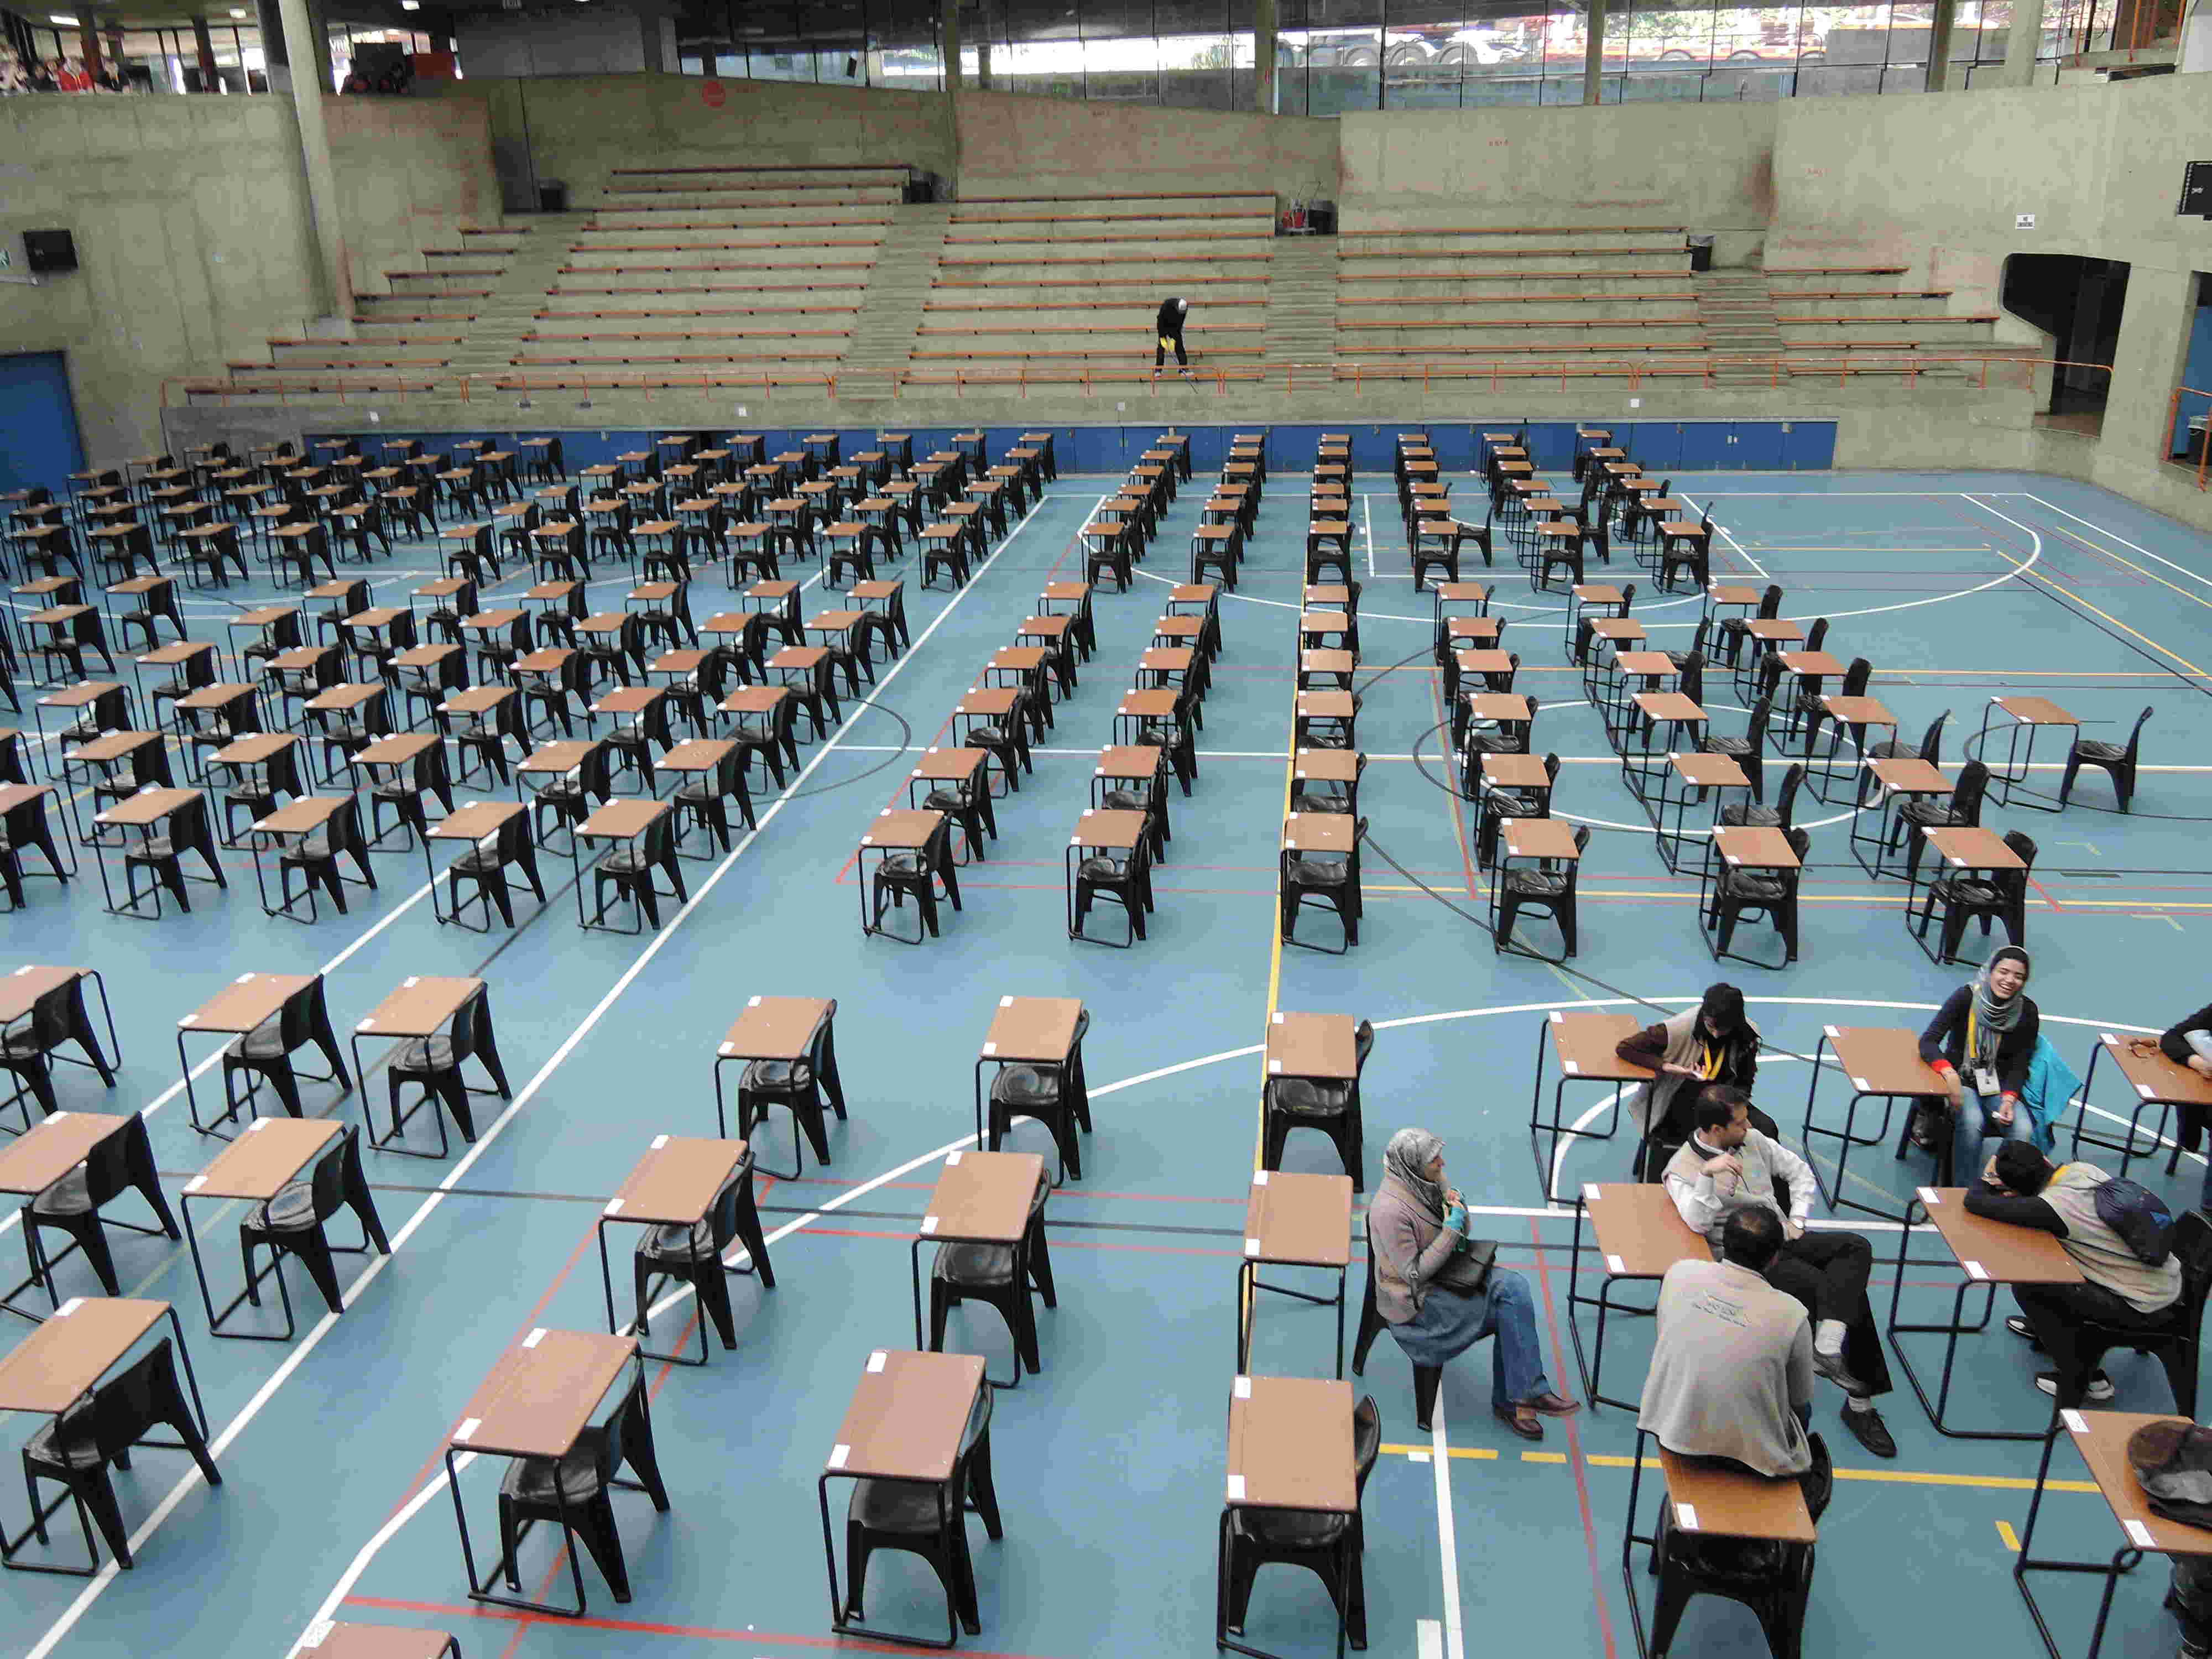
\includegraphics[width=0.5\textwidth]{media/contest_venue.jpg}
  \caption{Testing room.}
\end{figure}

Amusingly, they decide to place curtains between the two halls, leading me to joke that ``now we can only cheat off half the people''.
Per the code TWN2, I am placed in Block 2. The instructions claim that the back of our name tags specify where in the block we should be, but this is false; the back of our name tags are blank.

We were told to bring our contest materials in a provided transparent plastic bag. Unfortunately, said bag is not actually large enough to fit a compass, ruler, or a jacket, so I have to hand-carry a lot of things.

Anyways, the contest itself proceeds smoothly logistically.
We start abruptly (i.e.\ with no warning) a few minutes before 9AM,
with a strange rule that we made read the problems but not write anything until 9AM.
The contest folder contains a copy of the problems, a folder to place the answer sheets for each problem, ten blank answer sheets, and a series of cards used to call the attention of the invigilators:
\begin{itemize}
  \ii The white card is used to request an additional five sheets of paper.
  \ii The blue card is used to request a bottle of water.
  \ii The green card is used to request a bathroom trip.
  \ii The orange card is used for sending questions to the jury.
  \ii The red card is used to leave early and/or get other help.
\end{itemize}
Despite feeling cold before the test, I immediately shed my jacket once the test begins.

Overall things run pretty smoothly. We start and end on time and nothing appears to go wrong, which I consider a small miracle knowing first-hand that something always goes wrong.
I solve all three problems.
Details of the actual contest sitting are in the contest analysis.

After the test I discover that three other contestants on the Taiwan team have aced the first day. The remaining have solved IMO1 and IMO2. The consensus seems to be that IMO1 and IMO2 were quite easy this year and IMO3 was a medium-hard problem.
The USA team has gotten trolled by IMO3, claiming only two complete solutions and a potential 5+ partial.

During discussions at lunch it seems that the Taiwan score today is very high relative to many of the other strong teams.
Later we speculated that China probably aced the first day completely.
We would also later hear that Japan and Vietnam perform about the same as USA.

We return after Day 1 to the dorms, and as usual get on our laptops and start typing random things.
Pang-Cheng takes the time to try and verify some conjectures on GeoGebra
that he submitted for problem 3; it turns out they were both correct.
I take the time to check out the game room, where I meet the Isarel and Hungary team and join them in a game of Coup,
a surprisingly fun game of deception and politics.

When I return to the central room 406, I find that CBD has gone to sleep and Ting-Wei is somewhere else.
A couple moments later Ting-Wei comes complaining of a severe headache.
By ``severe'' I mean he is moaning in pain and I'm afraid that it won't go away.
Our efforts to call our deputy leader fail.
As a result I travel to Baxter directly in search of them, but end up
bothering one of the Observer B's in an adjacent room.
At the very least, I obtain the room number of Dr.\ Hong in case anything
else happens in the future.

On the way there I notice the room outside Baxter has a piano
which one of the Canadian contestants is playing 童話, which breaks
my heart as I had heard this from the Chinese Singing Troupe.
Later when I find a chance I return to play on the piano, to discover that
the keys are incredibly light, making it suitable for my Chopin and Ravel
but not for my Guilty Crown.
On the way back I see several teams playing soccer on the field outside.
I wonder where most of the other teams are.

When I get back Ting-Wei is feeling infinitely better, insisting that all
it took was to dress slightly warmer.
We proceed on the way to dinner, except CBD accidentally locks himself out of his room and we are forced to get the master key.
The guy in the lobby  uses Google Translate to tell us there is a R30 fine (roughly 3USD)
for this. Dr.\ Hung later reports that he did not have a similar fine.

In light of the crowding, our meal venue has been changed to Baxter.
We grab dinner and hilariously run into a table which has the board
to problem 2 set up using butter and silverware.

\begin{figure}[ht]
  \centering
  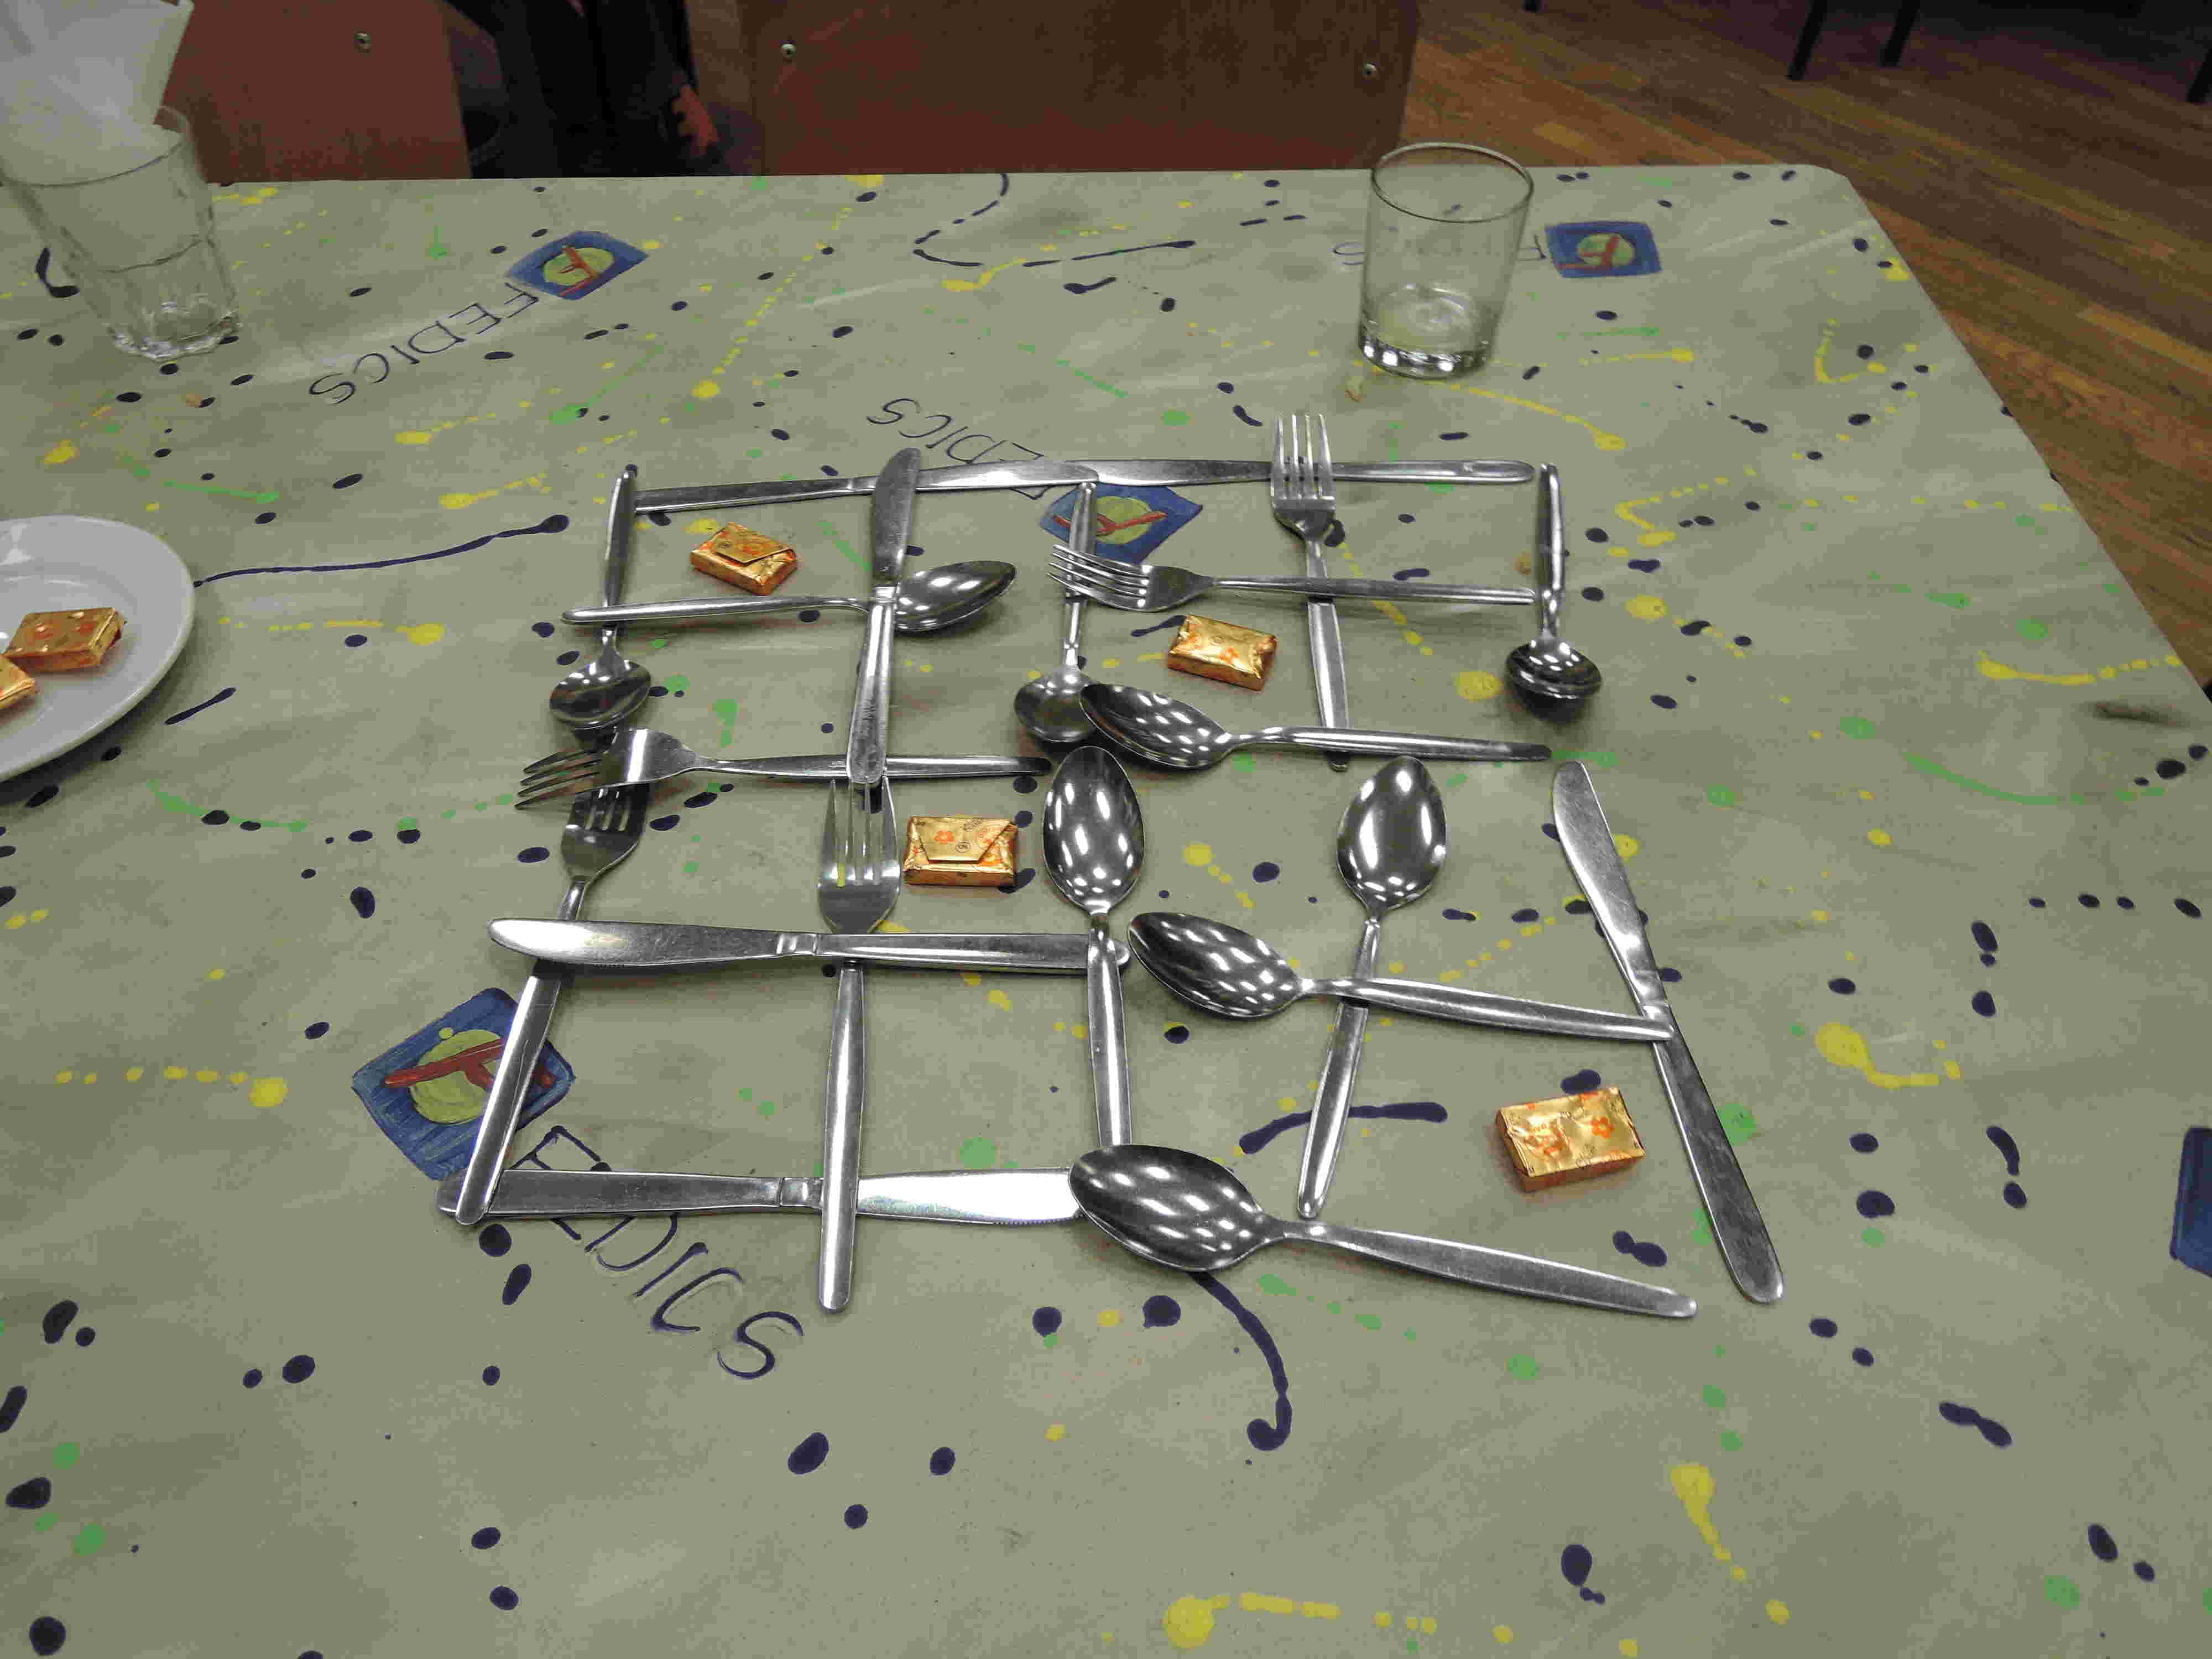
\includegraphics[width=0.5\textwidth]{media/epicwin.jpg}
  \caption{Someone solves Problem 2 for $n=4$.}
\end{figure}


Finally it is late and we head back to 406. I type at my report while the others play Mao.
CBD and I then go online searching for the Black Bullet theme, to little avail as the Internet in 406 is quite shady.
I'm not sure why; my room 402 seems much more reliable in terms of connectivity.

I end up sleeping too late, at around 10PM.

\section{July 9 -- IMO Day 2}
We begin the morning by singing modified versions of the alphabet song, and agree that any song should contain
the words ``CBD'' and ``轉眼匹''.

At breakfast the person standing guard at the door becomes very confused, because she has evidently not informed
that certain teams were moved to Baxter and insists we should be at Leo. Nonetheless we manage to get through after
some minutes of negotiation.

Then, the actual IMO takes place.

\begin{figure}[ht]
  \centering
  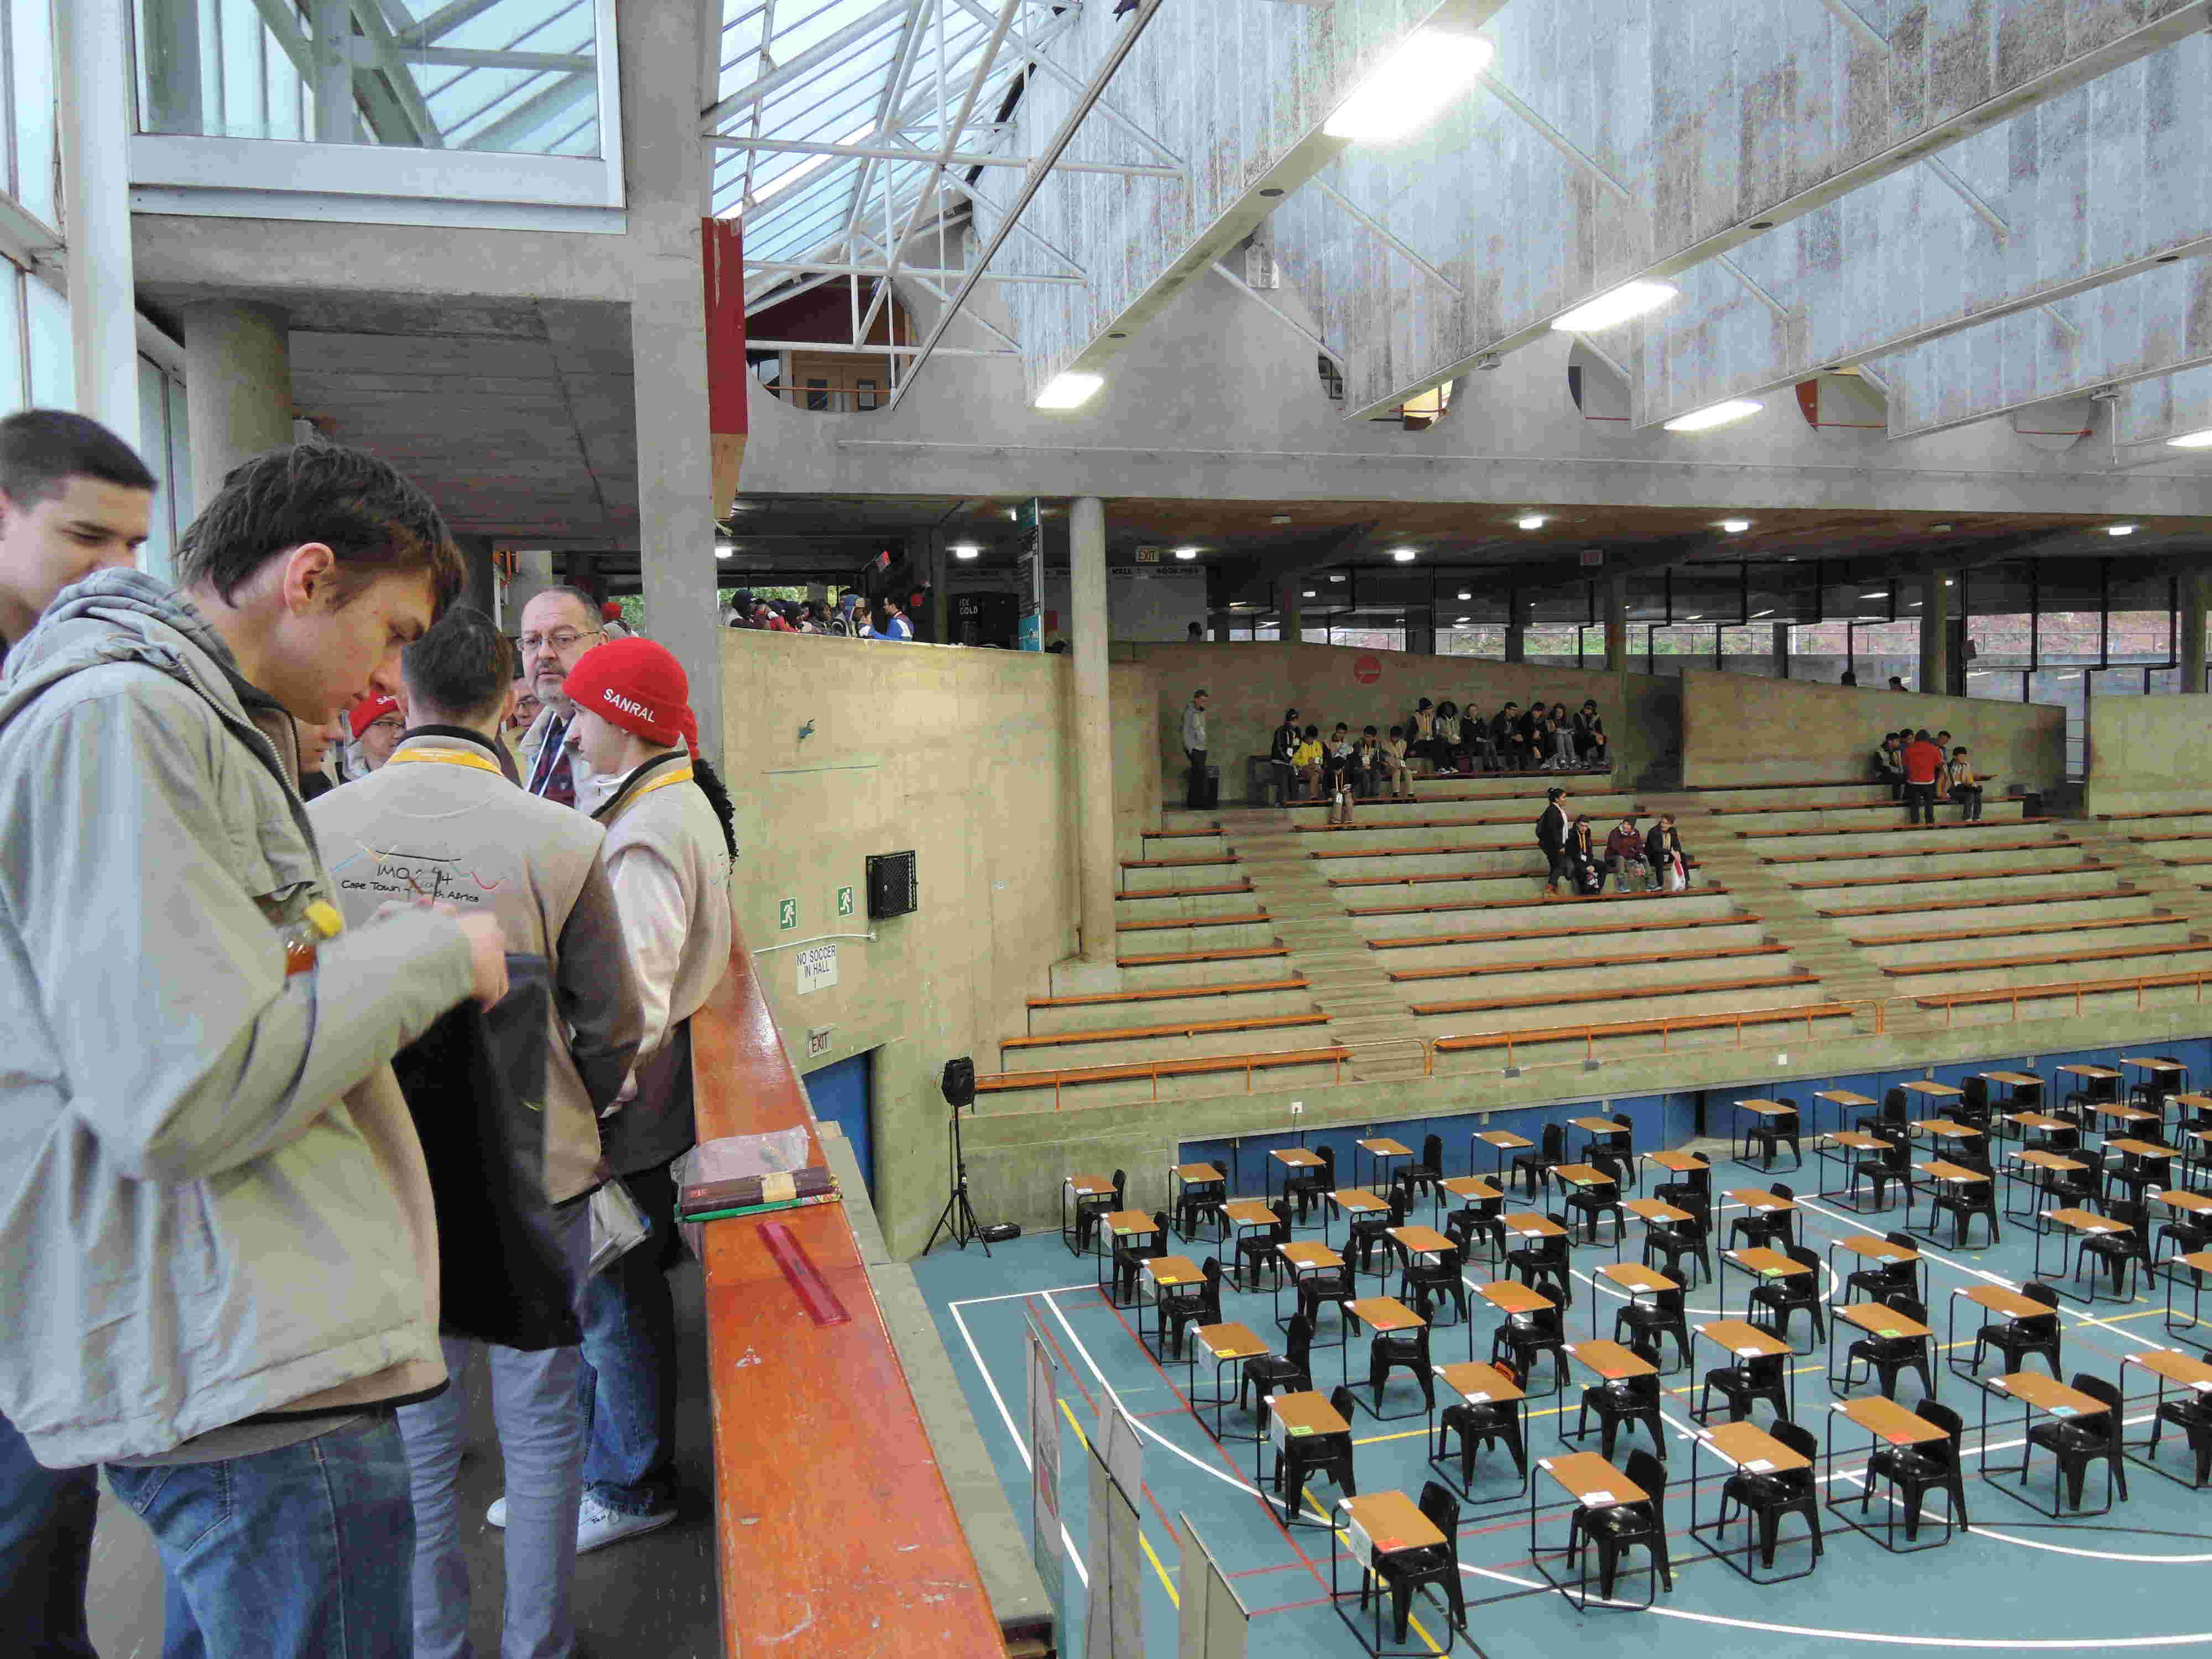
\includegraphics[width=0.5\textwidth]{media/IMO_D2.jpg}
  \caption{Just before Day 2.}
\end{figure}

Once again the invigilators run the contest smoothly.
The contest itself has a weird point -- the note in problem 6 specifies that proving the bound for other values of $c$
merits partial credit. I ask to clarify the maximum points obtained for proving a weaker value for $c$, but inadvertently
I have misread the question as $\sqrt n / c$ instead of $c \sqrt n$. Consequently my query of $c > 1$ leads the jury
to some confusion, and the reply is merely ``7''. The jury is a troll.

I leave the contest with two problems solved, and in somewhat of a state of despair at having
had to face two combinatorics problems on the same day.
(In USAMO 2013, Day 1 was also GCC, and my poor performance on that day had cost me USA IMO slots for both 2013 and 2014.)

After the contest and lunch I visit the games room to see if anything of interest is happening.
I sit down for a game of chess with UGA3, playing as black.
The game takes a while, but I effectively win once I manage to trap
his rook. To my left several people are playing Mao for the first time.
It is quite a spectacle.

I return to find that I have failed to lock my door upon leaving. Fortunately, nothing appears to
have been taken. I muse that the lock system is quite antiquated.
I join the others for Big Two in Room 406, being dealt rather unfortunate hands, though
I do win once going off a straight to 6.

At around 4PM we meet with our team leader again to prepare for coordination.
Problems two, four, six will be coordinated tomorrow in that order, followed by problems five, three, and one.
Evidently the rubric for \#1 used to specify deducting one point for not proving that a strictly increasing
integer sequence is unbounded (namely, you must mention ``integers''), but it appears this was removed
from the rubric, thankfully for me.
Some other contestants may lose a point for not explicitly checking $a_0 < a_0 + a_1$ as the $n=1$ base case.
Our team leader confides to us that in fact \#5 was ``N'', much to my dismay.
We also hear that China only has three solves on yesterday's geometry.

We discuss what we have done on the problems briefly with our leader, who then sends us back to our
rooms and asks us to write up solution sketches to \#2, \#3, \#5, and \#6, in preparation for coordination tomorrow.
I opt to type up the solutions as this takes considerably less time and gives more detail.
The result is Chapter~\ref{ch:solnsketch}.

We reconvene at dinner and discuss coordination further.
I am applauded for the pictures I submitted at Day 1.
Roger Lin also mentions standing in line with the two idiot questions that Ting-Wei and I
had submitted to the jury. Ting-Wei was trolling, I made an honest mistake, as I noted earlier.
I hope the jury was amused.

Sen-Peng Eu also mentions that the ``smiles'' that Ting-Wei had seen earlier were ``bitter smiles'' (苦笑) of despair.
% He also yells at Ting-Wei for having apparently shouted ``how do you solve C7'' as the leaders passed by -- this
% was intended to be last year's C7, but this obviously would have looked very bad if this year's C7 was on the IMO.

After dinner we return and I try to type up my diary of events, but am shortly interrupted to go to the ``war room''
and discuss my solution to \#6. My case does not take very long, it is merely briefly outlining the solution again,
and mentioning that while my typo of $\sqrt n / c$ in lieu of $c \sqrt n$ should hopefully not lose a point, it
may result in my $2$ becoming a $1$. I will be quite sad if that happens.
My leaders assure me they will fight for this second point if necessary, which they think I deserve (as do I).

During this time I also get to see the rubric for \#6, which specifies that
\begin{itemize}
  \ii Proving $\sqrt[3]{n}$ (hence $c=0$) is worth $1 - \eps$
  \ii Proving any $c > 0$ is worth $2 - \eps$.
  \ii Proving $c = 2^{-\half}$ is worth $3 - \eps$
  \ii Proving $2^{-\half} < c < 1$ is worth $4 - \eps$, and
  \ii Proving $c=1$ is of course worth the usual $7 - \eps$.
\end{itemize}

On the way back I run into the USA team, modulo Josh Brakensiek.
We discuss about the IMO and a lot of things in general, including a ``robust'' problem.
\begin{problem*}[China TST 2006]
  For a positive integer $M$, if there exist integers $a$, $b$, $c$ and $d$ so that:
  \[ M \leq a \leq b < c \leq d \leq M+49, \qquad ad=bc \]
  then we call $M$ a GOOD number, if not then $M$ is BAD. Please find the greatest GOOD number and the smallest BAD number.
\end{problem*}
Solution: bash.

During this time I run into AUS1 Alex Gunning, who claims to have solved all six problems.
This is the first six-problem claim I've heard other than TWN5 Po-Sheng Wu. Surprisingly, I find myself quite happy for him.
It is a great feeling to solve all six problems at the IMO and Alex is all smiles.

The USA team heads up to the 10th floor of Leo, where Canada is apparently housed.
We invade Alex Whatley's room, and Sammy tries to fly some games of Mafia.
The first one ends in Jester getting lynched (nice job Yang).
In the second game, Cupid pairs Kevin Sun and Mark Sellke, because of course they would get paired.
Kevin turns out to be Night Vigilante and Mark Sellke turns out to be Doctor.
The result is quite hilarious:
On the first night Mark heals himself when Kevin tries to vig (kill) him, and on the second night Mark heals Kevin when he tries to vig himself.

\begin{figure}[ht]
  \centering
  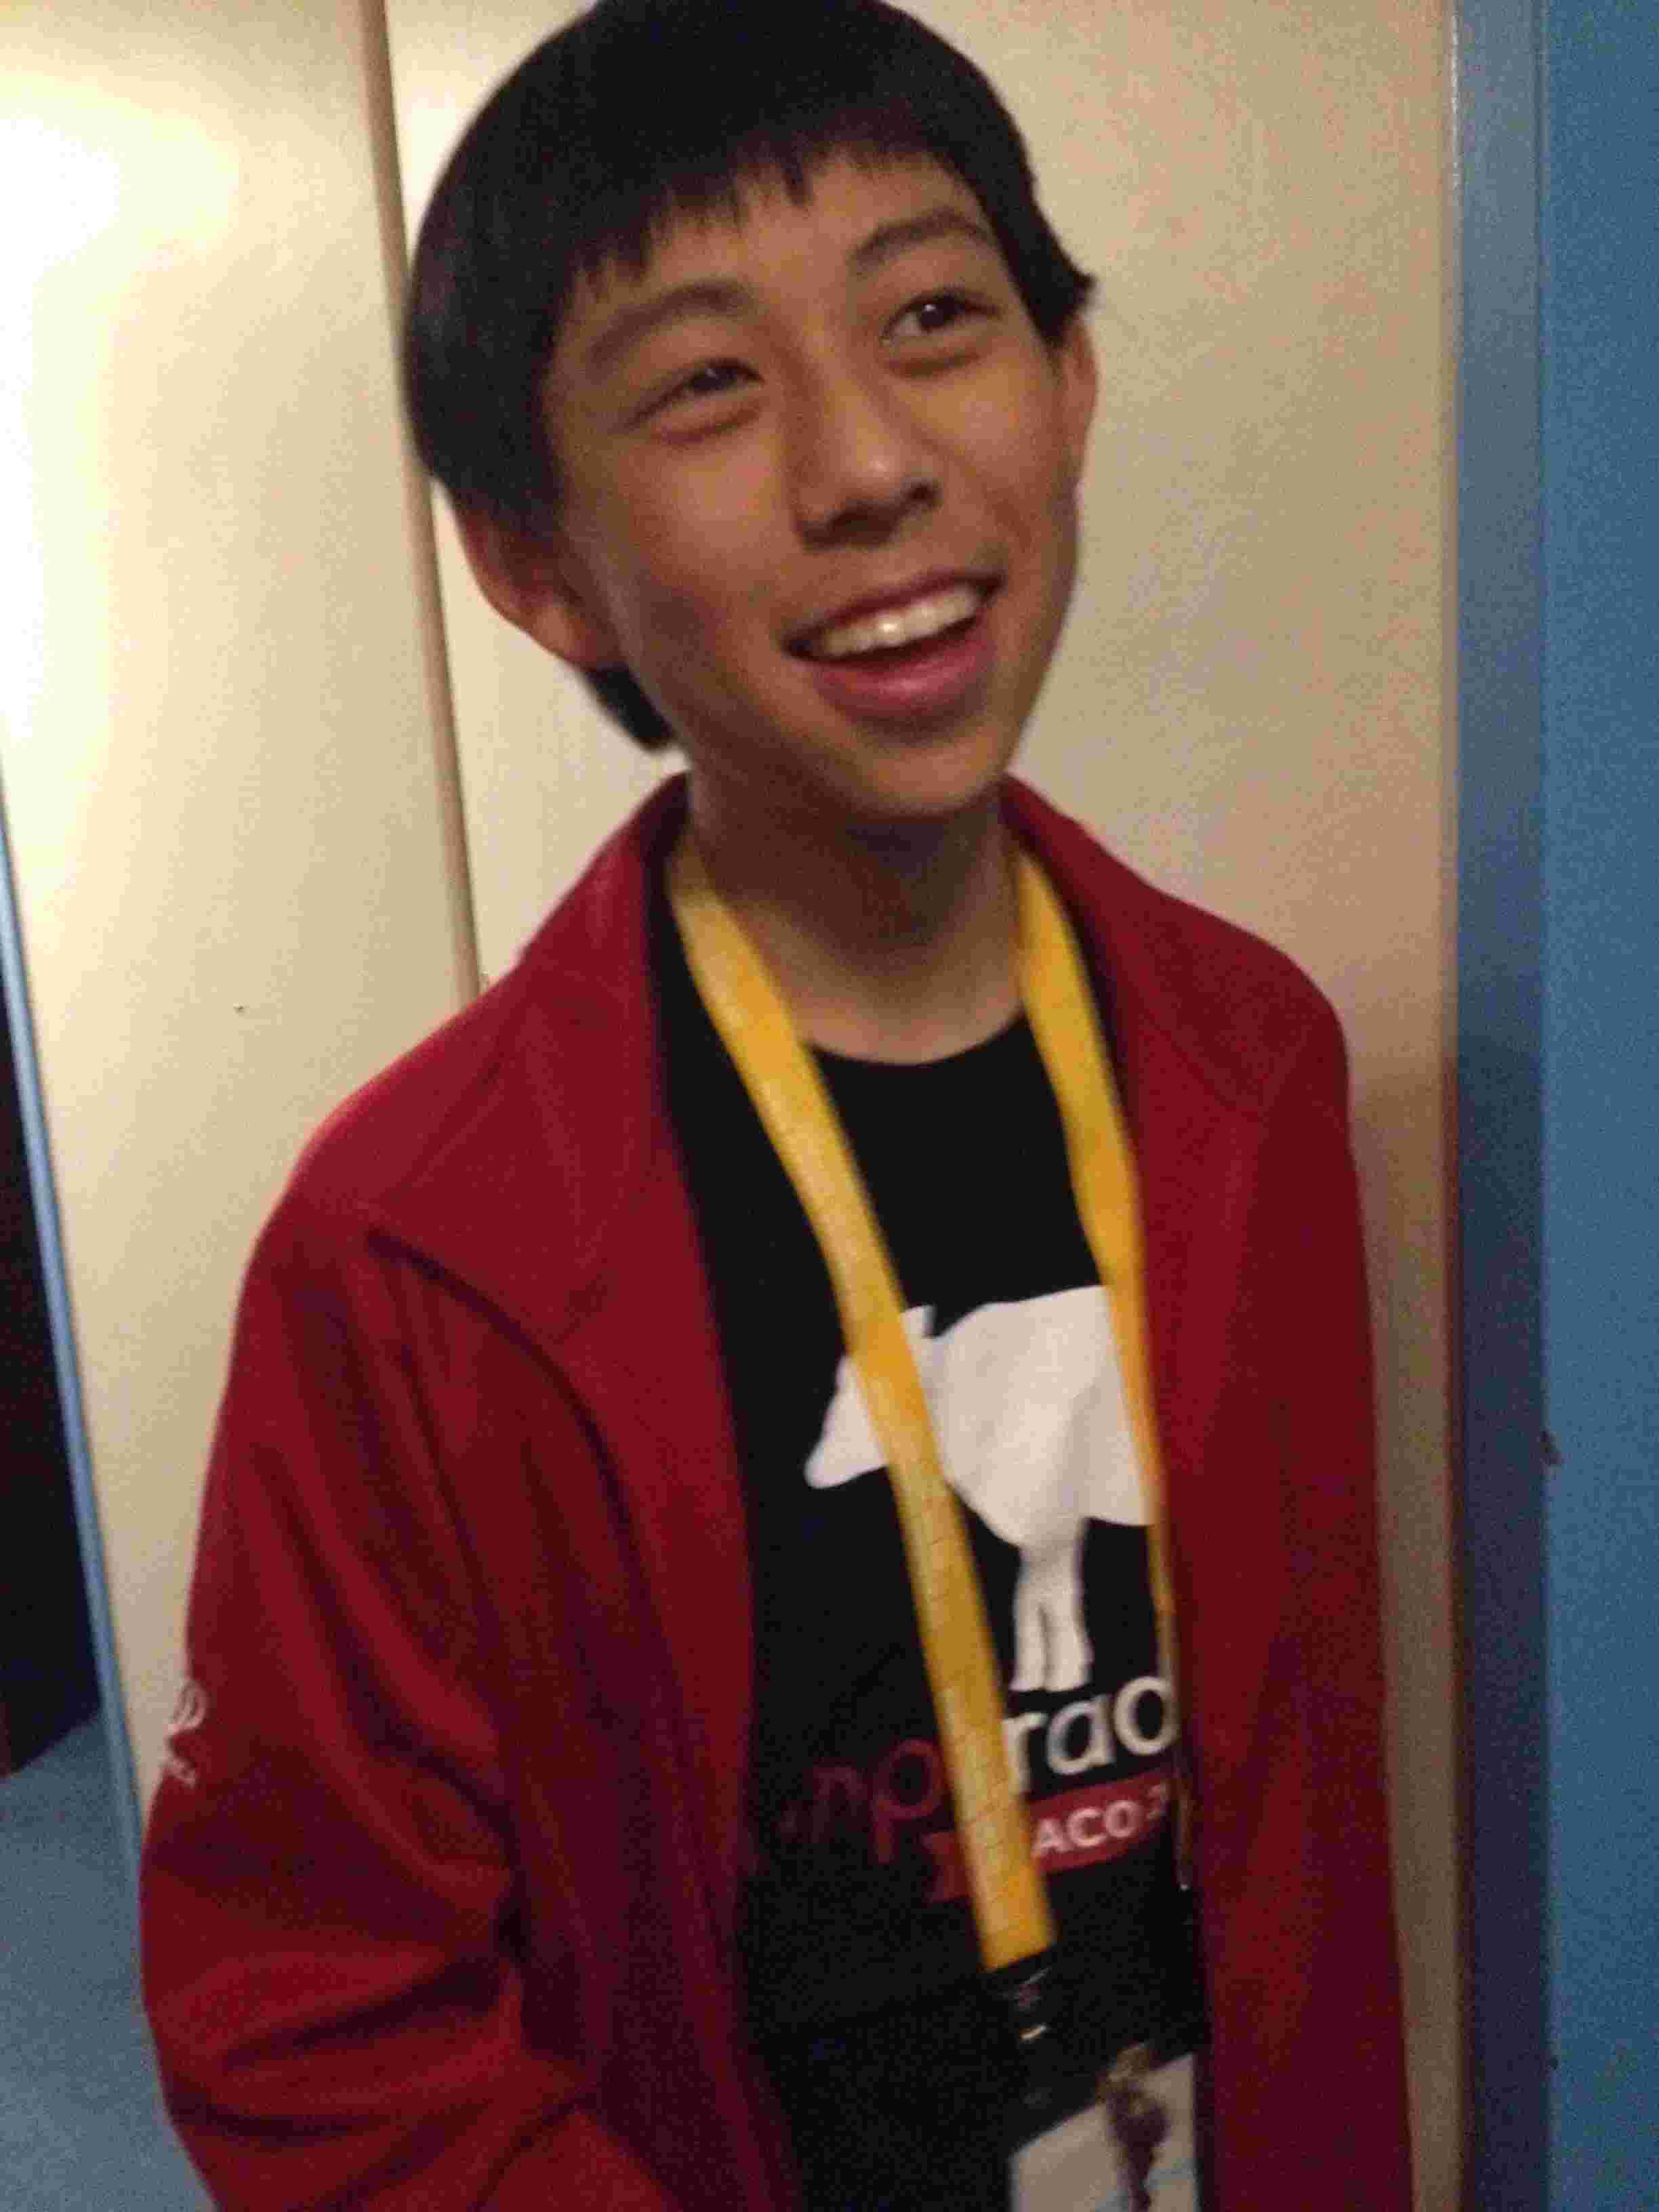
\includegraphics[width=4cm]{media/ksun.jpg}
  \caption{Kevin Sun.}
\end{figure}


Afterwards I retire for the night, preparing for the excursion tomorrow.
The Ukraine team passes by my room and for the first time I realize they are in fact our neighbors on the fourth floor.

\section{July 10 -- Excursion}
As I prepare to leave in the morning for excursion, I discover that my Taiwan IMO jacket is missing.
I must have lost it on the way back from IMO Day 2.
I am really good at this life thing\dots
I hope it turns up soon.
This leaves me in a sour mood for the rest of the morning.

While coordination happens today, the contestants are farmed into a large group of buses.
We are placed in Bus 10, with a tour guide Greg; a total of 42 people are placed on the bus.
Some things Greg mentions to us:
\begin{itemize}
  \ii Do not mention to any South Africans that they ``sound like an Australian''.
  \ii Traffic lights are known as ``robots''.
  \ii The South Africans drive on the left side of the street as a result of the British annexation.
  \ii Stay on this bus even though you might have friends or are attracted to someone on another bus.
\end{itemize}

We visit the Newlands and Chapman's Peak initially. I take pictures \emph{en masse} at all of the stops; the
scenery is truly gorgeous.
We also pass a long beach named Long Beach and a sunny valley named Sun Valley.
Greg mentions a large incidence of shark attacks on Long Beach.
We also pass through Table Mountain National Park, the home of a large number of African penguins.
Time passes very quickly while we observe them.
On the way back we again poke fun at a certain AG, translated as ``almost gold'', ``almost girl'',
``a girl'', and then ``absolutely girl''.

\begin{figure}[ht]
  \centering
  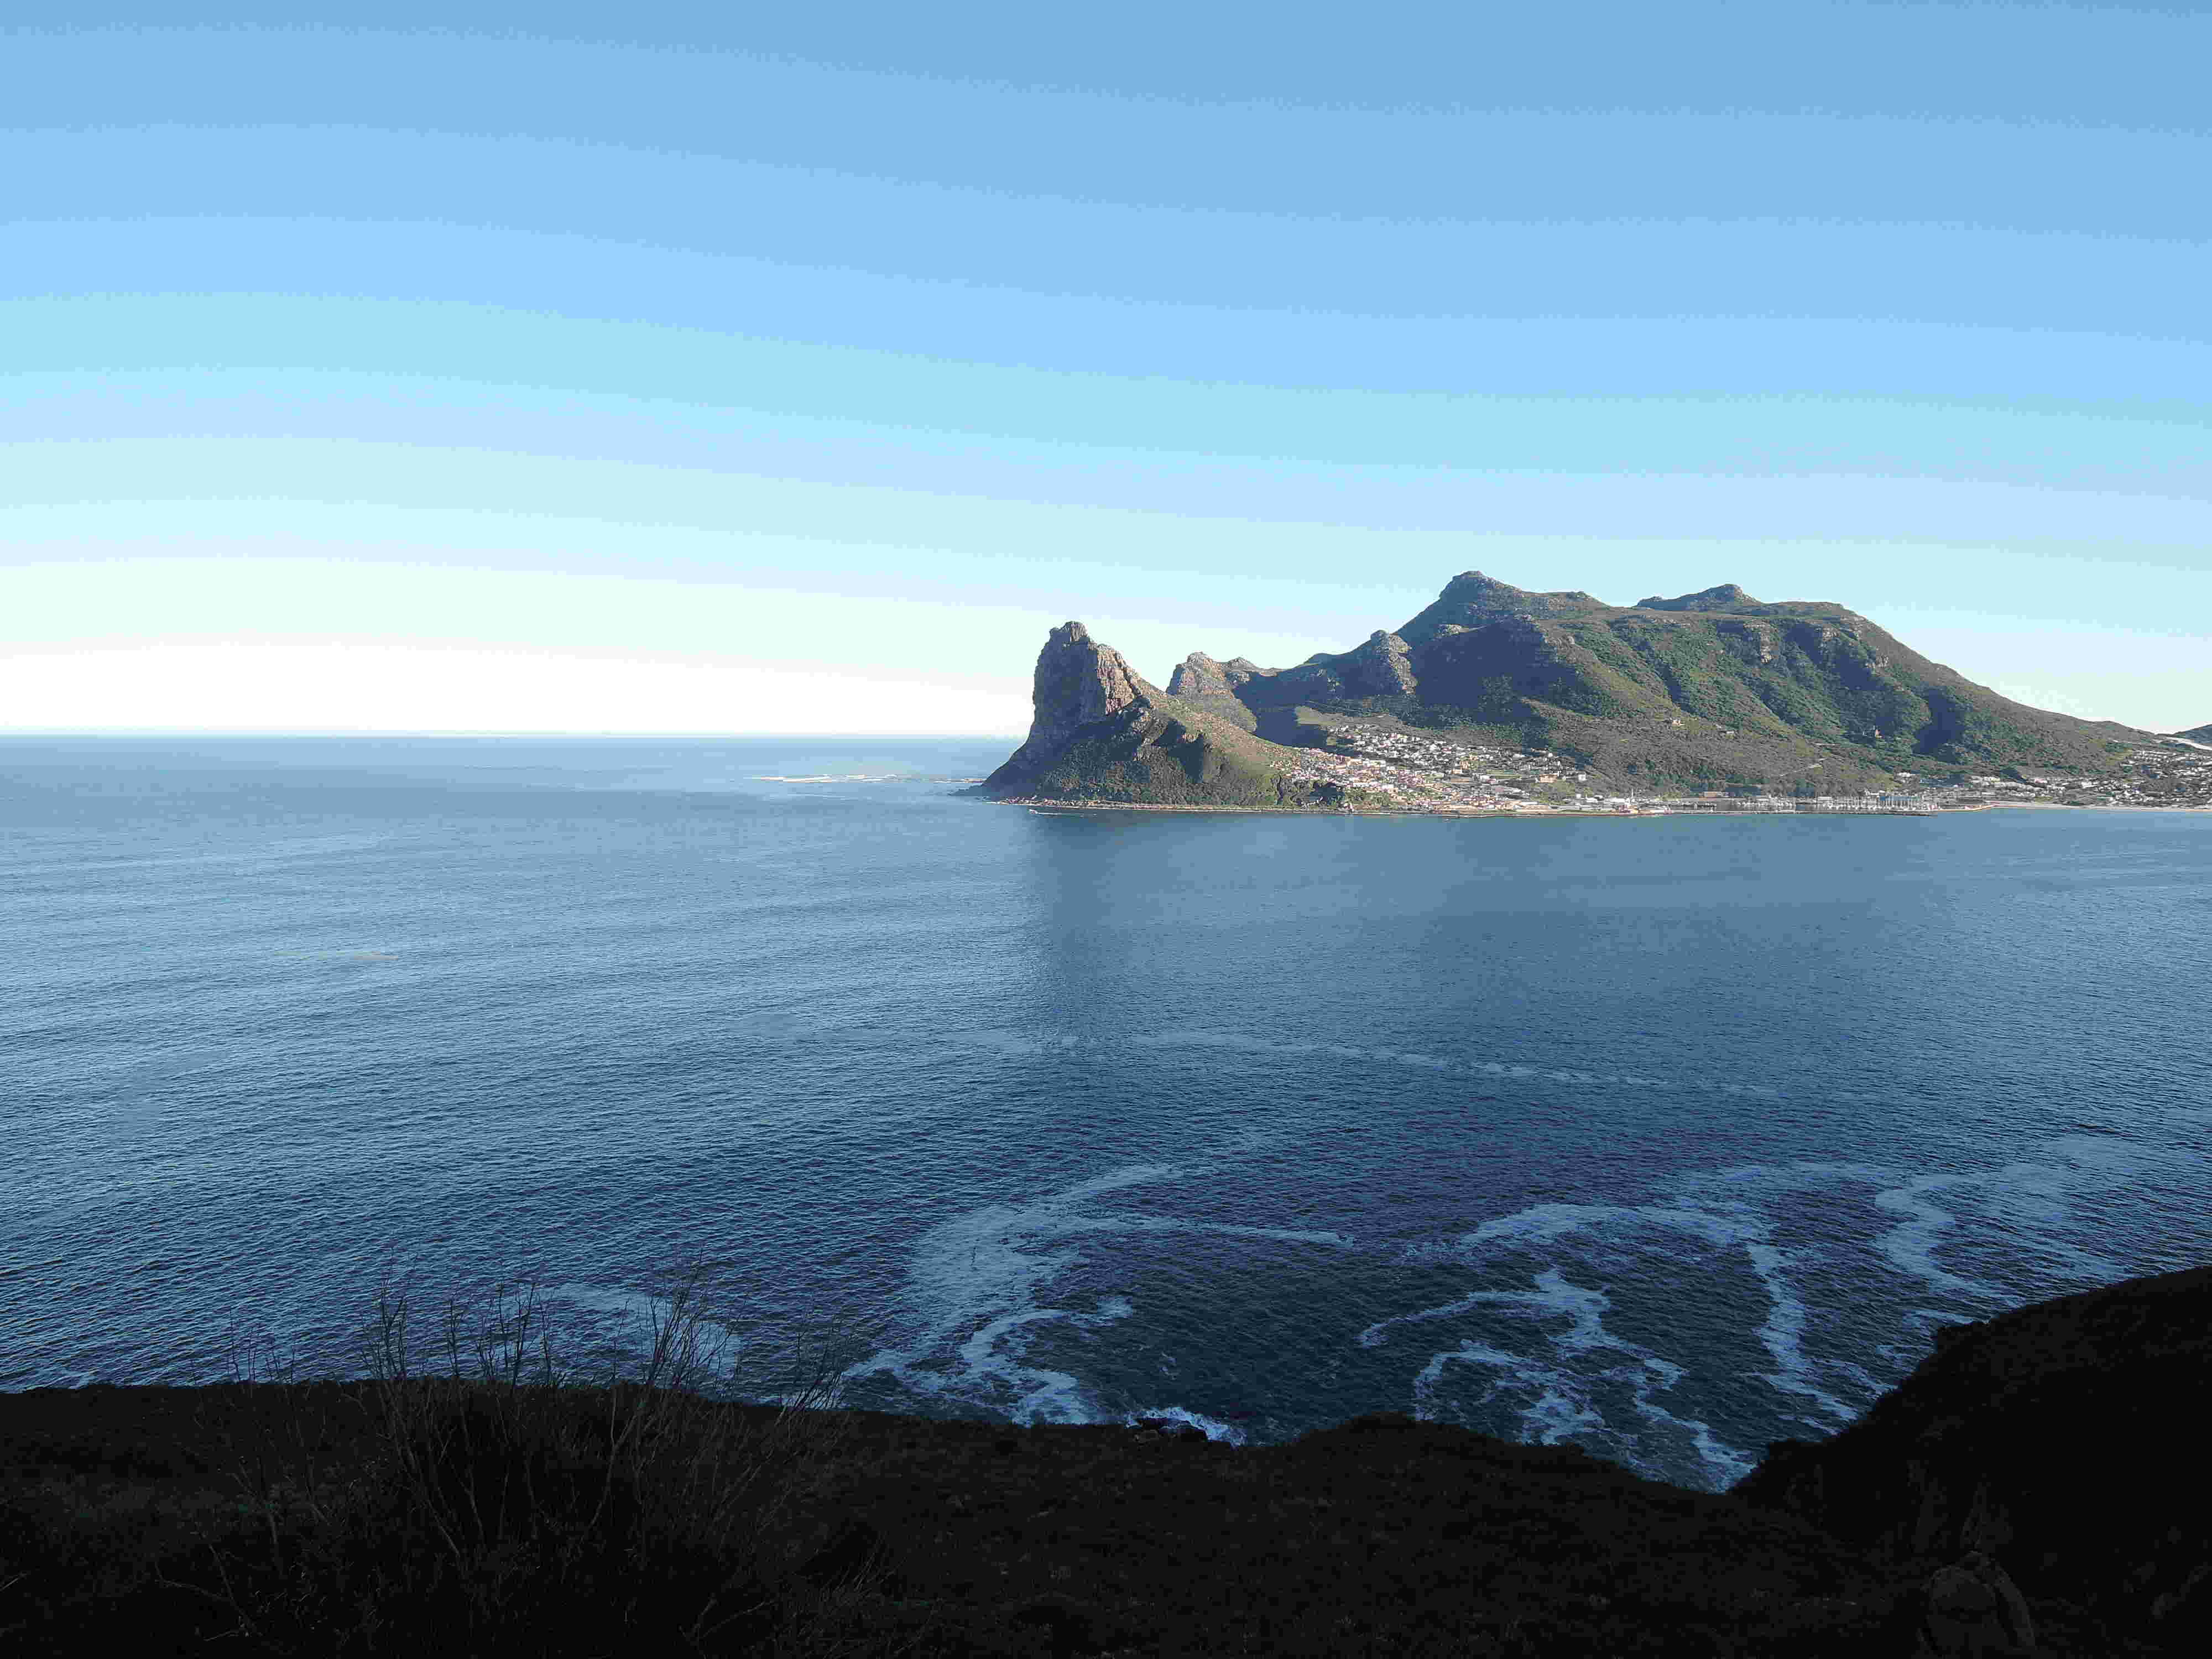
\includegraphics[width=0.5\textwidth]{media/scenery.jpg}
  \caption{Some views of the scenery.}
\end{figure}
\begin{figure}[ht]
  \centering
  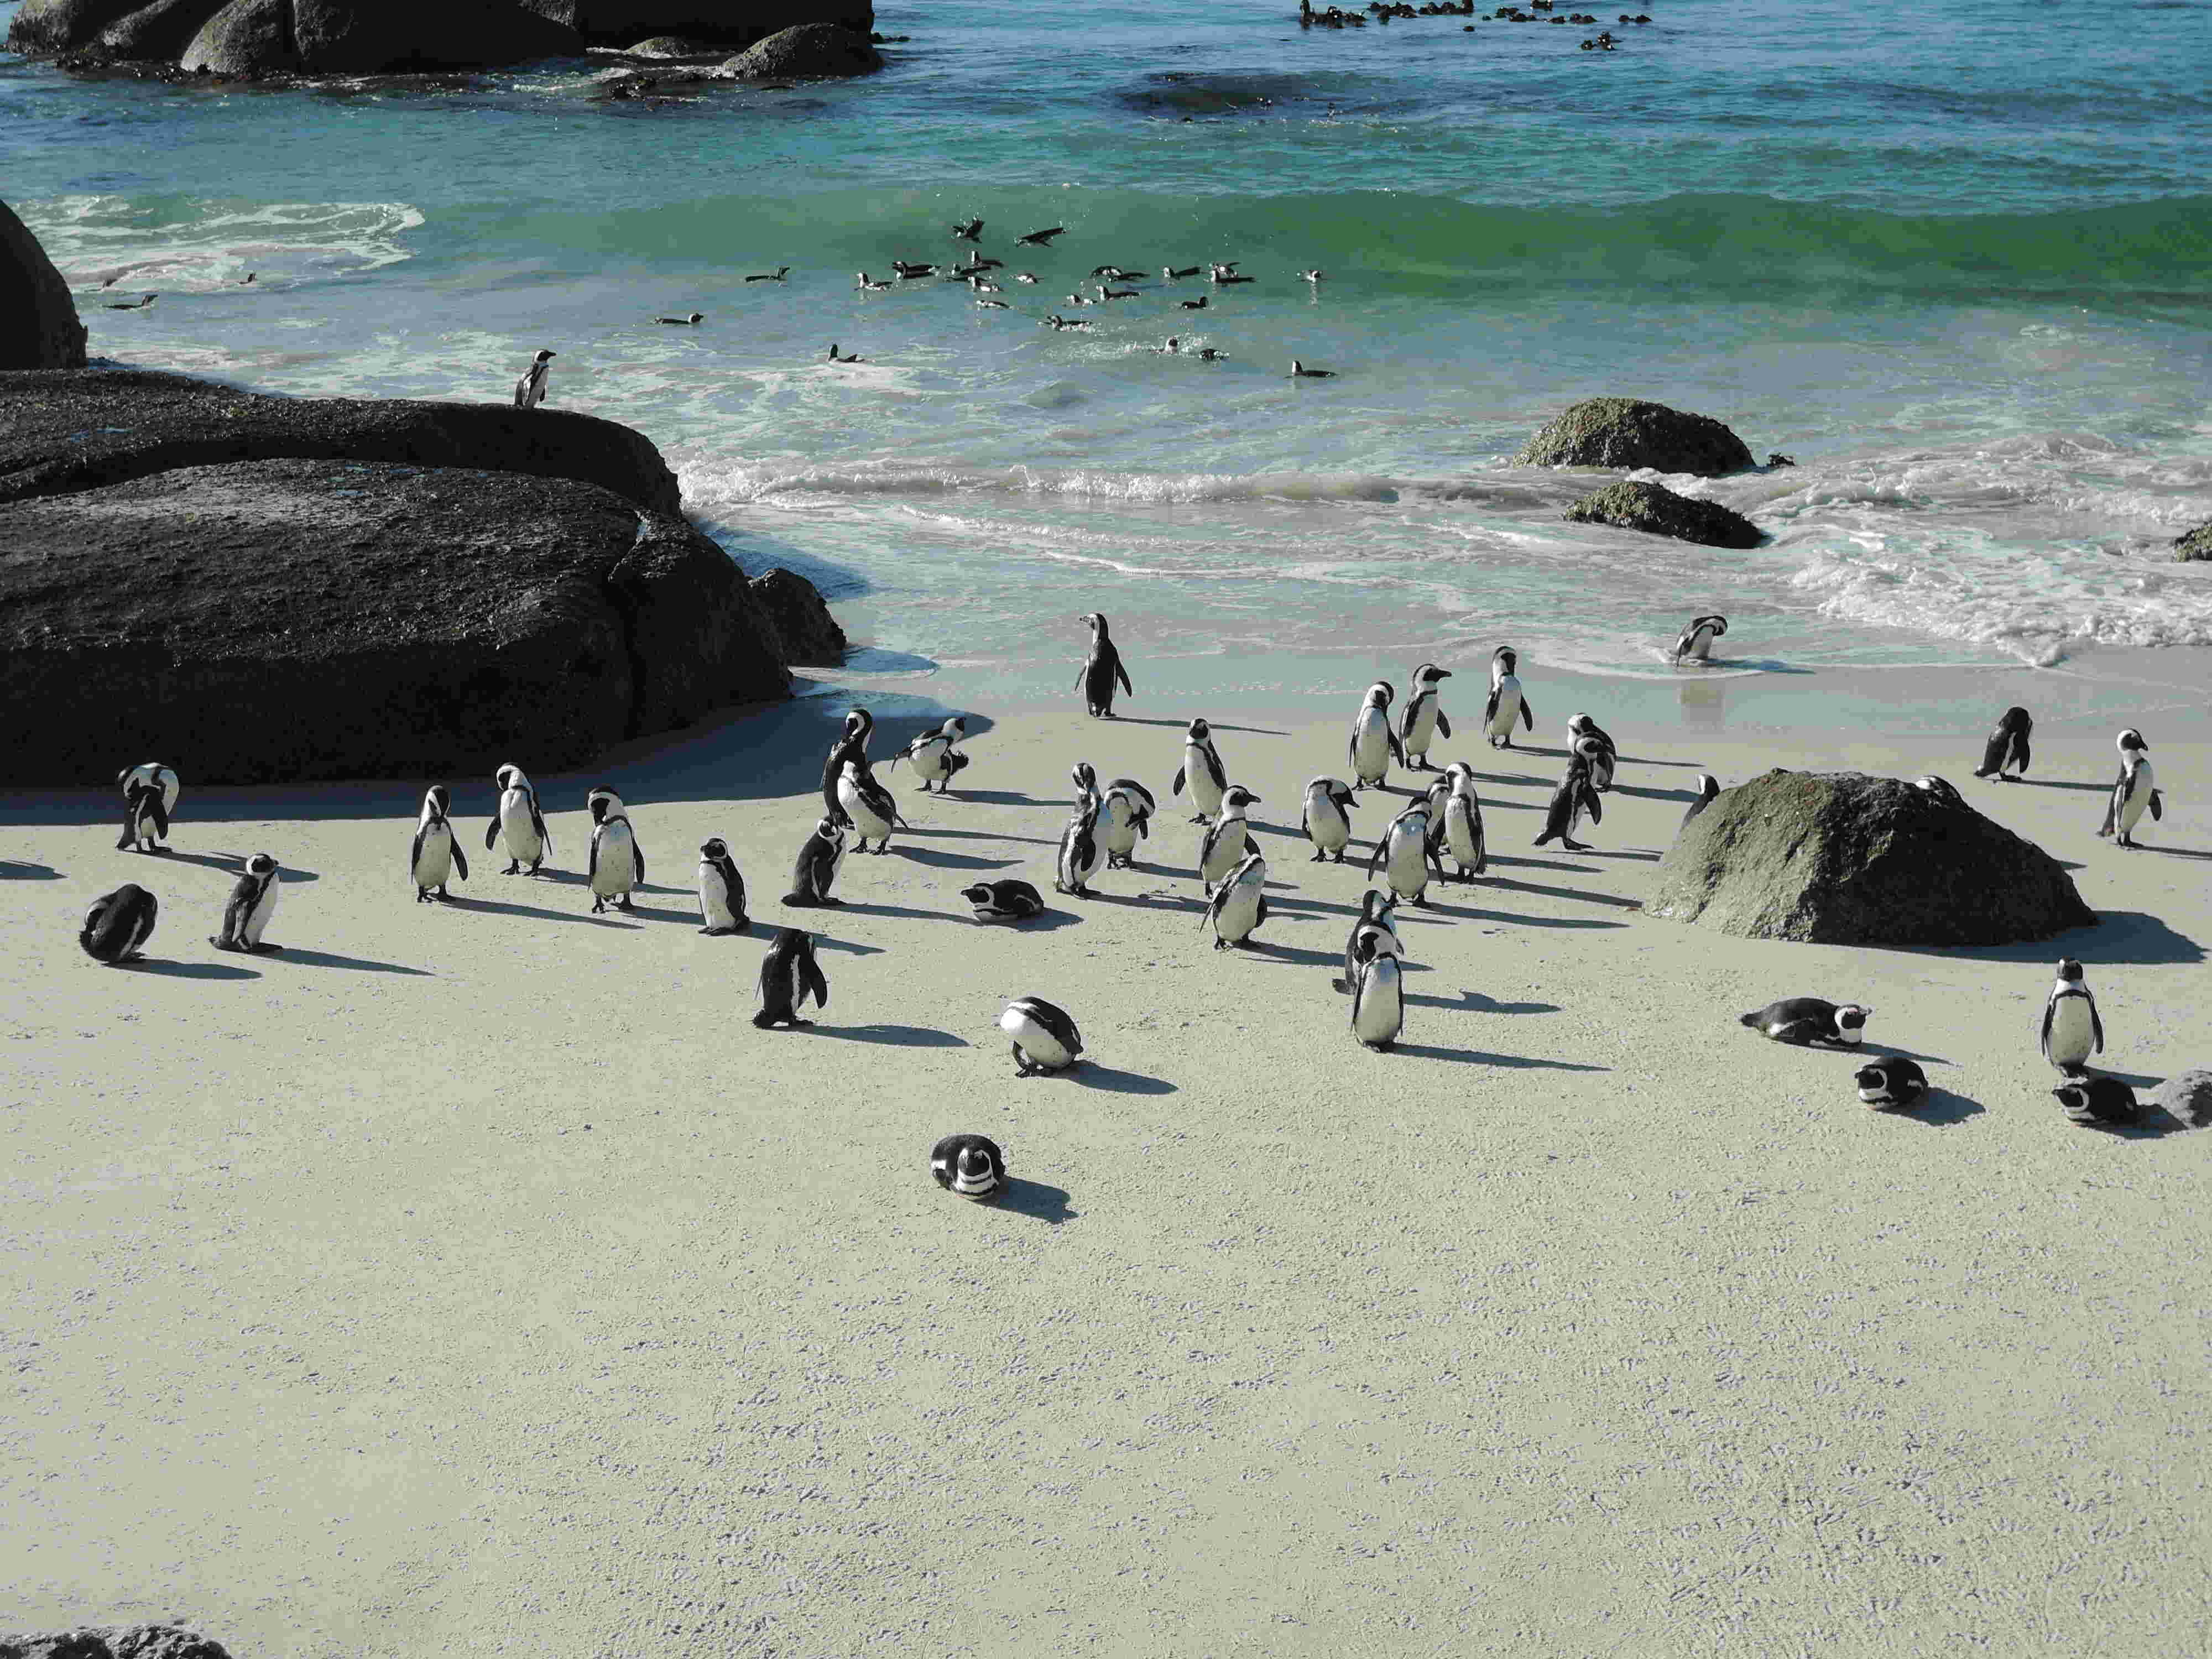
\includegraphics[width=0.5\textwidth]{media/penguins.jpg}
  \caption{African penguins.}
\end{figure}


For lunch we stop by a small location called Ocean View. It is the result of forced relocation during
the apartheid in South Africa some years ago. The lunch distribution is a logistical fiasco, having several
hundred contestants placed in a small room getting food more or less simultaneously.
The Ocean View organizers also present some entertainment in the form of songs and dances, some of which are
largely ignored. I do confess that I enjoyed the singing of ``Set Fire to the Rain'' and ``Because You Loved Me''.

I end up napping on the bus ride after lunch, but I think I wake up more tired than before.

Our next stop on the road is near Cape Point, which evidently is in fact not the meeting point of the two oceans.
We first stop for 10 minutes by a beach, where I continue taking pictures and laugh a couple of the
contestants try to skip rocks at the beach. Perhaps ``boulders'' is more accurate than ``rocks''.

We then take the bus towards the summit. Pang-Cheng plays Xiangqi on his phone, and I resolve to also download
the game on my tablet when I get home later.

Finally we arrive near the top of Cape Point. We are given about 50 minutes to enjoy the location.
The Taiwan team takes the climb to the very top, next to the lighthouse.
This climb is worth it -- the view is magnificent.
I take a moment to reflect just how far mathematical olympiads have taken me; it breaks my heart that
the journey will soon be over.

\begin{figure}[ht]
  \centering
  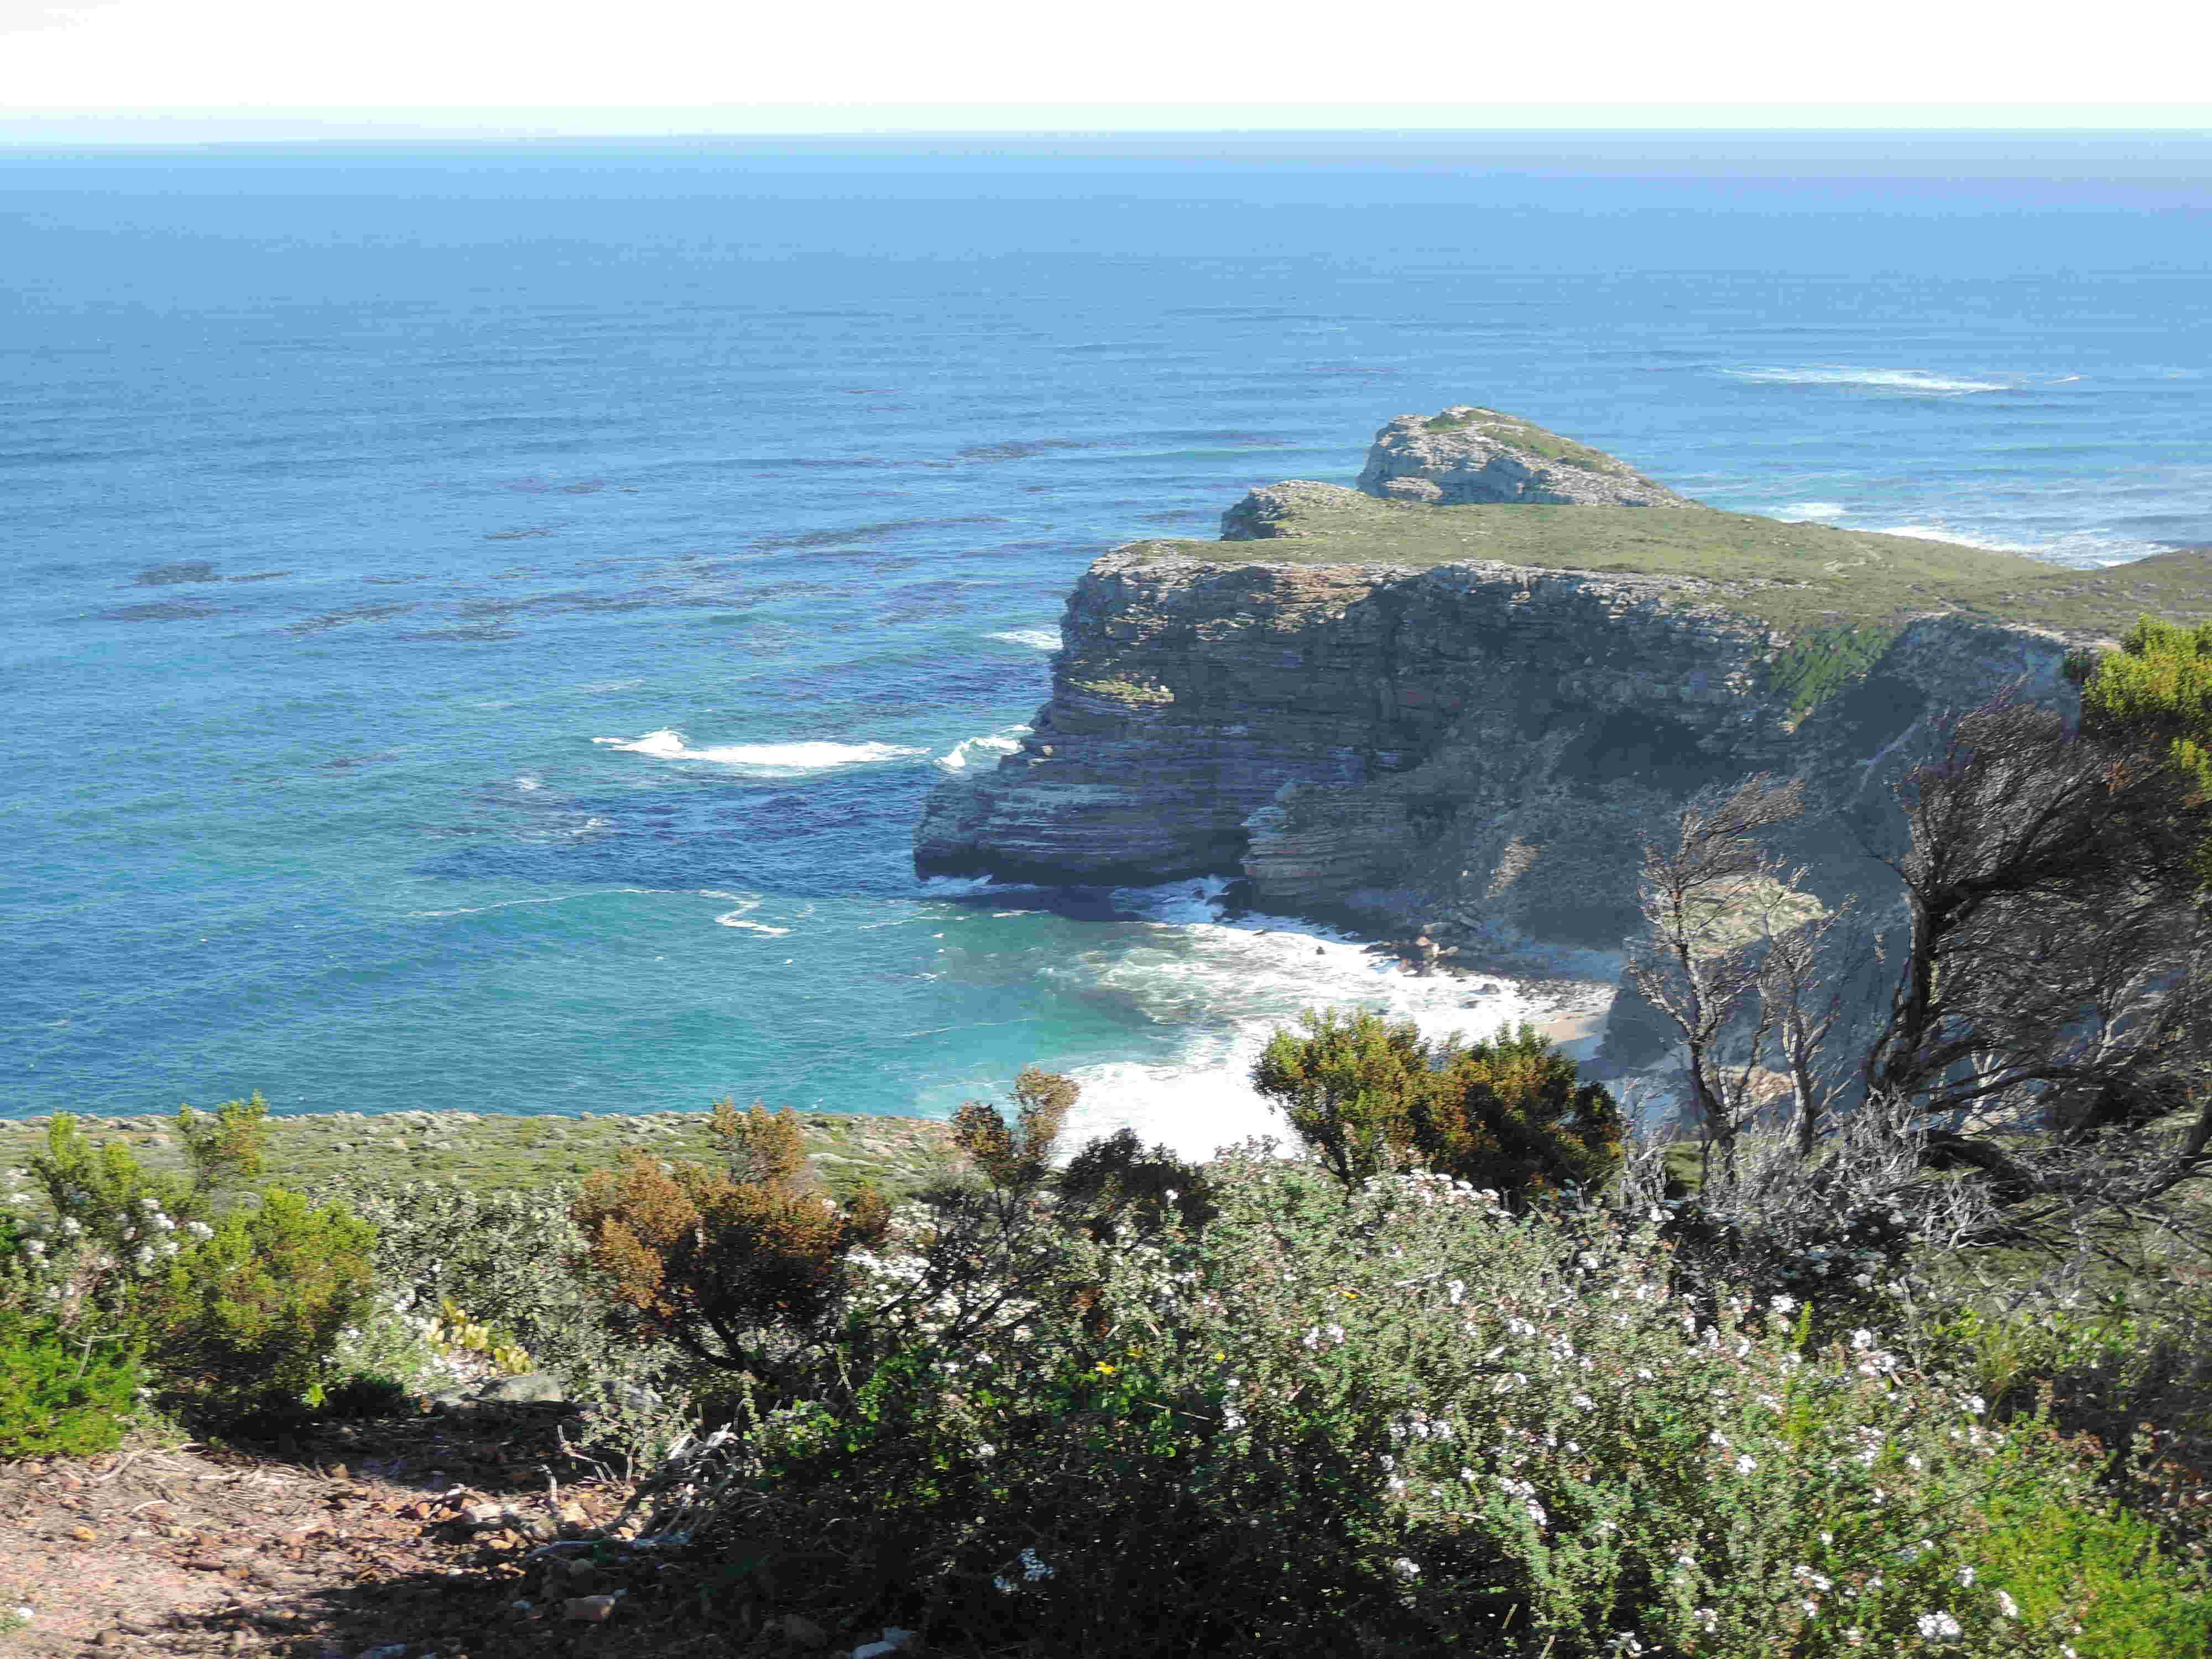
\includegraphics[width=0.5\textwidth]{media/lighthouse_tip.jpg}
  \caption{The view from the lighthouse.}
\end{figure}

At the lighthouse I notice that one of the contestants is wearing an MIT shirt.
After quickly asking I find that she is also going to Boston next fall.
All roads lead to MIT.

Ting-Wei buys a penguin from the gift store, saying that it is useful for poking CBD.
We then embark on the 90-minute return trip in the bus, in which I mostly daydream and pray that
I do not get docked the point on \#6. Upon returning and meeting up with the leaders for dinner,
I find that I did in fact lose the point.  This puts my score at less than or equal to $7 \cdot 5 + 1 = 36$;
I imagine that equality will occur.  I complain loudly that my score is not a prime.

Near the dorms is taped a sign that Po-Shen will be giving an informal talk on Problem 6 tomorrow,
entitled ``$c > 1$''. I resolve to attend this tomorrow.
The Taiwan team sits down to watch anime, but as usual I cannot understand the Chinese subs anyways.
I retreat to my room and begin adding various IMO contestants on Facebook, mostly looking through Geoff Smith's
friend list for people with mutual friends.
Then, I catch up on my diary, which I am somewhat behind on.

\section{July 11 -- Lecture Series}
For some reason everyone on the team wakes up later than usual today.
We fail to leave for breakfast until 7:30 AM.
At breakfast our leader comments that the speaker at the lecture series today is very famous, and
encourages us to attend the lecture.
I finish breakfast bit early and move just outside the restaurant to play Titanic on the piano.
This draws the attention of a lot of the people running the dining hall, who ask me to play
once again for a recording, which I do, albeit somewhat embarrassed.
I make a mental note to myself that people really love the Titanic theme.

It turns out there are in fact three lectures.
They are held in Baxter Theater, which is very close to our dorms.
(Somehow we are misinformed that we needed to take a bus there.)
The first lecture, called ``Shooting Cannons at Sparrows'', which discusses an elementary problem
which is open, but has been resolved partially using advanced tools.
\begin{problem*}
  Please prove that for any integer $n$ and any convex polygon it is possible
  to dissect the polygon into $n$ convex pieces with equal area and perimeter.
\end{problem*}
He then goes to show that the case $n=2$ is elementary, then discusses a method for solving the general case.
It's mentioned that the IVT used in $n=2$ is a special case of the Borsuk-Ulam Theorem.
In short, given a counterexample polygon $P$, one considers the following series of maps:
\[  F(2,n)
  \to \mathcal F \left( \RR^{2 \times n}, n \right)
  \to EAP(P, n)
  \to S^{n-2}. \]
Here is the explanation.
Using a certain theorem, one can show that given any collection of points (i.e. any
$n$-subset of $\RR^2$, which is the term $\mathcal F \left( \RR^{2 \times n}, n \right)$), one can
assign them weights in a unique manner to generate an equal-area partition.
Thus we can consider the set of equal-area partitions $EAP(P, n)$.
Each of these gives a set of perimeters $\left< p_1, p_2, \dots, p_n\right>$.
If all of them are not equal vectors, then we can map these to
\[ \left< p_1 - \ol p, p_2 - \ol p, \dots, p_n - \ol p \right> \]
where $\ol p = \frac 1n \left( p_1 + \dots + p_n \right)$. This then normalizes to a vector on the sphere $S^{n-2}$.

Now $EAP(P,n)$ is not terribly well-understood, but $\mathcal F \left( \RR^{2 \times n}, n \right)$ is.
In particular, there is a more finite space $F(2,n)$ which maps into it; this is something about cells and permutohedrons or something.
So by assuming a counterexample $P$ exists, we find a map $F(2,n) \to S^{n-2}$.
It turns out that at each of the steps the map is equivariant with respect to the permutation group on $n$ elements.
For example, at $n=2$, $S^{n-2} = S^0$ is two points, designating whether $\left<p_1,p_2\right>$ has $p_1>p_2$ or $p_1<p_2$,
and swapping $p_1$ and $p_2$ leads to the opposite point on $S^0$.

\begin{figure}[ht]
  \centering
  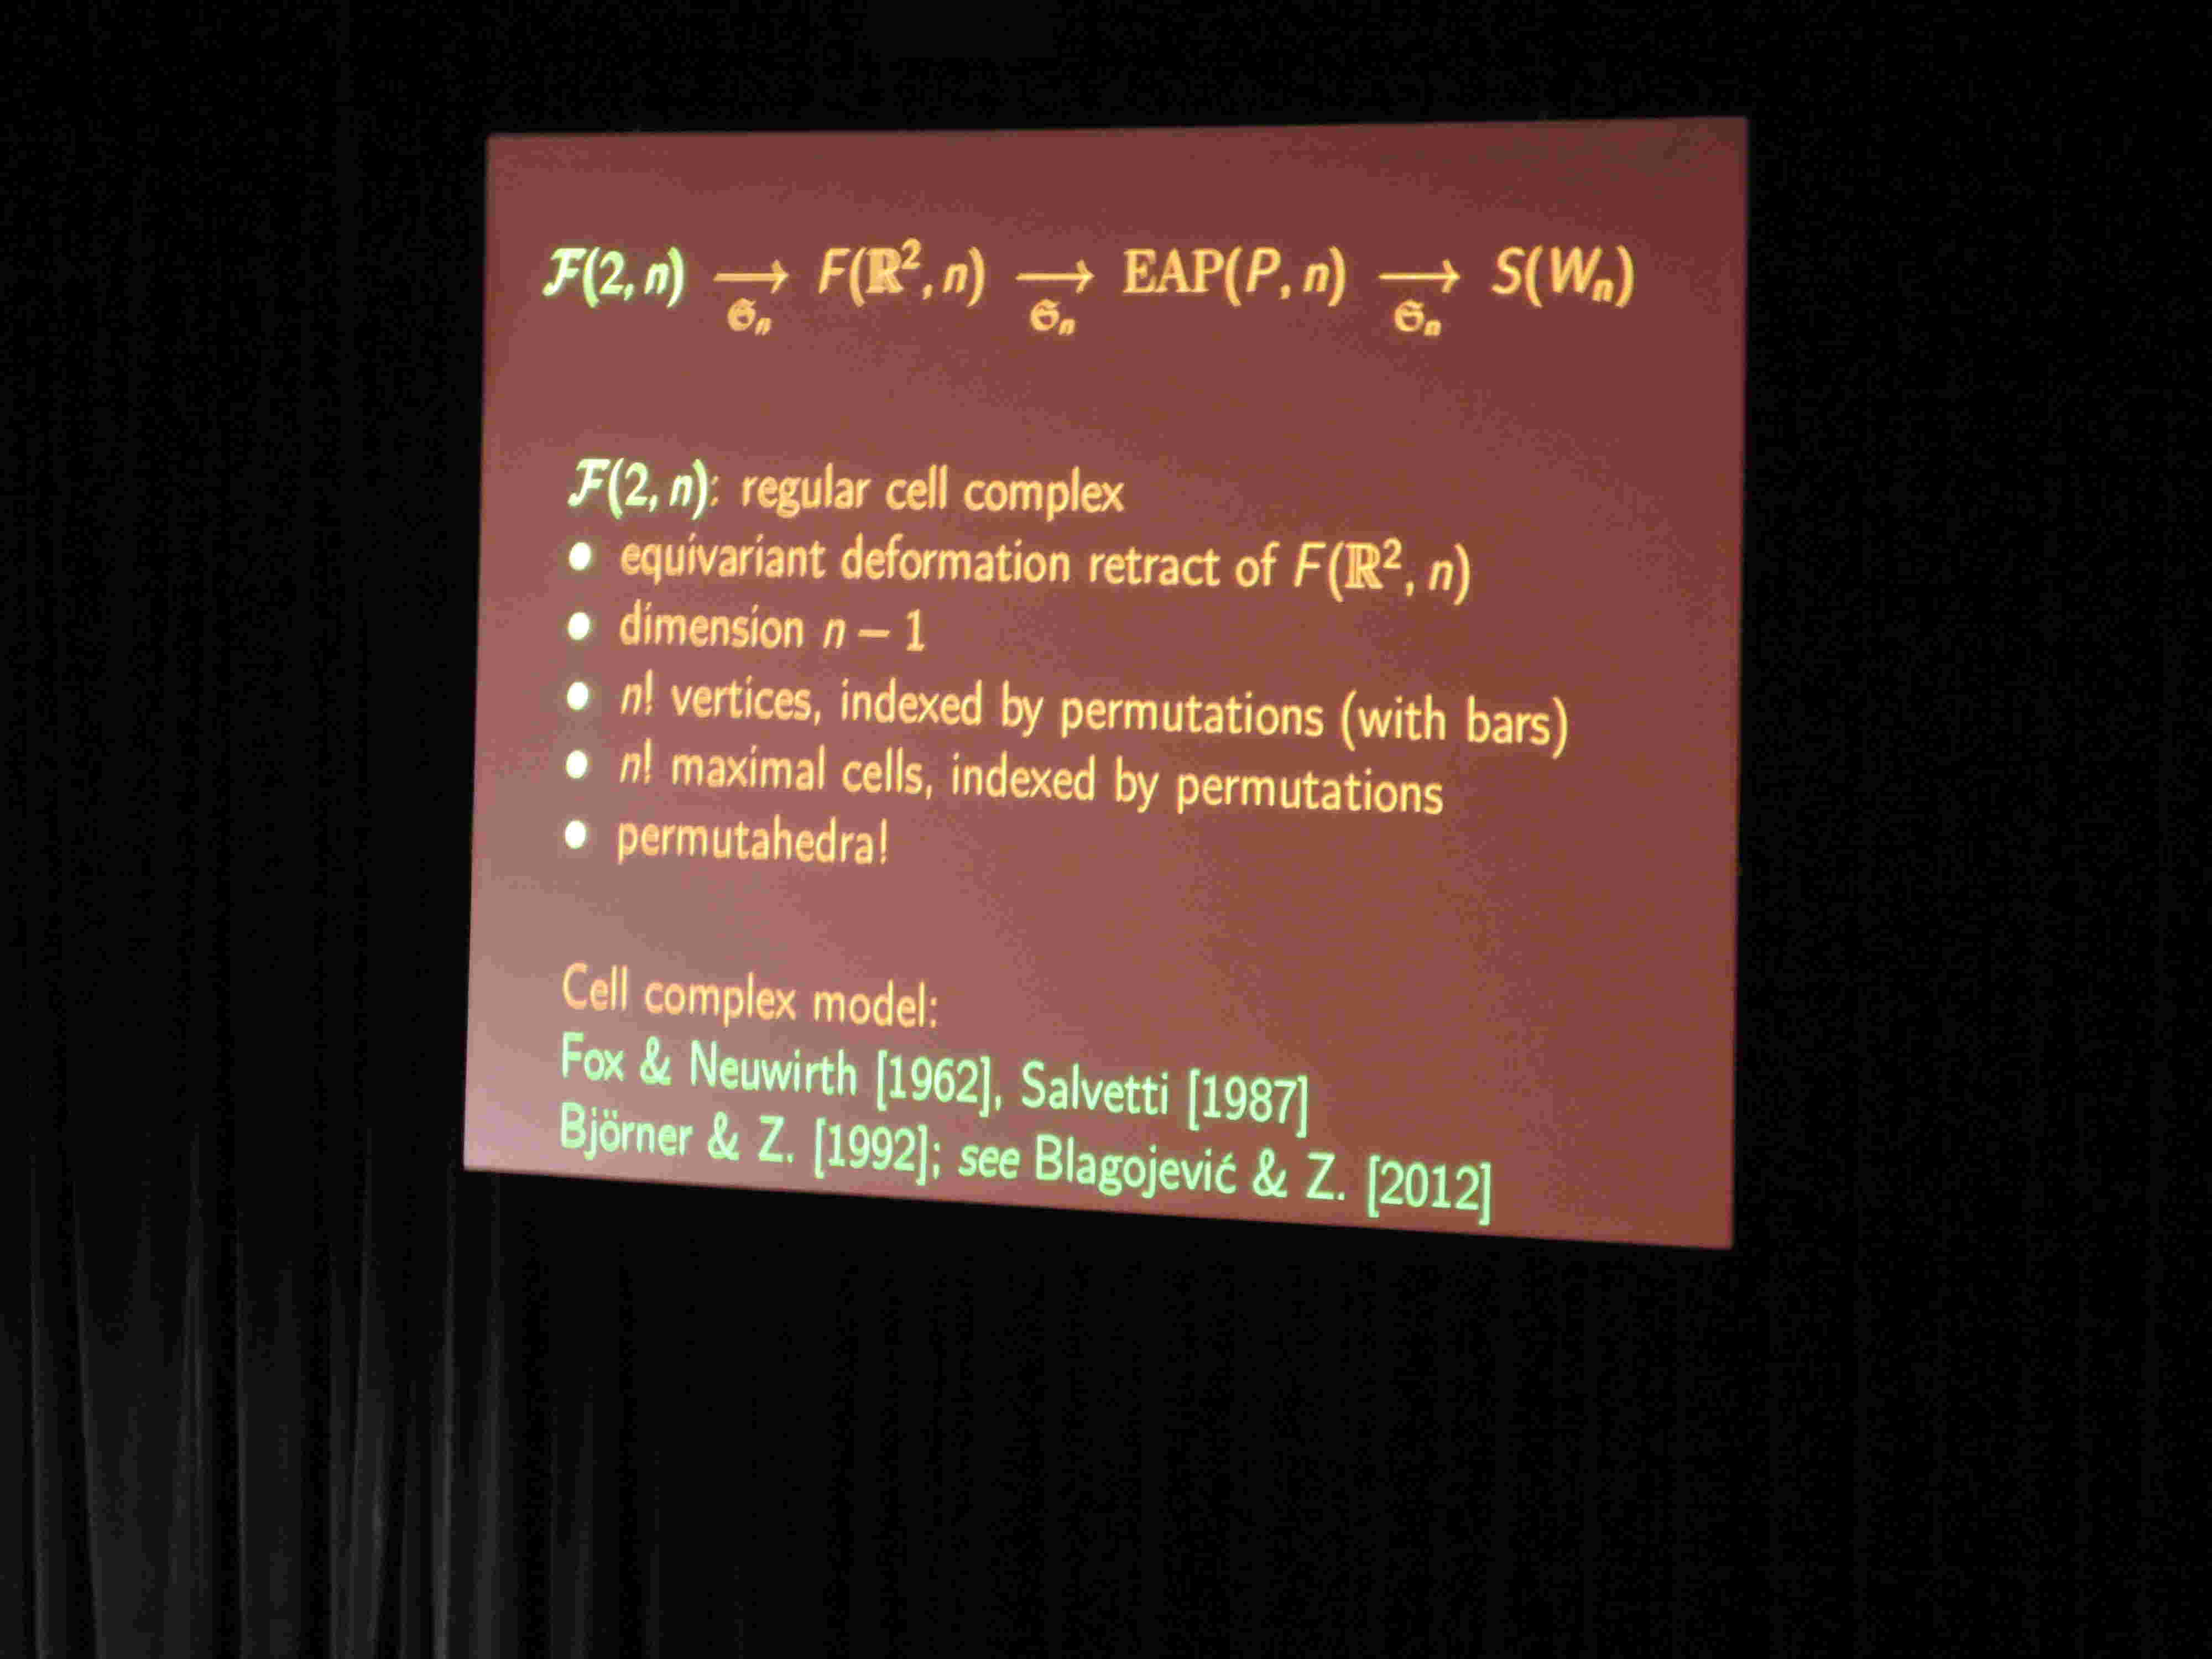
\includegraphics[width=0.5\textwidth]{media/cellcomplex.jpg}
  \caption{Shooting cannons at sparrows.}
\end{figure}


Thus this creates a continuous map $F(2,n) \to S^{n-2}$ which is equivariant.
However, it can be shown that this map exists if and only if
$\sum_{k=1}^{n-1} \binom nk x_k = -1$
has an integer solution. This is in turn equivalent to $n$ not being a prime power.
Thus this solves the original problem when $n$ is a prime power.

In the title, the ``sparrow'' refers to the problem above, which looks like an olympiad problem,
while ``cannons'' refers the modern weapons that were used against it.
I prefer the term ``bazooka''.

The lecturer uses quite cool mathematics and I manage to grasp the basic line of attack.
But while the math was quite interesting, I find the delivery rather slow and not terribly interesting.
I would have preferred to just read the slides.
The rest of the Taiwan team reports difficulty in following the English.
I suspect the Japan team next to us has the same issue as $\tfrac 23$ of them are asleep by the end
of the lecture.
As a result, we decide not to attend the following lecture on mathematical physics and cosmology,
and return to our dorm for a while.
There seems to be some interesting in the upcoming NT lecture, however.

While waiting for the NT lecture we get ambushed by housecleaning services, which replaces our linens and towels,
among other things. A few minutes later we realize we are actually late for the lecture and the Taiwan team opts
to ditch. I suspect that Apollonian circle packing is going to be similar to one of Palmer's CHMMC power rounds anyways, so
at least I don't miss out on too much. I do in fact go over and see if the lecture still has open doors, but it does not.

At around noon, Po-Sheng and Pang-Cheng and I decide that it is time to get lunch; the rest of the Taiwan team decides to continue watching
anime, which as usual I still cannot understand.
As was bound to happen eventually, it is around this time that I manage to get myself locked out.
However, I manage to evade the fee of R30 by asking the housecleaning on the adjacent floor to unlock the door for me.
This was quite happy.

At lunch we run into our team leader who gives us the scores for \#3 and \#5.
No on has lost any partial on \#3, but no one has gotten any either.
Well, things could have been a lot worse.
We have lost a few bits on \#5, much to my annoyance.
However, we expect to lose at most 1 point on \#1, meaning our score is more or less fixed at $192 \pm \epsilon$.

At this point, Dr.\ Hong gives me his Taiwan IMO jacket, for which I am very grateful and would like to acknowledge him here.

We also receive the copies of the problems for TWN2 and TWN6 that were used in coordination.
I now have regained possession of all my contest papers.
I look forward to receiving my contest folder, if that ever happens.

I try to find some company as the Taiwan team is still busy watching anime, so
I go find Baxter. I run into Razvan Gelca at this point and we chat for a bit about the problems and coordination.
It seems like Razvan is quite fond with the Problem 3 at this year's IMO, as the students have found many different solutions.

I again drop by the Games Room and run into Livio Fetahu and Farrell Wu, and we talk extensively about the IMO
and other olympiad things. I then, as promised, show them on my laptop the current draft of my geometry textbook.
I must have bored them halfway through because they leave quickly when I finish.
The Taiwan team is still watching anime, so now I head up to the 10th floor and visit the Canadian team.
Alex Whatley lets me into his room, where they are playing a game and trying to defeat some snow creature
with around 35000 HP before it makes it all the way across the screen. They fail by 1 HP.
I comment that this does not bode well for medal cutoffs.

\begin{figure}[ht]
  \centering
  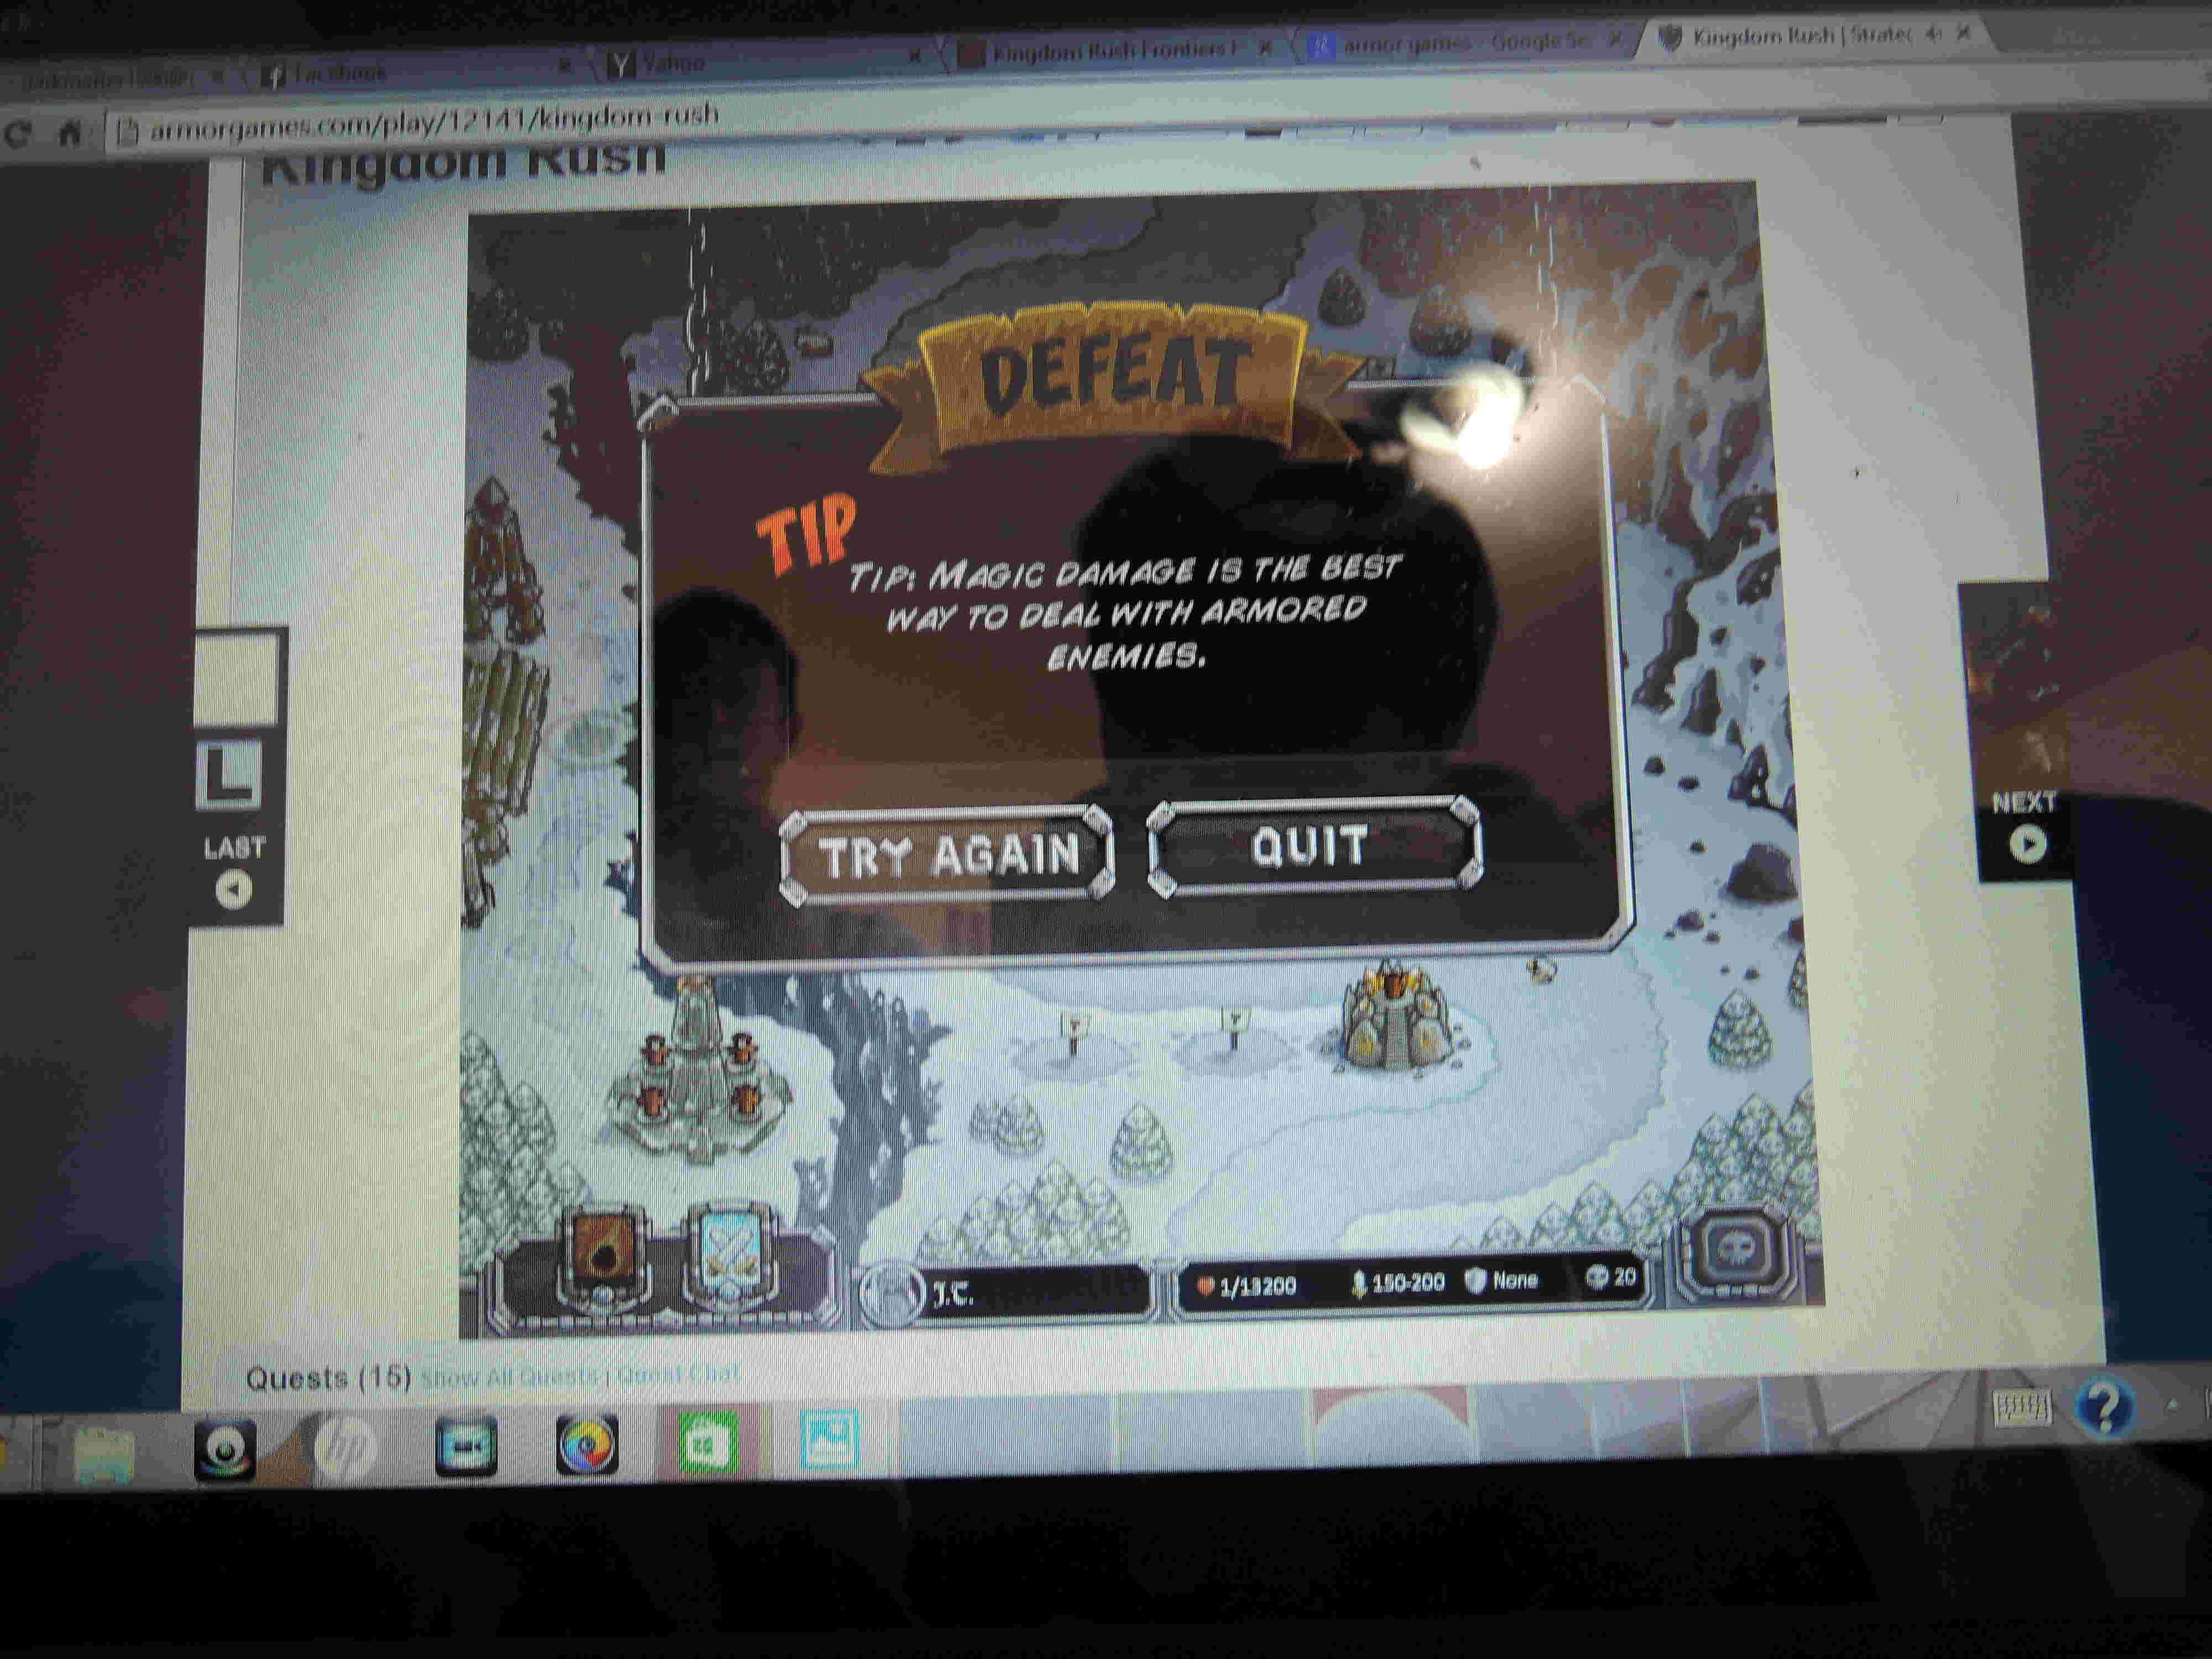
\includegraphics[width=0.5\textwidth]{media/1hp.jpg}
  \caption{Team Canada losing a game.}
\end{figure}

Kevin Sun tries to enter the room, but Alex Whatley refuses to allow him in, on the basis that the previous
three occasions in which Kevin entered, the first led to Kevin stealing his charger, and the other two led
to the entire US team rushing inside.

However, at this point a large number of projected scores materialize.
Antonio Molina from Canada has evidently taken photos of the current coordinated scores,
and has assembled them in a spreadsheet
and is trying to determine the range of ranks that Canada might obtain.
I ask for a copy of the spreadsheet as well, and return to the Taiwan team to discuss what our ranking might look like this year. I insist
we are presumably top five.
Our deputy leader then arrives and informs us that we are almost certainly placed third, modulo the Russians.
As it turns out, the Russians will trail us by only one point.
The large screen with the scores on the first floor of Leo then becomes updated with the most recent standings
and so we now have near-complete information, modulo the bulleted scores that arise each year.

At this point I think I lock myself out again. It actually turns out that my key was being sat on
by a pillow in Room 406. There went the first R30 that I spent at the IMO.

It is now approaching 7PM, and the entire Taiwan team plus observers now takes a trip to the Conservatory
for a fancy dinner at a restaurant called the Conservatory.
The car ride there is somewhat long, and is disorienting because the drivers are driving on the left side
of the road.
We arrive and take several pictures, and are handed some plaque.
As I find the drinking age is 18, I take my first sample of red wine. It is so bitter I do not touch it again.
% Adjacent to me, Ting-Wei seems to enjoy the wine much more. I fail to understand.
Meanwhile we enjoy stealing flatbread from TWN6.

The dinner takes a large amount of time, and eventually Po-Sheng falls asleep completely.
By the time we load onto the car everyone is either asleep or half-asleep.
It is around 9PM, so this does not bode well for the 10PM talk that Po-Shen Loh has on $c>1$.

In the end only Po-Sheng and I attend Po-Shen's talk.
Unfortunately, the jury meeting with the leaders is delayed, so in fact Po does not arrive until around 10:40PM.
During this time, the official results appear on imo-official, and the crowd explodes in a frenzy of phones
as we check results.
I find that my score of 36 has won me 12th place, and more importantly, is strictly higher than all the scores
of the US team members. I have accomplished one goal for this IMO.
Moreover, Po-Sheng's perfect score has been confirmed.
I then chat with the US team and Alice from Hong Kong about various things until Po arrives.

The talk is ridiculous.
Let me see how much of it I can still sketch.
First, Po recaps the short solution to this year's IMO6.

\begin{figure}[ht]
  \centering
  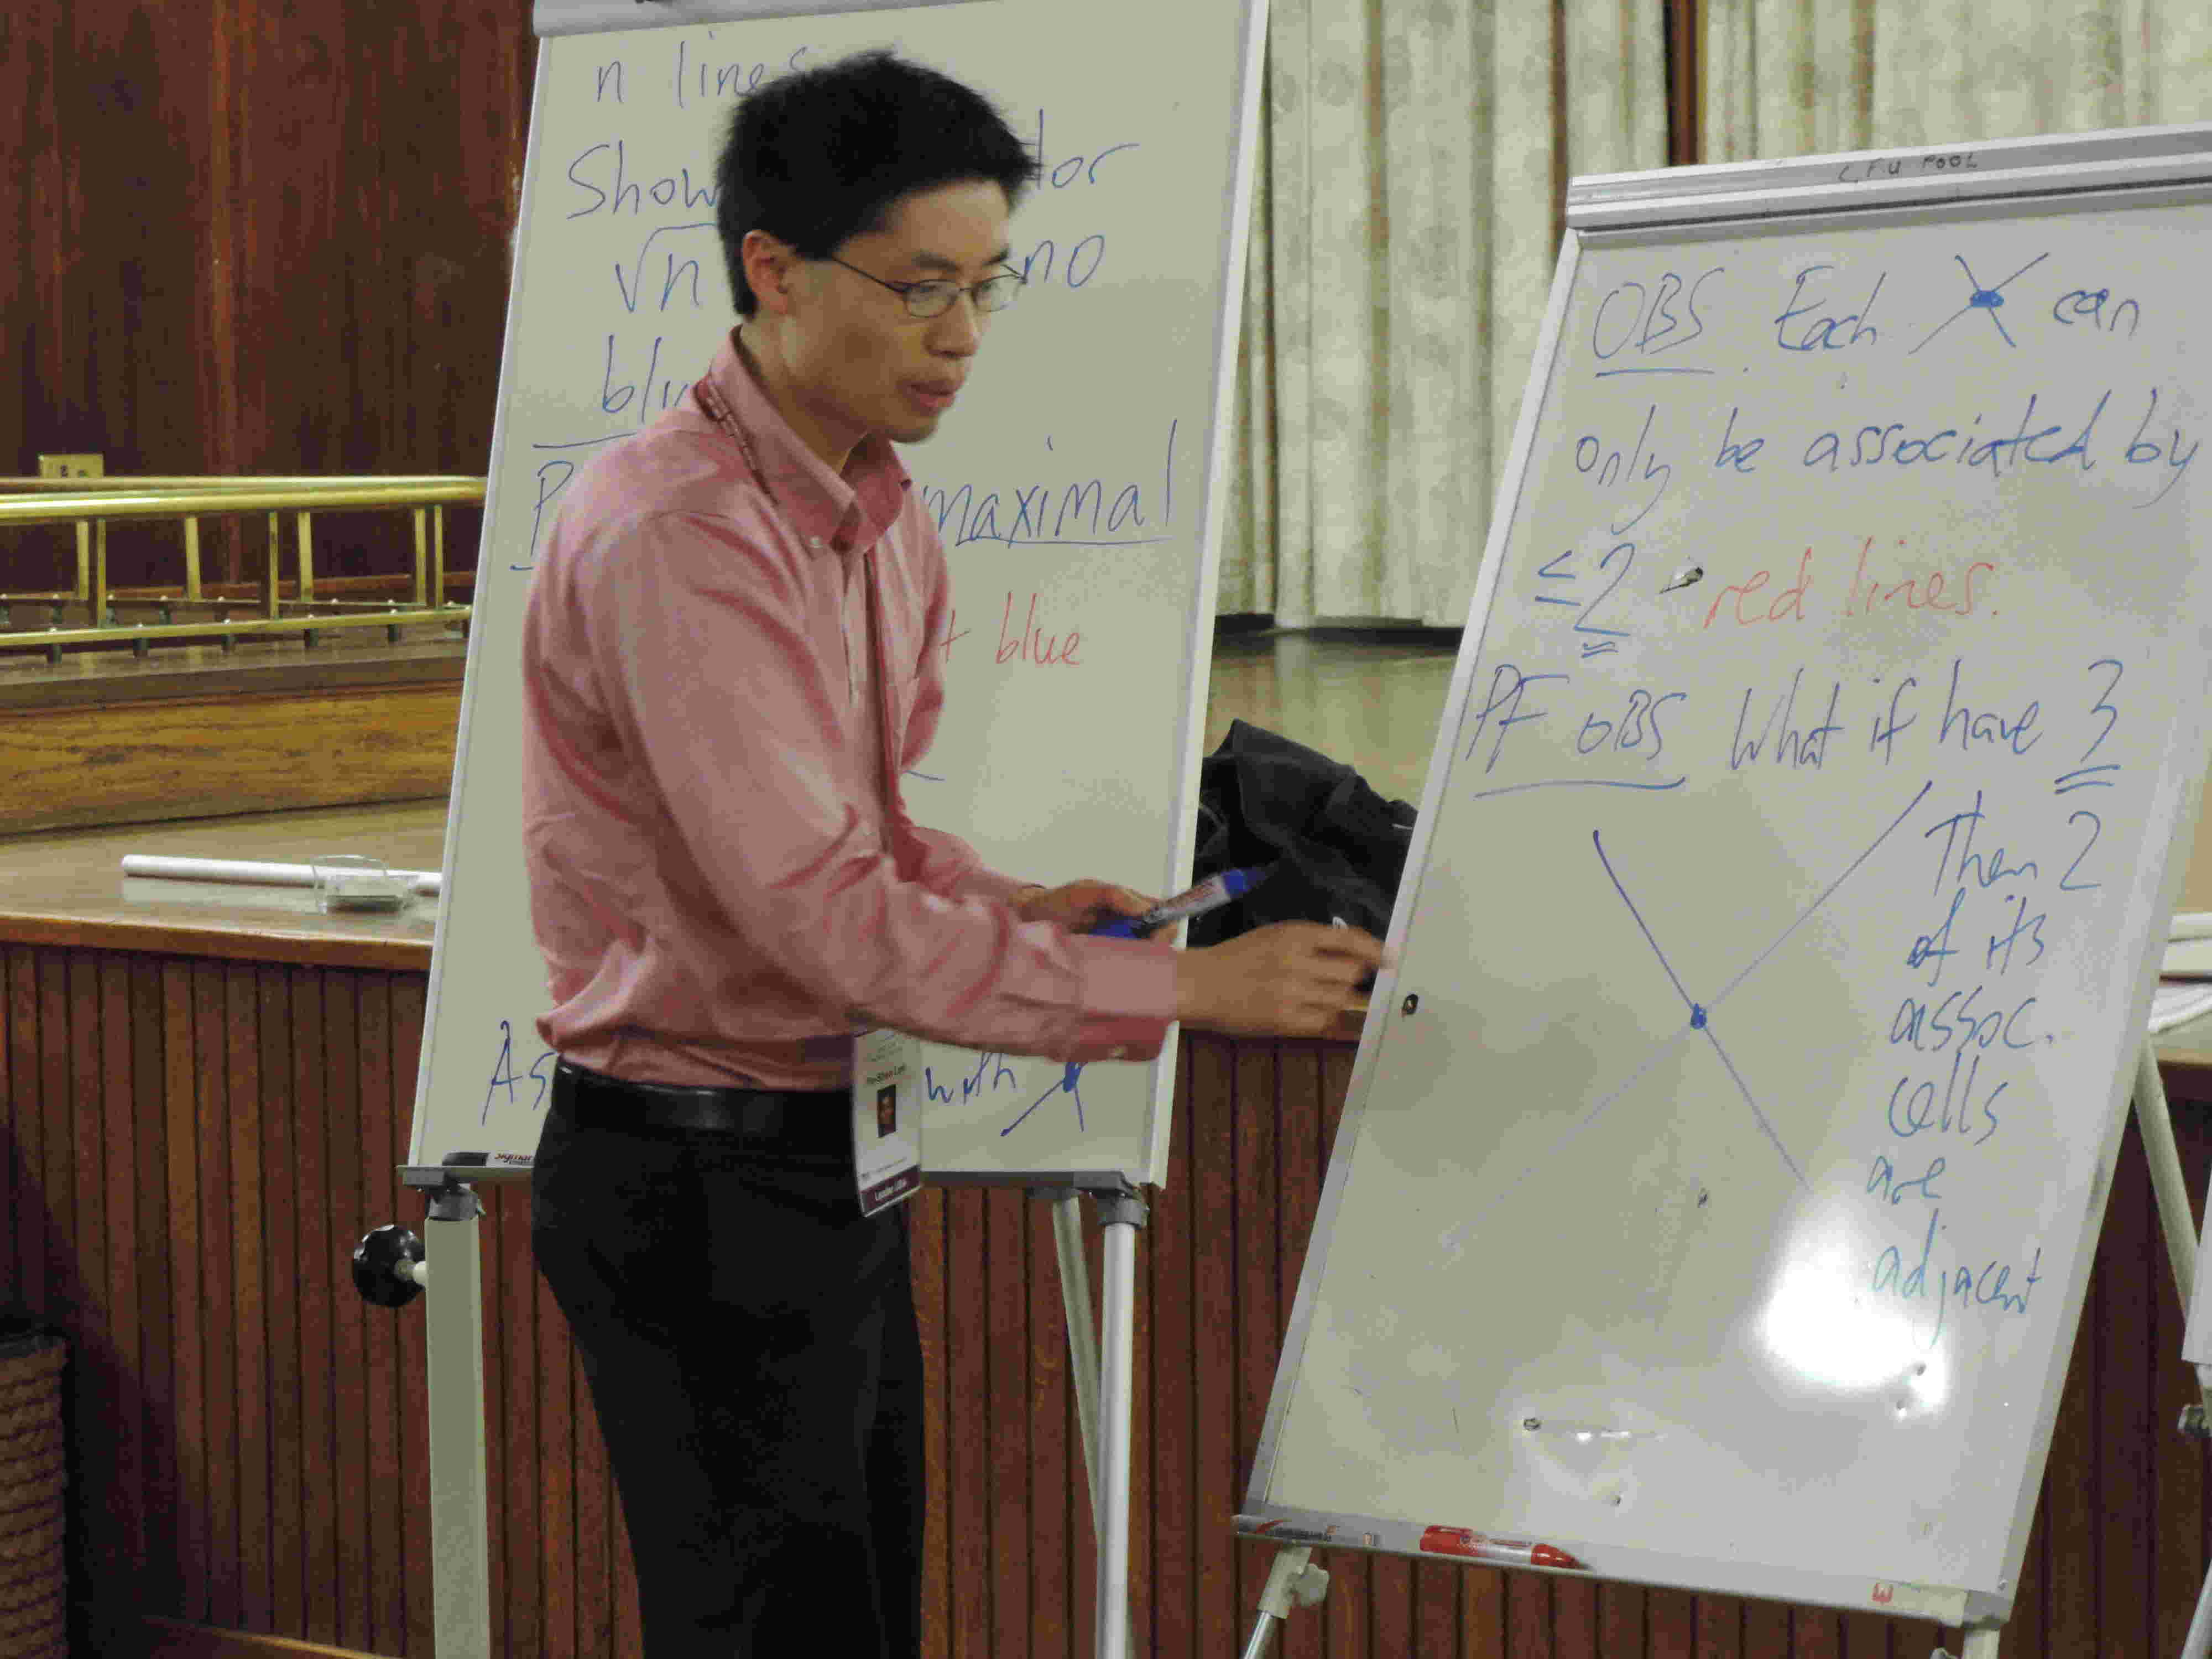
\includegraphics[width=0.5\textwidth]{media/po.jpg}
  \caption{Po-Shen solves the IMO problem.}
\end{figure}

Secondly, he presents the following proposition.
\begin{proposition*}
  Given a graph $G$ with maximal degree $\Delta$ there is an independent set of size at least $\frac{n}{\Delta + 1}$.
\end{proposition*}
One can derive the following as a result.
\begin{proposition*}
  Given a graph $G$ with average degree $d$ there is an independent set of size at least $\frac{cn}{d}$ for some $c > 0$.
\end{proposition*}
The proof is to simply note that at least half the vertices have degree at most $2d$, and apply the original proposition.
Po also presents the probabilistic proof, which uses a ridiculous trick called \emph{sparsification}.
\begin{proof}
  Consider a coin flip $p$ used to pick each vertex.
  The EV of the number of vertices, $X$ is $np$.
  The EV of the number of ``bad'' edges, $Y$, is $\half nd \cdot p^2$ (here $\half nd$ is the number of edges).
  Now we delete a vertex from each bad edge, so the EV of the remaining thing is $E[X-Y]$.
  Pick a value of $p$ to obtain the result.
\end{proof}

Next, we observe a theorem.
\begin{theorem*}[Ajtai-Koml\'os-Szemer\'edi]
  Given a triangle-free graph $G$ with average degree $d$, we can find an independent set with size at least $cnd^{-1} \log d$.
\end{theorem*}
Alon \& Spencer has an elementary proof, but it is very tricky.


Then, we consider hypergraphs. It turns out the following hard theorem exists.
\begin{theorem*}[Duke-Lefmann-R\"odl]
  Given a hypergraph $G$ with $N$ vertices and with edges all of size $3$, suppose that for any two vertices at most one edge joins them.
  Then we can find an independent set with size at least $c \cdot \frac{N}{\sqrt d} \sqrt{\log d}$.
\end{theorem*}
In the context of the IMO problem, suppose we consider each line as a vertex and each cell (finite region) as an edge.
We can reduce each edge with at least five vertices down to a $4$-edge just to make things easier (and strengthen the conclusion).
As before, we use a coin flip $p$ to pick whether a vertex is chosen.
\begin{itemize}
  \ii Let $W$ be the number of vertices remaining. Then $E[W] = pn$.
  \ii Let $Y$ be the number of $4$-edges. There are at most $n^2$ such edges, so $E[Y] \le p^4n^2$.
  \ii Let $Z$ be the number of pairs $(u,v)$ with two $3$-edges containing both (in the context of geometry, there are at most two such edges).
  Then $E[Z] \le \binom n2 p^4 < p^4n^2$.
\end{itemize}
If we eliminate the situations in $Y$ and $Z$ then we reach a situation in which the theorem can be applied.

Finally, let $X$ be the number of edges altogether remaining. Since each edge has $\ge 3$ vertices and there are $\le n^2$ edges, $E[Z] \le n^2p^3$.

Now, we use the following trick. If we select a random configuration, the probability that $Y > 4p^4n^2$ is less than 25\%. Similarly, $P(Z > 4p^4n^2)$ is less than 25\% and $P(X > 4n^2p^3)$ is less than 25\%, as $X$, $Y$, $Z$ are nonnegative.  Meanwhile, $W$ is a normal distribution, so asymptotically the chance that $W < 0.99pn$ approaches $0$.
Consequently, there is a nonzero chance that all these inequalities fail, meaning $Y \le 4p^4n^2$, $Z \le 4p^4n^2$, and $X \le 4n^2p^3$, and $W \ge 0.99pn$.

\begin{figure}[ht]
  \centering
  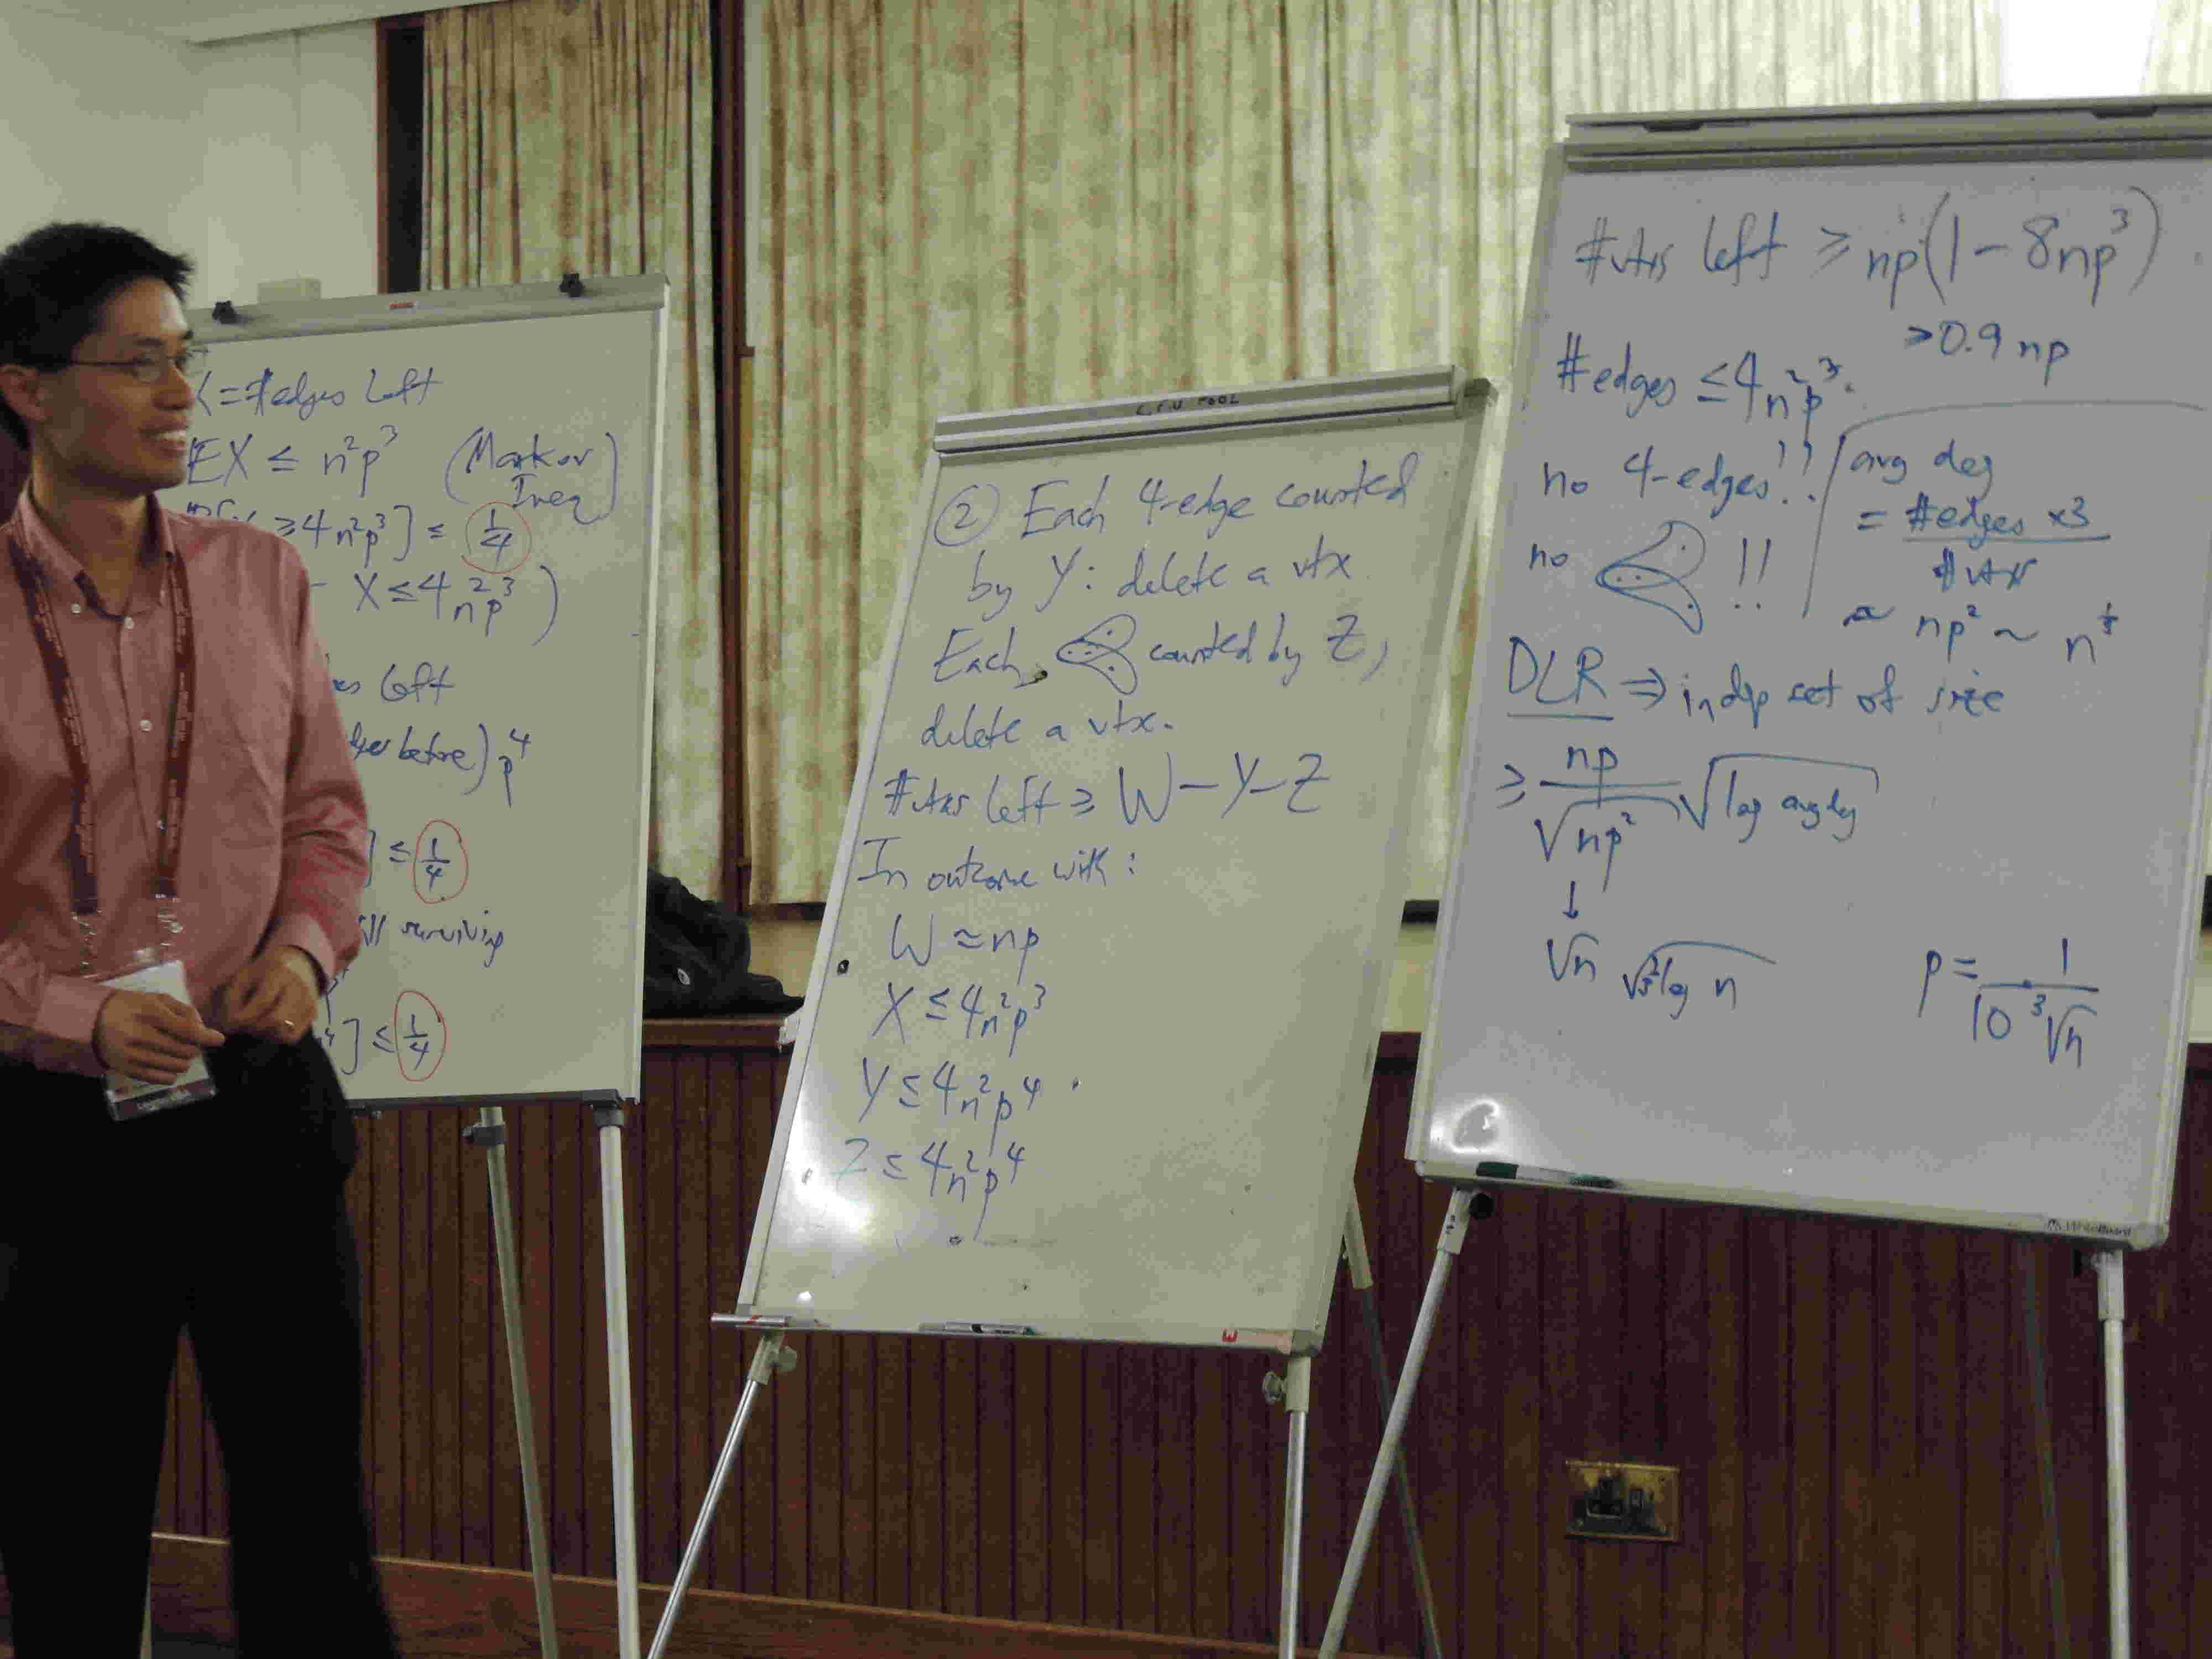
\includegraphics[width=0.5\textwidth]{media/po2.jpg}
  \caption{Po-Shen establishes the bound $\sqrt{n \log n}$.}
\end{figure}

Now using sparsification, delete the ``bad'' situations in $Y$ and $Z$.  Then the number of vertices, $N$, is at least
\[ N \ge W - Y - Z \ge 0.99 pn - 8p^4n^2 \sim pn(1-8p^3n) \]
Let's pick $p = 0.01n^{-1/3}$.  Now $N \sim pn$.

The average degree is at most \[ d = \frac{3X}{N} \le \frac{\sim n^2p^3}{\sim np} \sim np^2. \]
The theorem then gives us a bound of
\[ \frac{N}{\sqrt{d}} \log d \sim \frac{pn}{p\sqrt n} \sqrt{\log \sqrt{pn^2}} \sim \sqrt{n \log n} \]
as desired.

It seems like other people were somewhat lost by the talk.
I loved it.
Anyways, by the time the talk ends, it is already midnight, and so everyone retires to their rooms.
Unfortunately I get caught up in talking to people who are congratulating me and so on.
As a result I fail to sleep until 2AM; not so great for the 7AM breakfast tomorrow.

\section{July 12 -- Penultimate Excursion and Closing Ceremony}
For the first time I am woken up by knocking at my door at 7AM.
Although I somewhat question why it is necessary to eat breakfast at the earliest possible time, I drag myself out of bed and head over to the dining hall.
During the meal, we enjoy a picture on Facebook which shows CBD placed next to Jigglypuff, reproduced here.

\begin{figure}[ht]
  \centering
  
\includegraphics[width=0.3\textwidth]{media/cbd_jigglypuff.jpg}
  \caption{你也是肉墊!}
\end{figure}

We gather at the bus stops at 8:00 AM.
During the previous excursion I had wound up sitting on a bus for 90 minutes wishing I had my contest diary, so this time I decide
to bring my laptop along, of the impression I would be able to leave it on the bus.
Unfortunately, this is false, and I end up carrying my laptop case for the duration of the excursion.
However, I do manage to catch up on my diary to some extent for yesterday on the half-hour ride to the bus.

We arrive at the destination and look for the aquarium for which the entire IMO group has been given free entry.
On the way we run into the Chinese team, and exchange hearty congratulations.
It looks like the Taiwan and Chinese leaders all know each other very well.
I am happy to see what I consider the spirit of the IMO, in which everyone is happy for everyone else's successes.
We take a few pictures and then depart.

The aquarium itself consists of one large cycle and we move through the exhibits.
It is hard to describe in words, but it is certainly quite an enjoyable experience.
There is a particularly fun exhibit in which people can crawl into an aperture in the fish tank.
Here is a picture of Dr.\ Hung inside it.

\begin{figure}[ht]
  \centering
  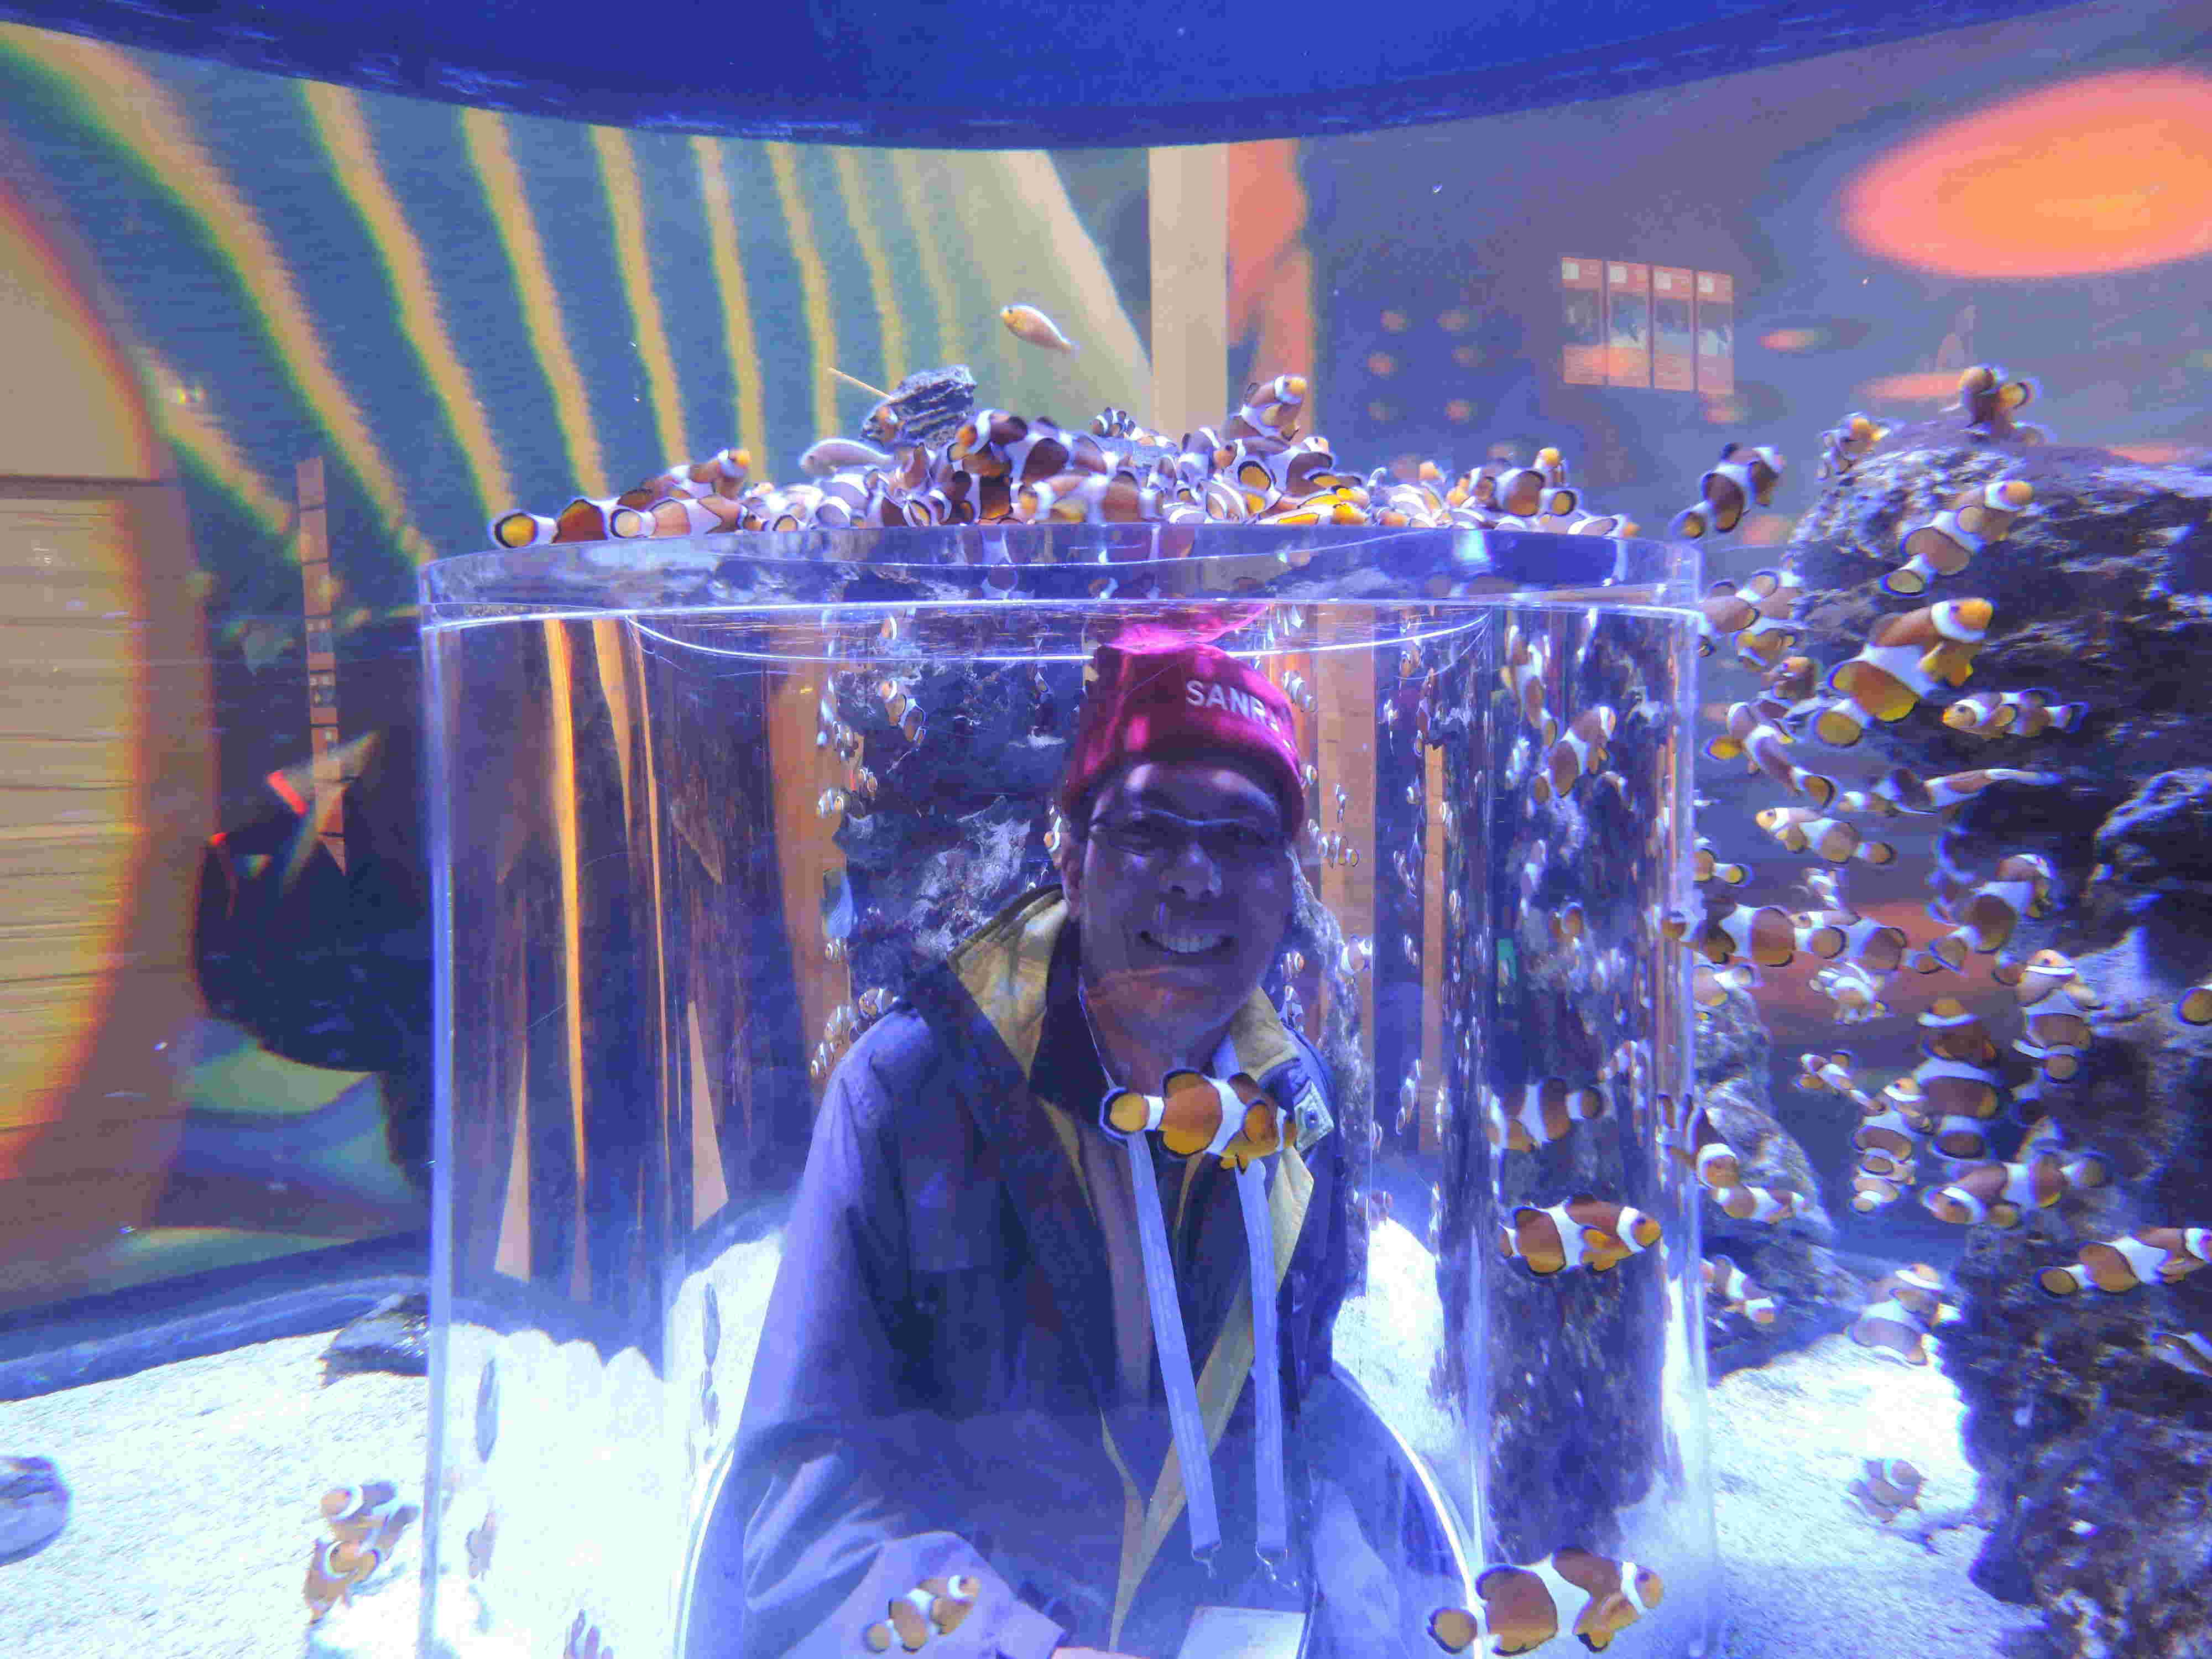
\includegraphics[width=0.5\textwidth]{media/aquarium.jpg}
  \caption{Wen-Liang Hung in a fish tank.}
\end{figure}


At every exhibit we designate any large fish as ``CBD''.
Towards the end of the aquarium, we find a ``feedback'' station which CBD and Ting-Wei proceed to put some troll responses into. I believe they are ``im so handsome'' and ``js turn eyelid''. Anyone who has been with us for more than a few days can guess what the latter refers to.
We then get stuck in the gift store in a flood of people for a while, and on the way out half the team goes to get ice cream.
I think the Taiwan team has been getting a name for getting second meals at the cafeteria a lot, which is ironic since I'm on the team.

\begin{figure}[ht]
  \centering
  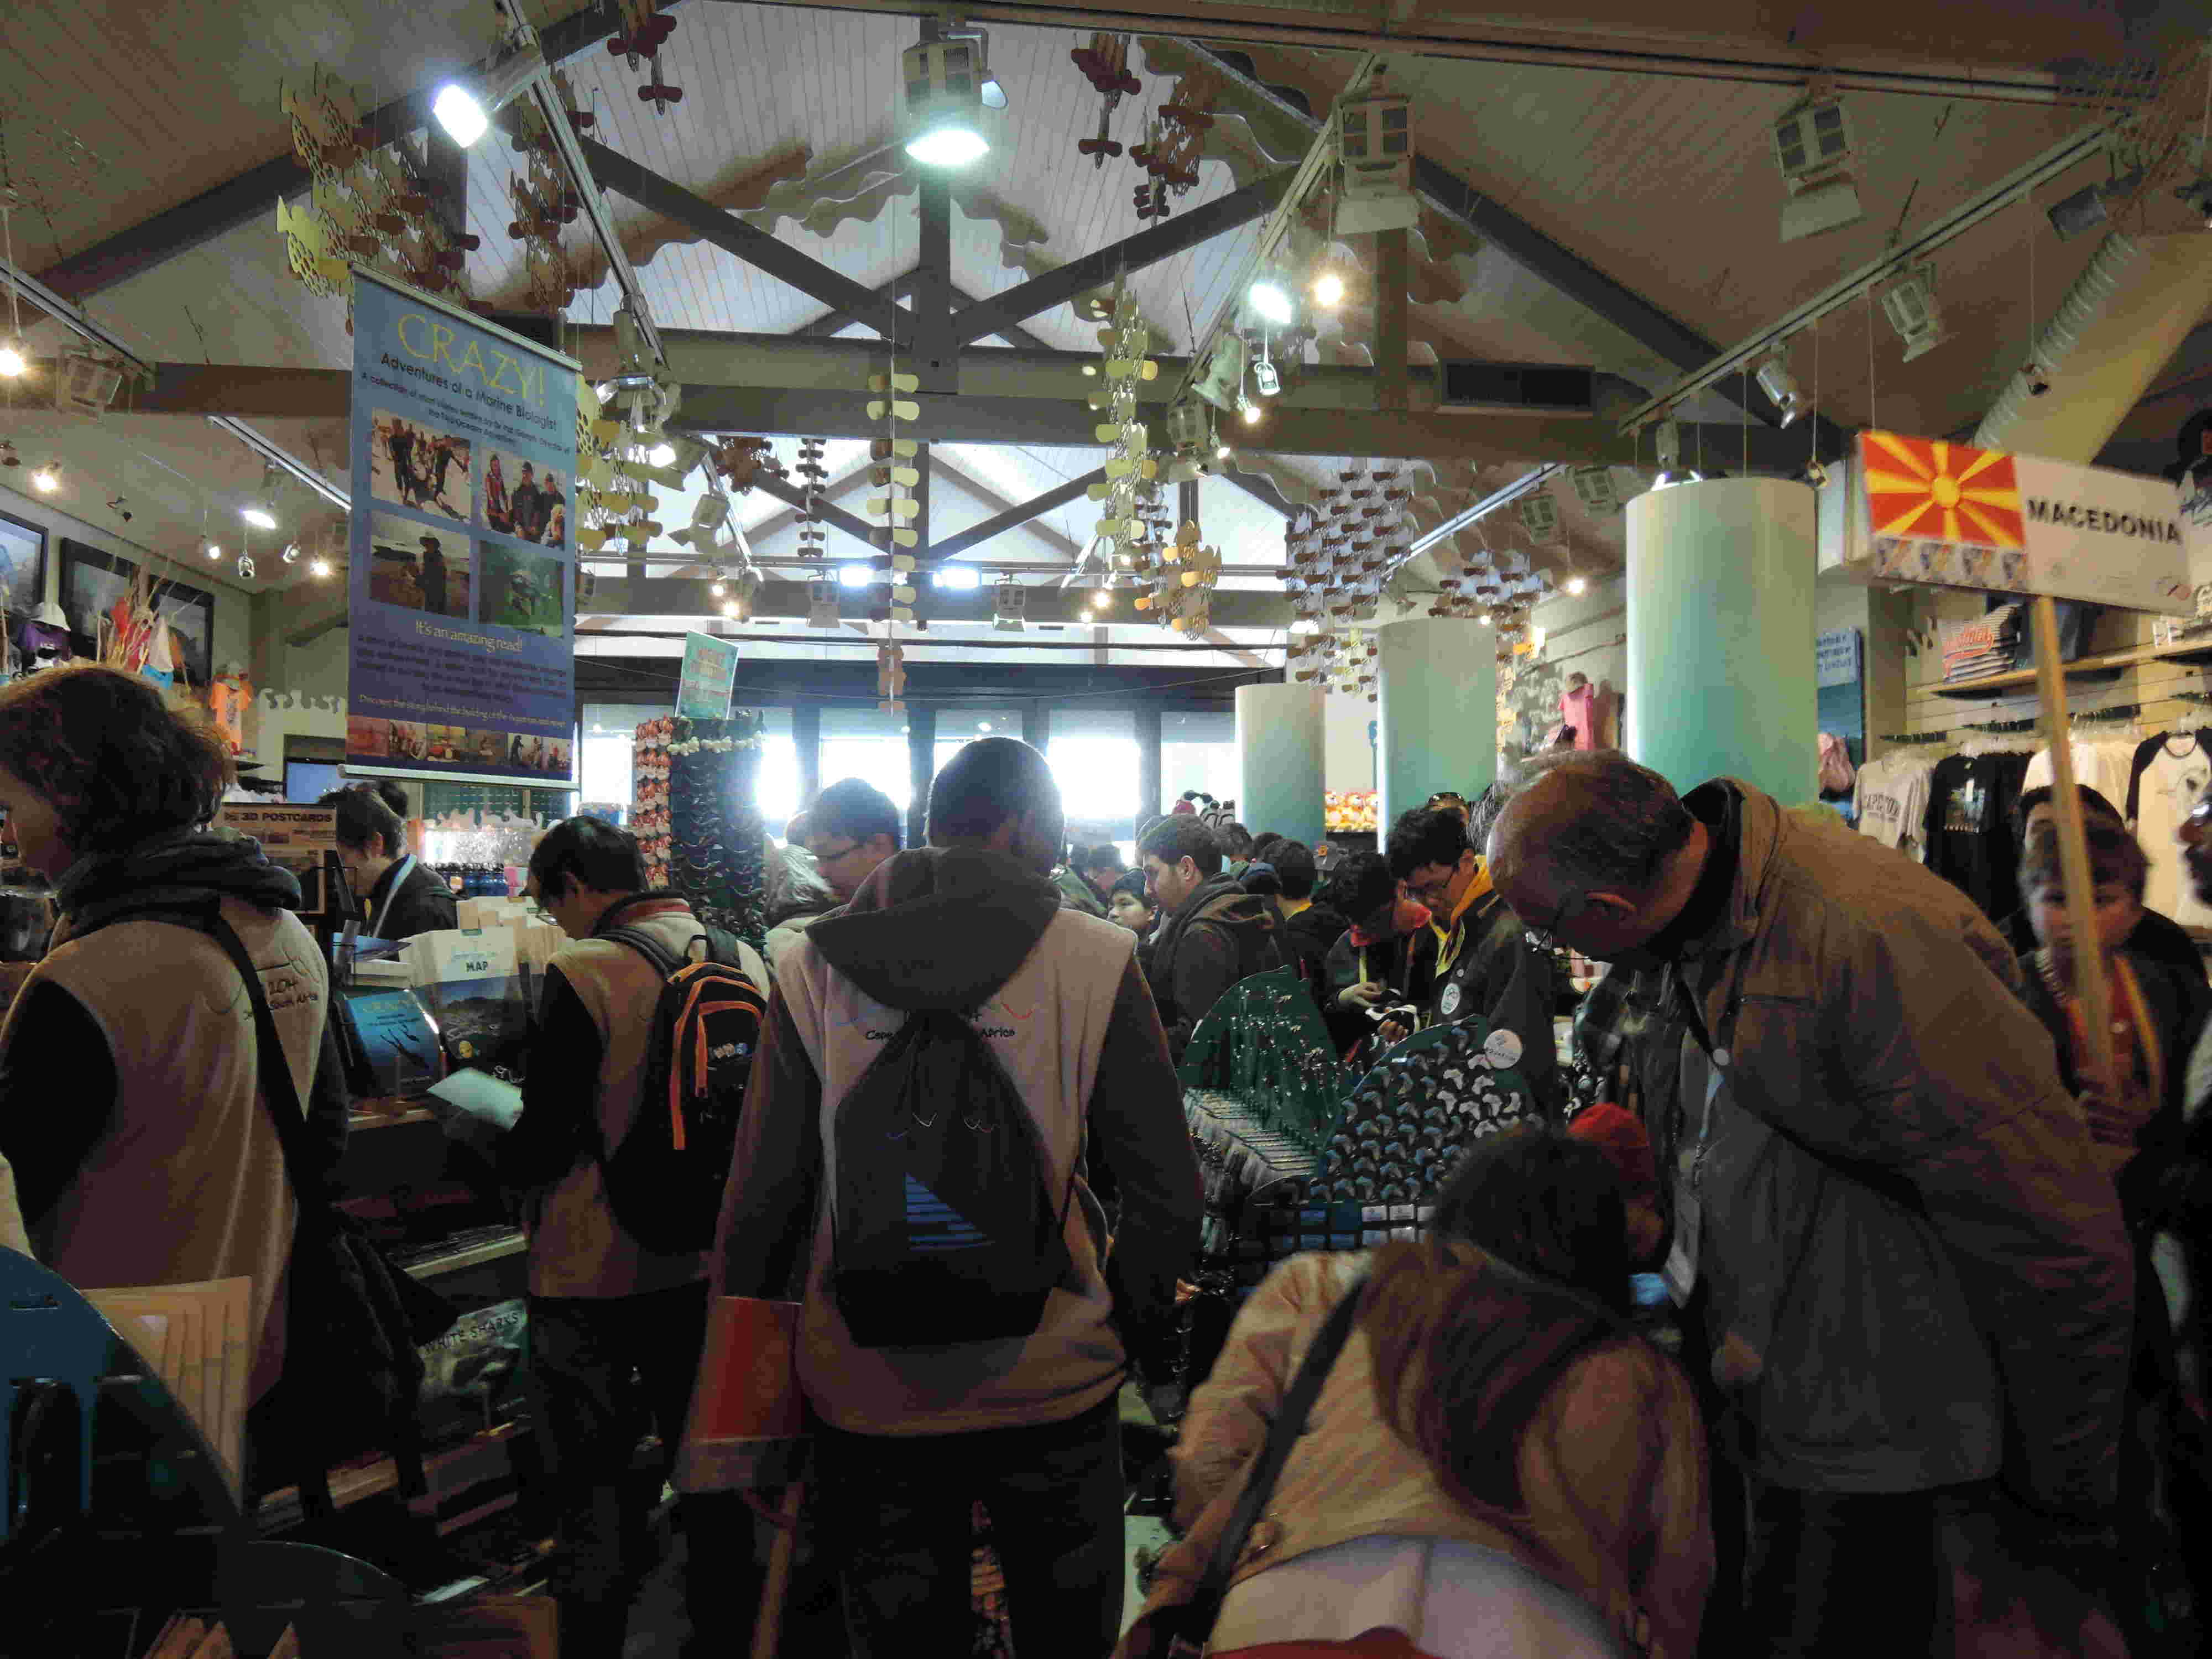
\includegraphics[width=0.5\textwidth]{media/giftshop.jpg}
  \caption{The gift shop at the aquarium.}
\end{figure}

At this point for some reason we return to the aquarium to watch penguins being fed.
This is a long wait, and I get bored halfway through. I also feel tired enough that
I don't actually watch the penguins getting fed.

We then go outside, where my parents are waiting and take even more pictures than I do.
Our sack lunch doesn't seem particularly appetizing, so we basically just eat the chips and dessert,
and then decide to go order sushi. Being the prolific eater than I am, I don't actually eat any sushi.
During this time I try to explain to CBD what Po-Shen had talked about yesterday, but continuously
stumble over myself and therefore don't do a very good job.
However, in doing so I complete the holes in my understanding,
so I will probably write the whole thing up nicely at some point.

Ting-Wei starts talking about inversion again, and I remember him commenting that he wanted problems
which were trivialized by inversion a few days ago. The way to find such problems, of course, is to
invert trivial problems.

We then decide to play an excellent game: everyone simultaneously points at someone, thus generating
a directed graph on $n$ vertices with $n$ edges. Then a player loses if and only if they are part
of some directed cycle.
After playing a few rounds of this (including a game where everyone loses) the Taiwan team begins
immediately trying to compute the probability of winning, or equivalent the expected value of the
number of losers each round. Our deputy leader berates us for not properly enjoying the scenery.

\begin{figure}[ht]
  \centering
  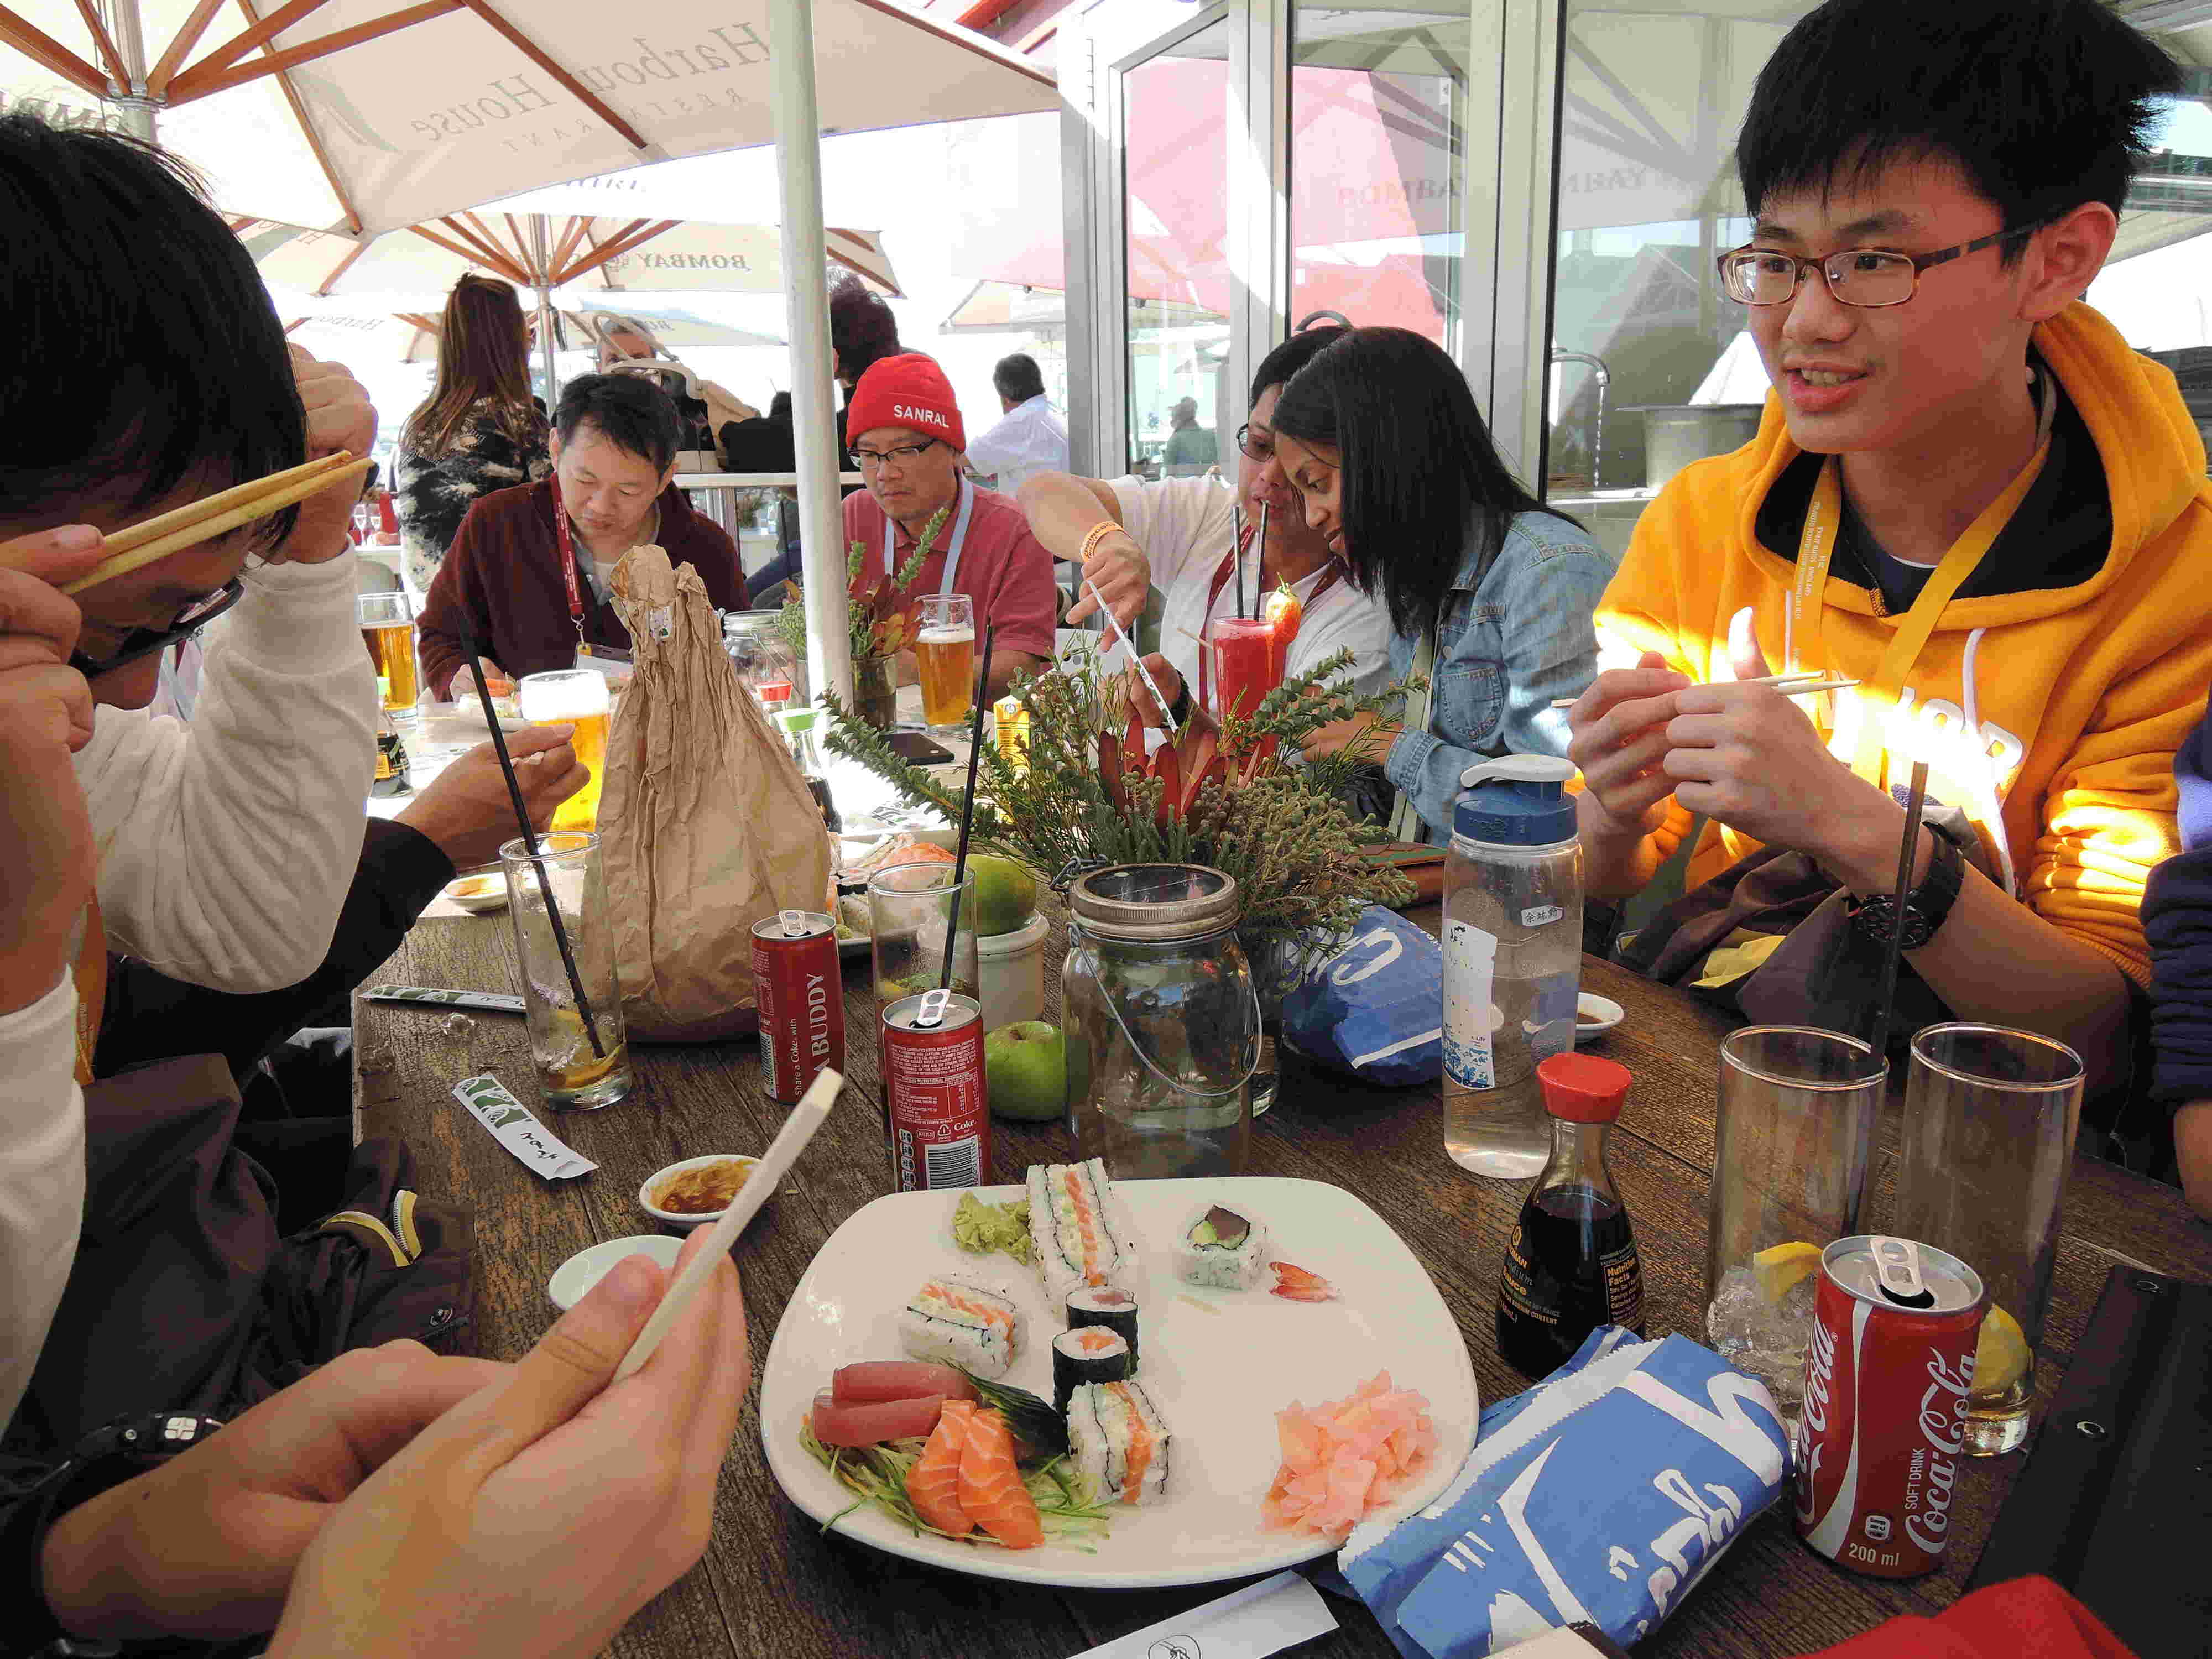
\includegraphics[width=0.5\textwidth]{media/sushi.jpg}
  \caption{Grabbing sushi.}
\end{figure}

By the time this concludes it is around 2:20PM, and the bus leaves around 3PM.
We are asked to meet back at 2:50PM.
Thus we decide to go to McDonalds and order a large fries while continuing to work on this excellent problem.
I regret not ordering more fries.
Anyways the plan almost works, except we end up being a bit late, but so is everyone else.
Right before we leave, some stranger asks to get a picture of us, apparently intrigued by
the presence of a foreign IMO team.

Finally, we return to the dorm via bus and I update my diary on the ride back.
The closing ceremony is to begin at 5:45, and we have arrived back at around 3:45PM.
I take the time to pack a large portion of my belongings while the Taiwan team
reads newspaper articles that have materialized about the Taiwan IMO performance and laugh at their inaccuracy
(one newspaper claimed that the Olympiad was in Colombia and gave the medal results of last year).
We later find on Facebook a comment on a Yahoo news article to the effect of ``this just shows that
Taiwan students are only good at test-taking''. The entire Taiwan IMO team makes a point of liking his comment.

The closing ceremony takes place in the same venue as the opening ceremony did.
All medalists have been sorted into several groups of about twenty each to be seated from outside
(similarly to the seating of teams at the opening ceremony).
Specifically, there are six groups of Bronze and Silver and four of Gold.

Unfortunately, no one seems to knows where anyone else is.
The inability of some contestants to understand English, and the extreme late-ness of the US team, only makes the process more confusing.
As a result, we stay outside for a long while before being properly sorted into groups and entered into the auditorium.
Hung-Hsun comments that last year they had simply labelled the seats with names, and that this had been far more efficient.
I strongly regret not bringing my tablet to play games on.

\begin{figure}[ht]
  \centering
  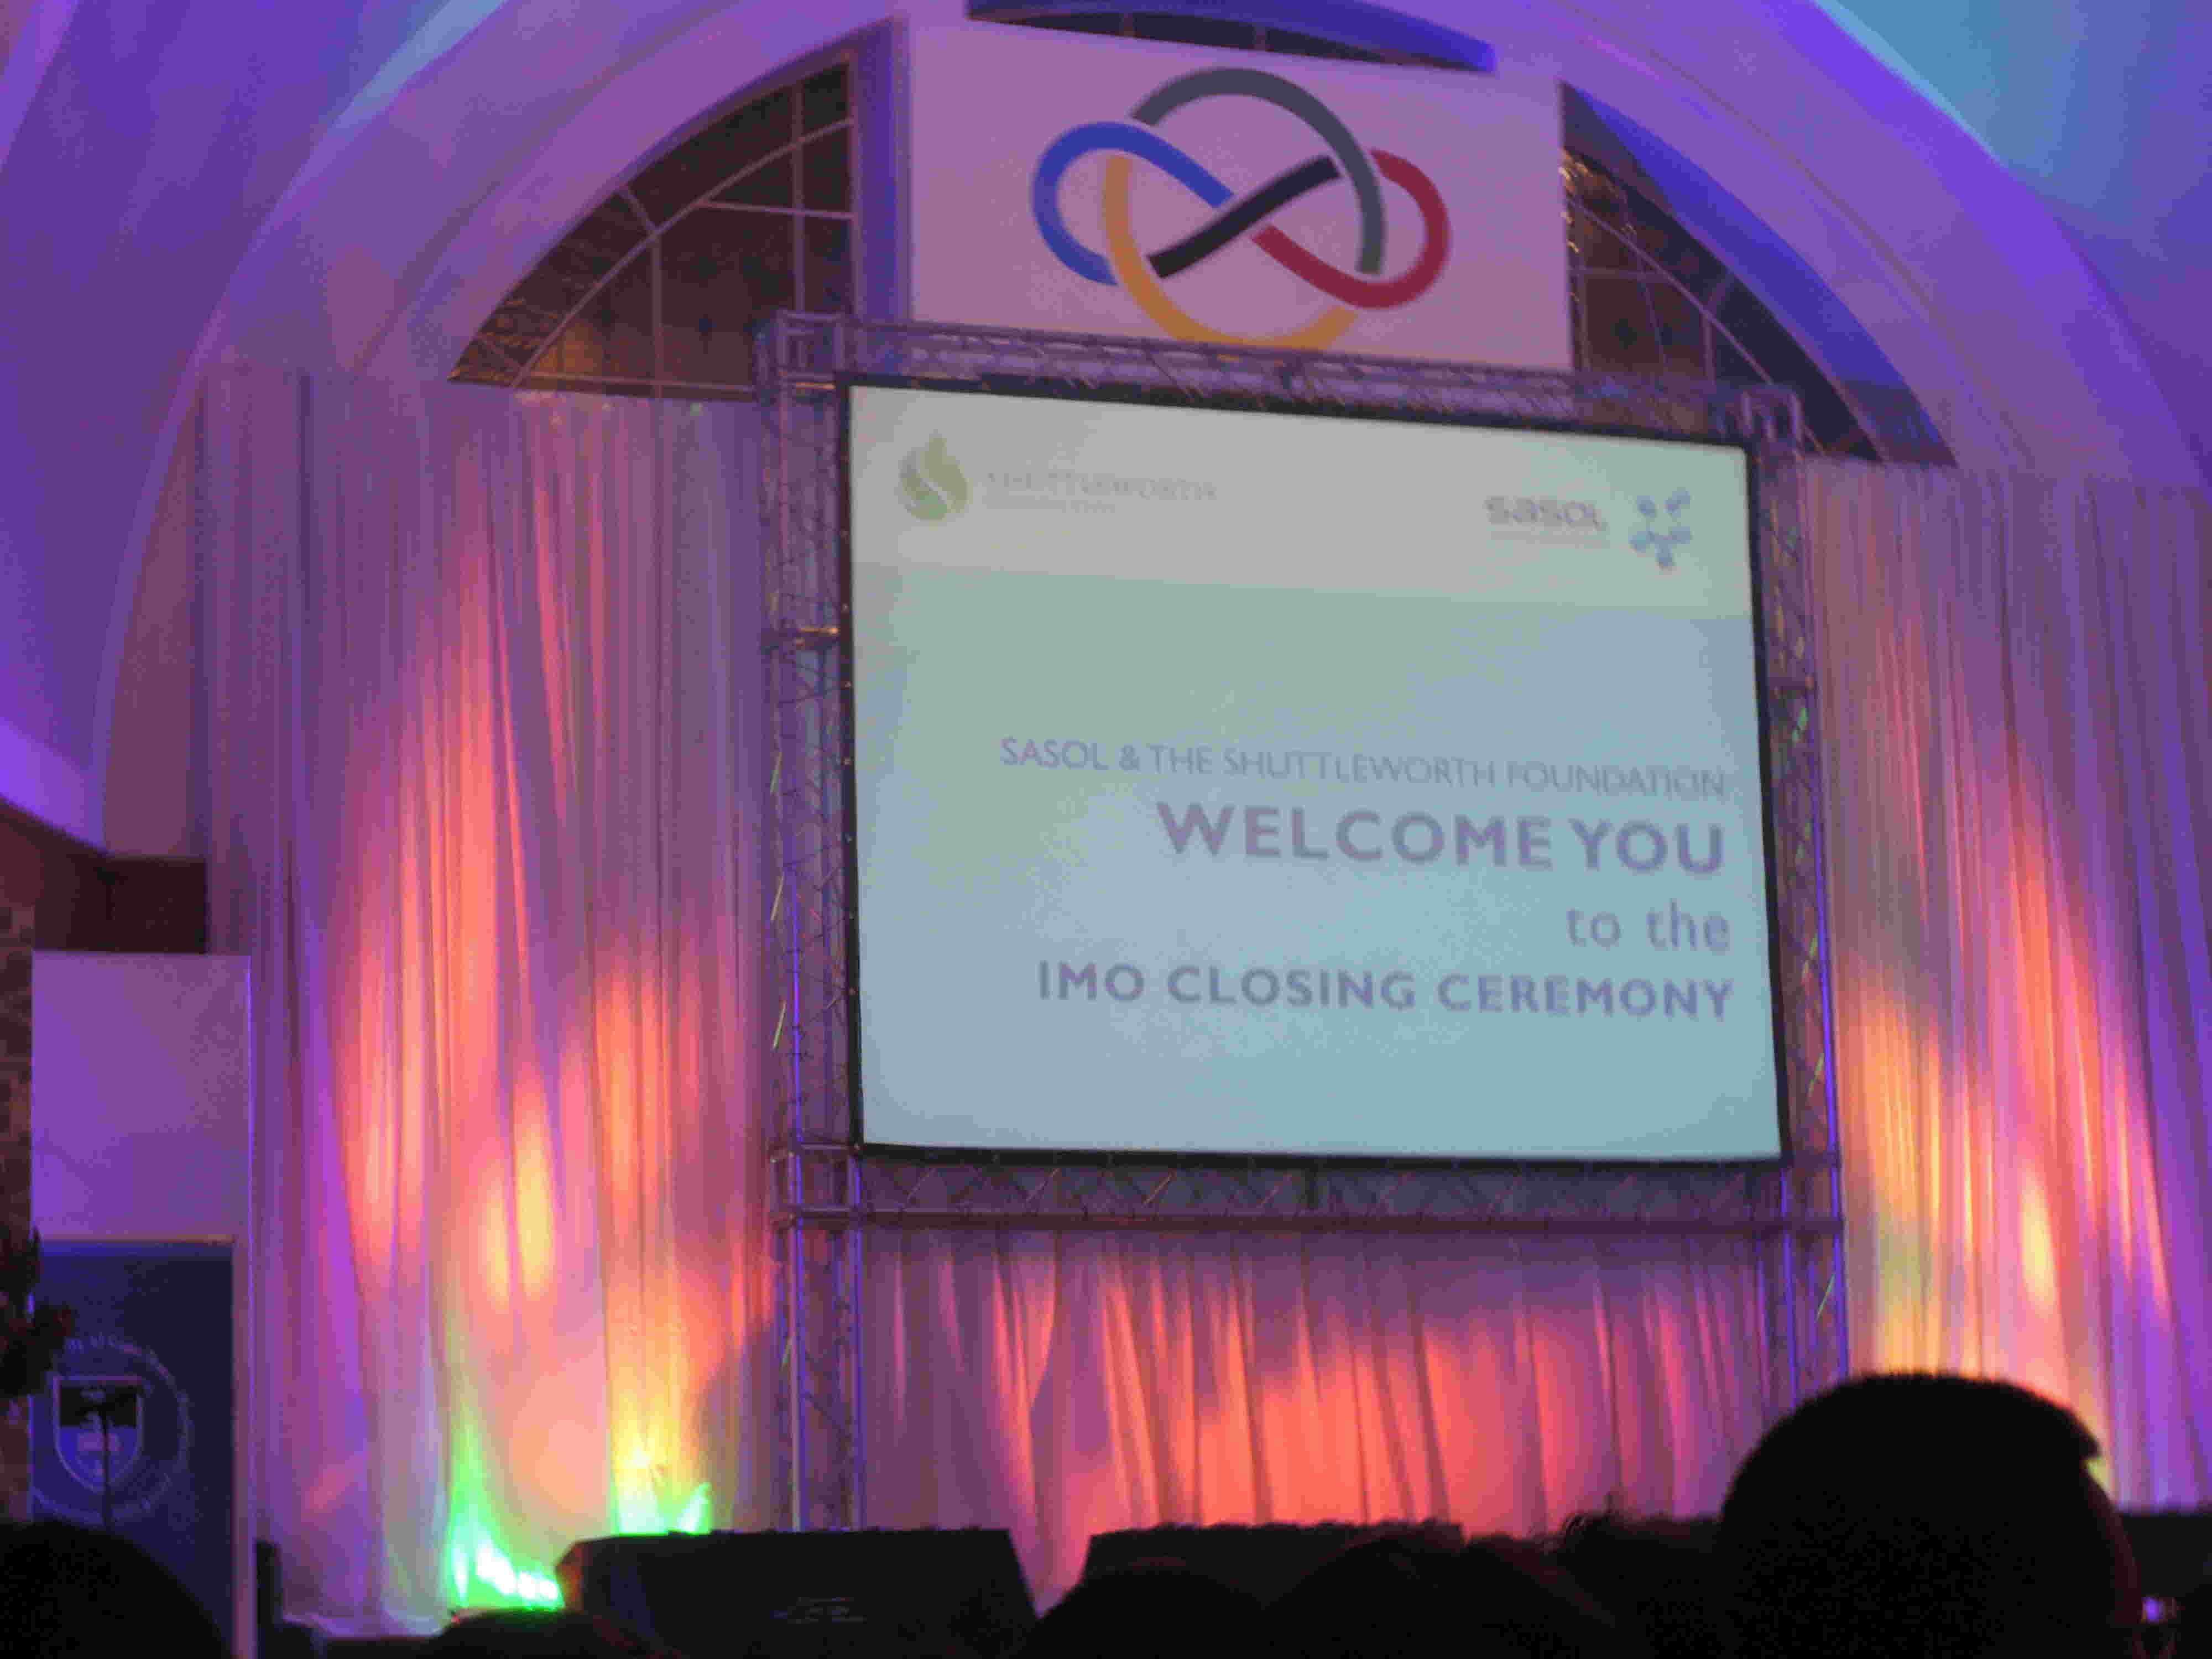
\includegraphics[width=0.5\textwidth]{media/closing.jpg}
  \caption{Closing ceremony.}
\end{figure}

The closing ceremony begins with another performance.
During this time on my iPod, I locate the betting sheet on which USA students had been betting on the results of the IMO.
Some of them I find highly amusing.
In particular, here are the bets on a few events pertaining to me.
\begin{itemize}
  \ii Evan Chen obtains gold -- average 72\%. \\ Bets:
  75 75 75 79 80 60 90 80 60 70 90 70 70 70 95 50 95
  \ii Evan Chen beats all of USA -- average 25\%. \\ Bets:
  21 12 25 43 20 20 17 25 10  5 30 30 20 35 30 30  5
  \ii Evan Chen solves all geometry -- average 59\%. \\ Bets:
  66 37 60 57 60 70 75 70 40 75 60 55 55 50 50 95
\end{itemize}
One person bet 50\% for all events; I have discarded that bet.
I am amused to see that the people who I know personally from MOP 2011 and 2012 have
on a whole placed greater faith in me than those I have not met at MOP 2013 and 2014.
I would like to thank the people who placed significant (greater than 25\%)
probability of me beating the USA team.

At this point we begin hearing speeches, which I have largely forgotten.
We hear a speech from the University of Cape Town chancellor, who makes the amusing remark ``the papers were not easy'',
probably a very strong understatement, and makes a plug for UCT admissions.
Then we hear a speech from the VP of the Sasol Foundation, the Minister of Basic Education, and a
video from the Shuttleworth Foundation. The latter two events do not put me to sleep.

Finally the presentations of awards begins.
Firstly, the names of honorable mentions are projected in large groups for applause.
Neighboring contestant Kevin Sun falls asleep during this presentation.

Then, the Bronze medal presentation team rises to the stage; I recognize some of the names
from the IMO Hall of Fame.
Each group of Bronze medalists (there are many) come up to the stage, one at a time.
Pictures are taken, then at a signal one person from the presenter teams gives the medal, and
they turn to face the cameras again wearing the medals.
Most contestants group with their country, and bring their flag to display for the pictures.

During this time, the Taiwan team devises a scheme to give our perfect scorer TWN5 all the medals so that
when he goes up he will already be wearing five medals. CBD and Pang-Cheng hand over their two Bronze medals
to Po-Sheng.

I then expect the Silver medals to go up, but we have another performance instead, from New World Dance,
before the medals actually resume. Between the silver and gold medals, we have a performance of by a ``traditional
Africa praise singer'' which I don't remember much of, but my notes read ``guy starts screaming'' which basically summarizes
the event. (And it was prose, not song.)

The Gold medals are then presented, for which there are 10 students in the five groups as opposed to the 20 students in silver.
Ting-Wei is in the first group.
I go up to the stage with Hung-Hsun in the second group and we hold up our flag.
Then, we descend the stage and hand the medals to Po-Sheng, who now has all five medals.

At last, the three perfect scorers are awarded their gold medals in their own group, to thunderous, well-deserved applause.
The contestants are Jiyang Gao (China), Alex Gunning (Australia), and Po-Sheng Wu.

\begin{figure}[ht]
  \centering
  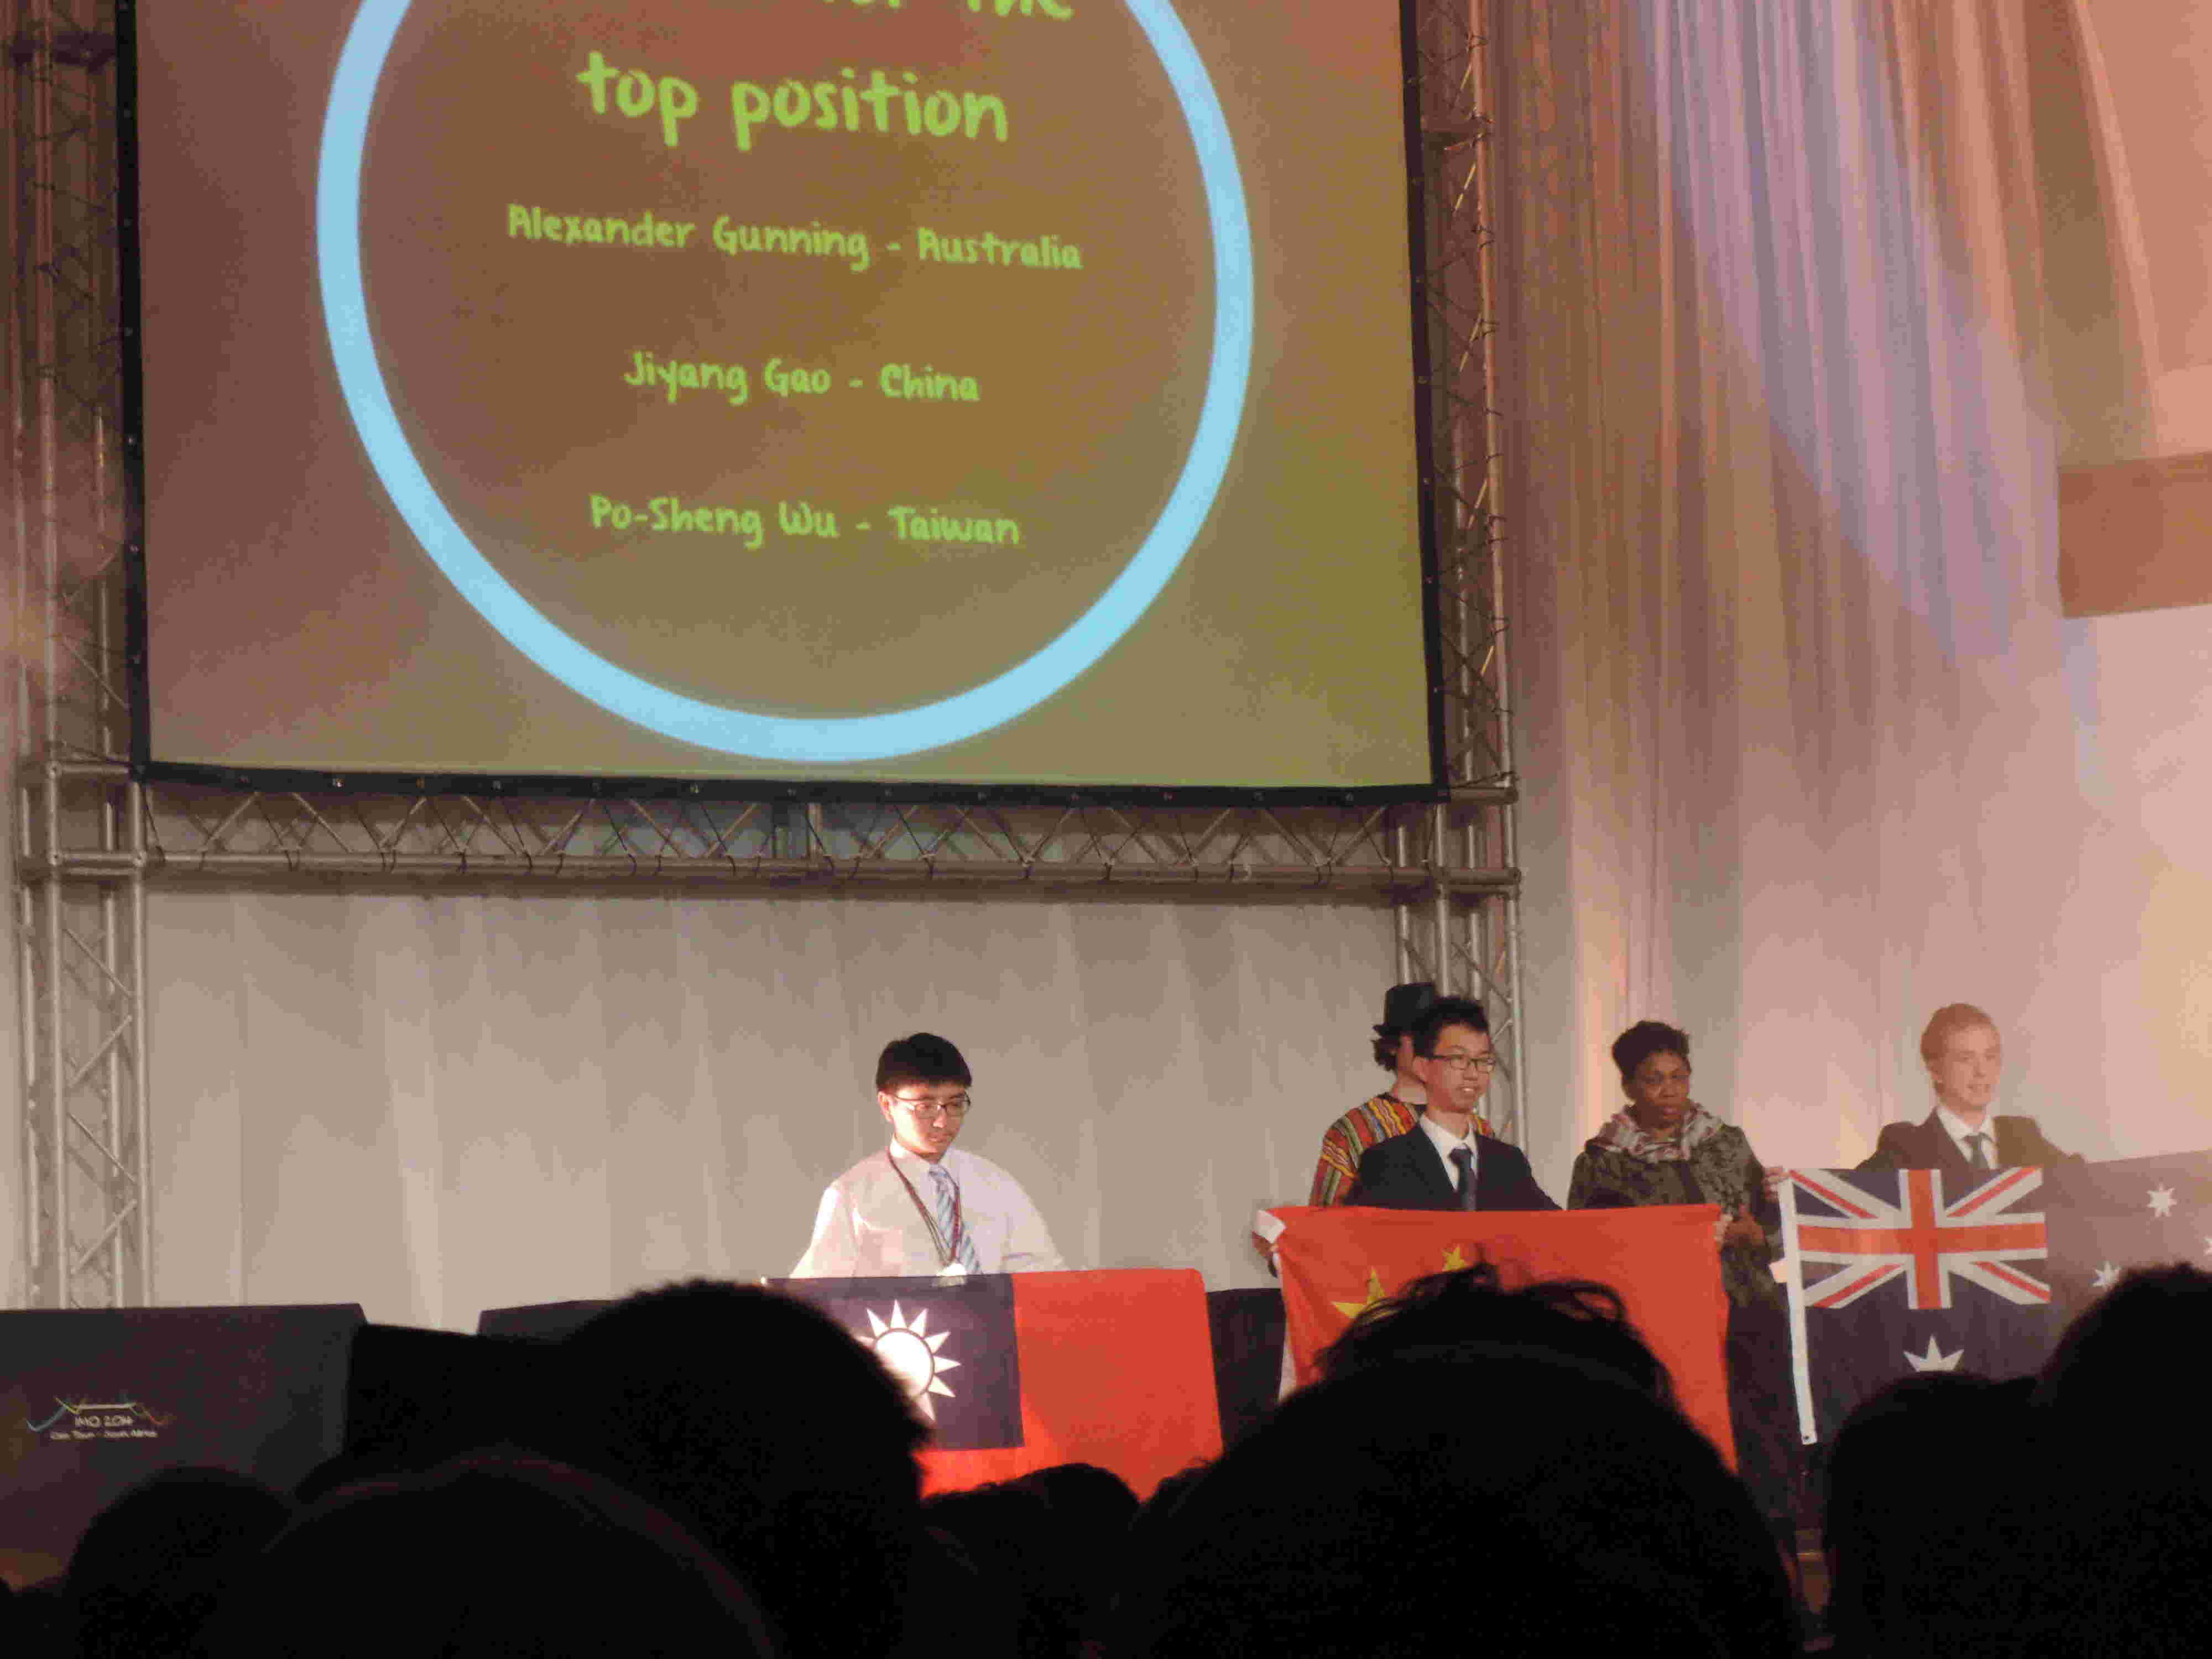
\includegraphics[width=0.5\textwidth]{media/gold.jpg}
  \caption{The perfect scorers.}
\end{figure}

Finally the South African team and the Thailand team are called to the stage.
A video for the IMO 2015, to be held in Thailand, is played,
and the IMO flag is handed from the South Africans to Thailand.
Nazar then formally closes the IMO.

We try to leave, but it turns out that the organizers want a picture of all the medalists
as well as more pictures of the perfect scores, and force the medalists to sit back down.
As usual there is much confusion.
Naturally, they start with Bronze, and so the highest-scoring contestants get dinner last.
Pang-Cheng and CBD ditch the Bronze photo, and then an unnamed mischief-maker on our team (obviously not me)
convinces them to sneak into the Gold photo. No one was tipped off by the presence of six Taiwan students.

Finally we end up in the building where the leaders had coordinated for food and such.
During this time we finally get to exchanging small presents with other team members, and I accumulate a large
number of gifts. I still admit I have no idea what my gift was; I think the other countries had better gifts.
We also recognize Geoff Smith for the third time with the ``golden microphone'' award, for having
the most speeches given to the jury. Geoff happily declares that he ``has more things to say than ideas''.
(I might be misquoting here.)

\begin{figure}[ht]
  \centering
  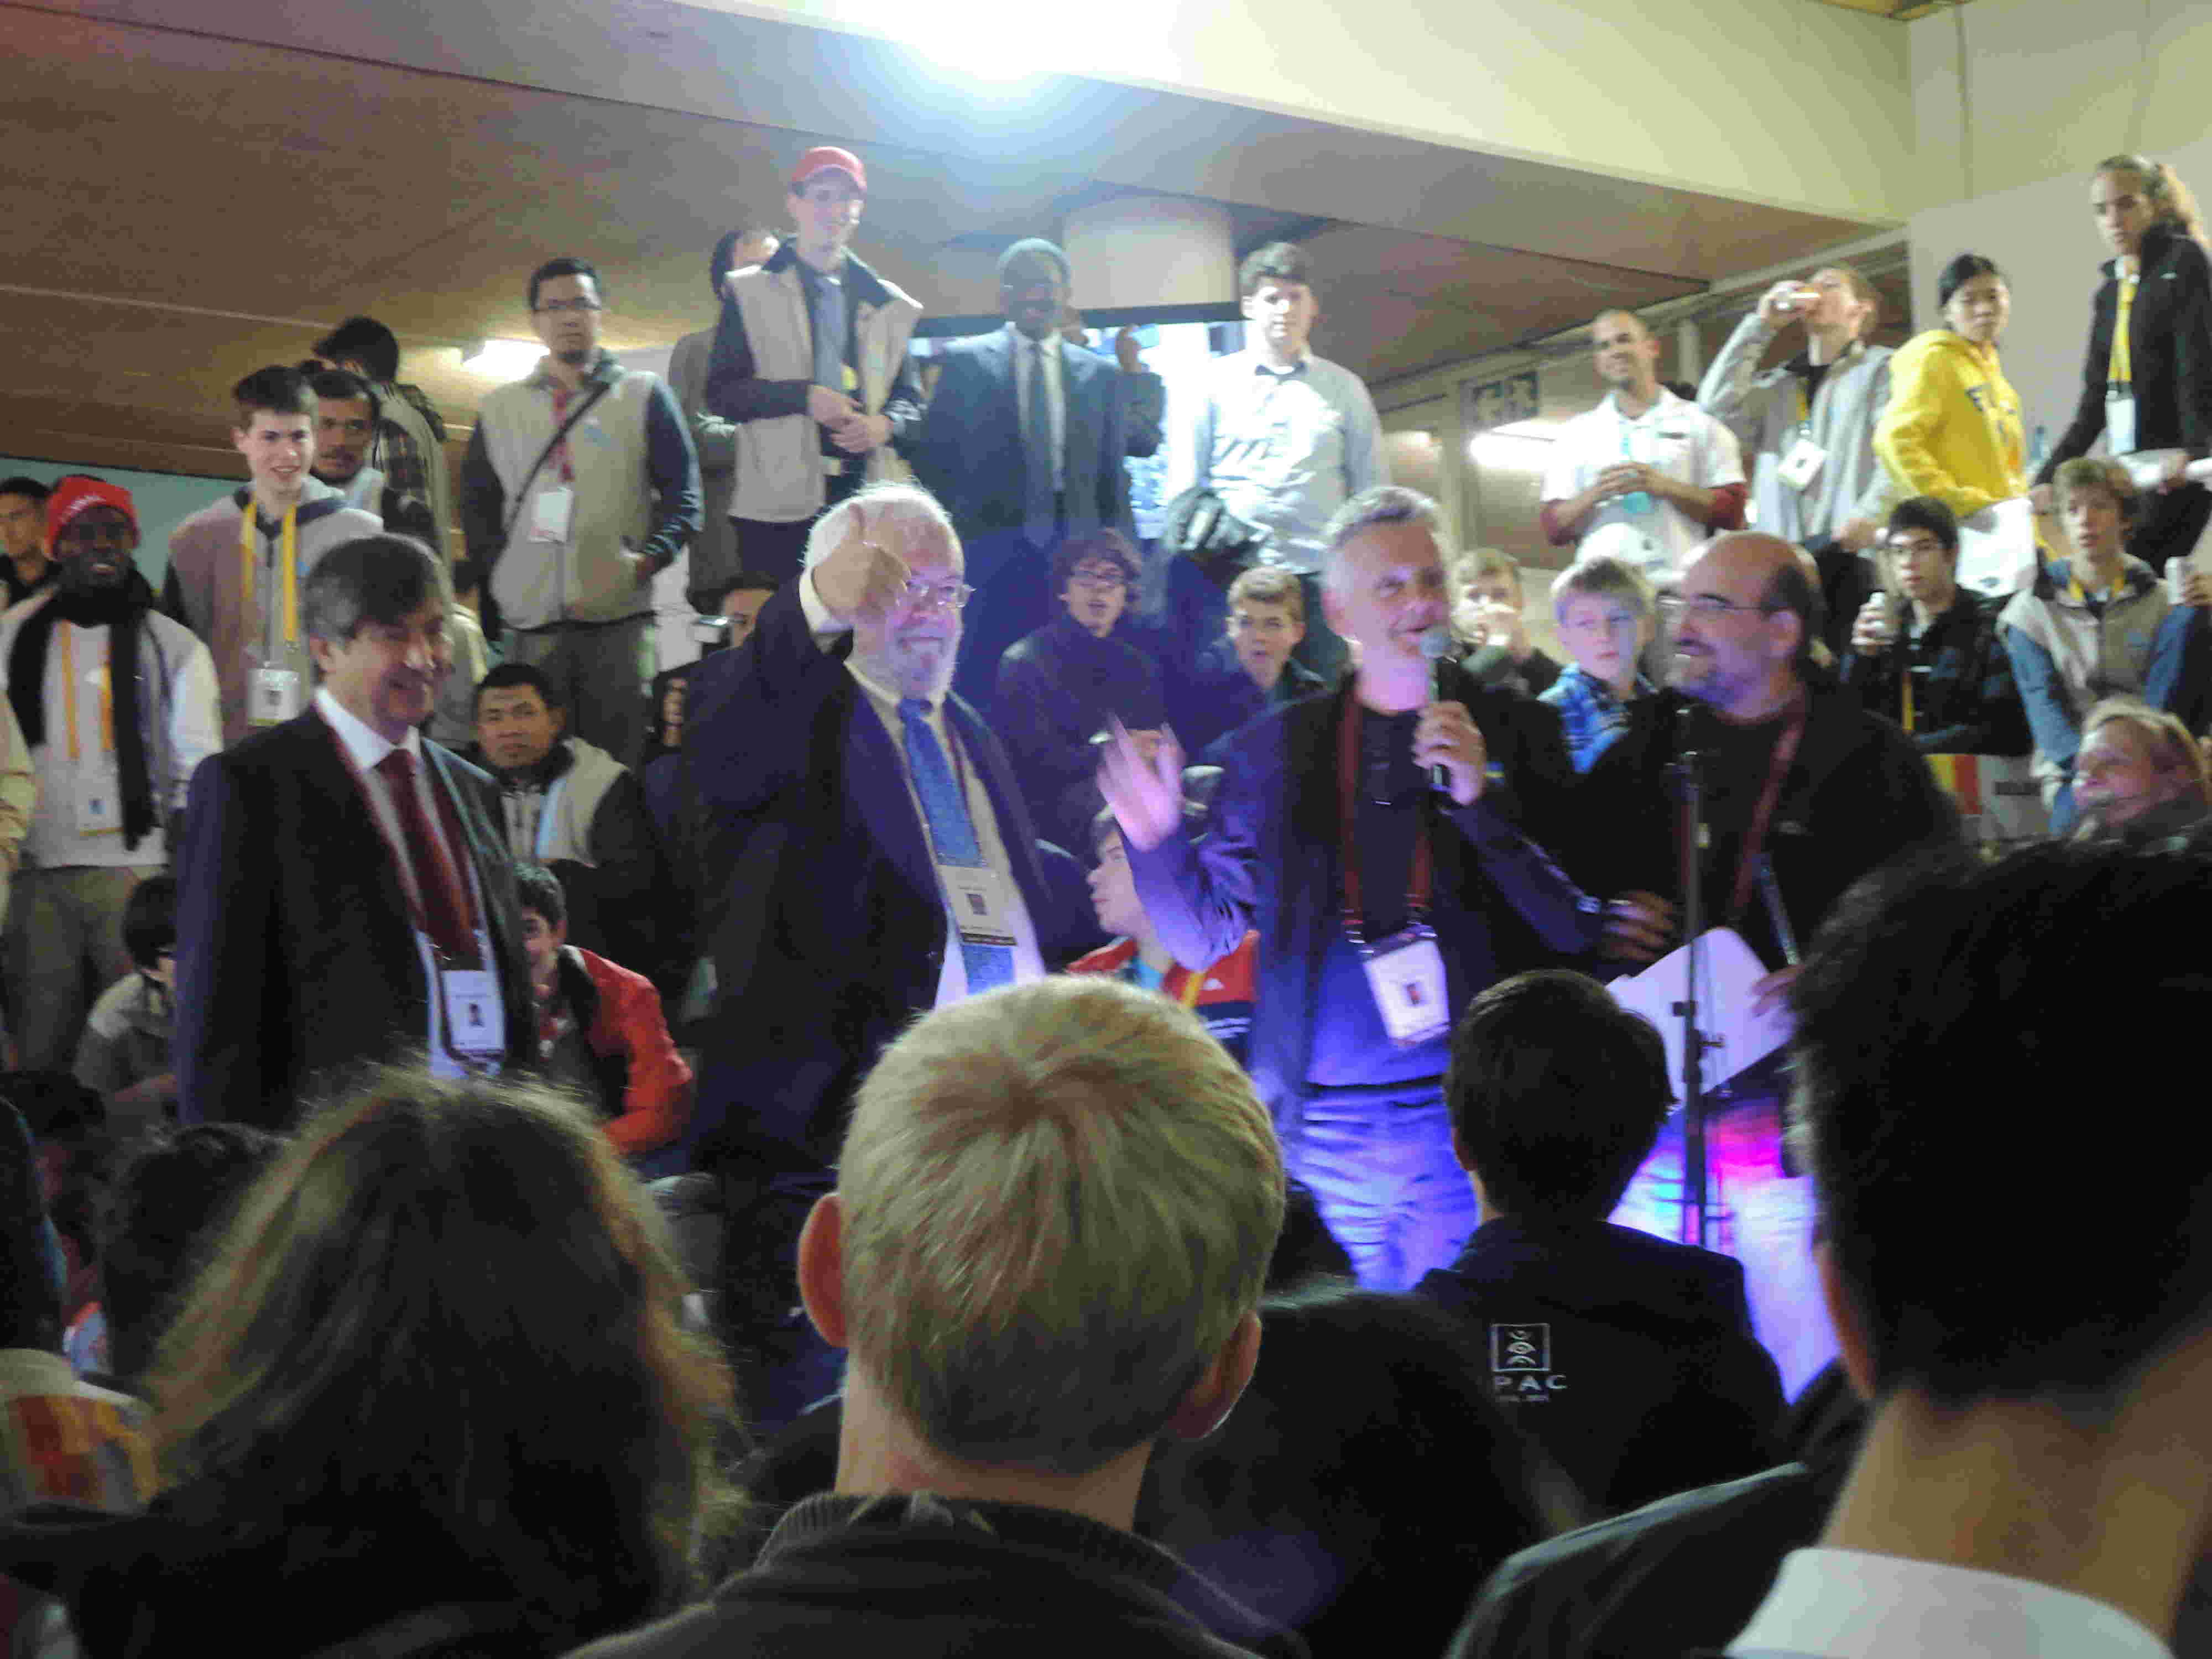
\includegraphics[width=0.5\textwidth]{media/geoff.jpg}
  \caption{Geoff wins the golden microphone.}
\end{figure}

A few biscuits, some photos, and a glass of non-alcoholic apple juice (I think) later, we head back
to pack for our departure from the 55th IMO tomorrow.

\section{July 13 -- Midnight Excursion}
I had heard from previous contestants about meeting lots of people from other teams.
I hadn't gotten to doing much of that, and I really regret it. So for anyone who
goes to compete at the IMO in the future, I recommend making a few friends and then asking
to crash rooms, as it seems most of the contestants cluster in single rooms on various floors.

The rest of the Taiwan team sleeps, but around 1AM I decide to not bother sleeping and discover one such
cluster on the sixth floor which is at the end of a Mafia game.
At some point we descend downwards to the games room where there are still
a few souls awake. We play some games of cards, and then play (or attempt to play) pool.
I would like to remark that pool is very hard.

In the last few hours of the morning I take a stroll through the UCT with one of the other graduating seniors.
We were originally looking for stars, but none are visible, and so we just walk and chat about our experiences
leading up to the IMO.
I would also like to confess to playing foosball and piano (Titanic again) near the leader's residence at 4AM.
I apologize if I woke anyone, though I don't think I did.
This was the happiest I had been in a long while.
We parted ways as the dawn broke, but needless to say we would meet again.

Thus I departed the University of Cape Town, marking the end of the night, the end of the 55th IMO,
and the end of the childhood dream I had chased for six years.

\end{document}
